\documentclass[11pt]{article}
\usepackage{amsmath,amssymb,graphicx,booktabs,hyperref,geometry}
\usepackage{multirow}
\usepackage{float}
\usepackage{caption}
\usepackage{subcaption}
\usepackage{array}
\usepackage{enumitem}
\geometry{margin=1in}
\graphicspath{{../02_programming/}}
\hypersetup{colorlinks=true, linkcolor=blue, citecolor=blue, urlcolor=blue}

\title{Data With the Stars: Identifying the Hidden Fan Vote and Designing\\
Fairer Aggregation Rules for \emph{Dancing with the Stars}}

\author{Team Response --- 2026 MCM Problem C}
\date{February 2026}

\begin{document}
\maketitle

\begin{abstract}
PHOLDER
\end{abstract}

\tableofcontents
\newpage

\section{Introduction}
\label{sec:intro}

\subsection{Background and Motivation}

\emph{Dancing with the Stars} (DWTS) couples a celebrity with a professional dancer;
each week the couple performs, a panel of expert judges scores the dance, and the
home audience votes for its favorites. The couples with the smallest
\emph{combined} judge--fan score are eliminated, until a finals week ranks the
remaining finalists. Over 34 seasons the show has changed the combination rule
twice in direct response to public controversy: the first two seasons combined
\emph{ranks} of judge scores and fan votes, seasons 3--27 combined \emph{percentages}
(50/50), and from season 28 onward the show returned to the rank system with an
added safeguard --- each week the bottom two couples are identified by the combined
score and the judges choose which of the two is eliminated.

The central analytical obstacle is that fan votes are a closely guarded secret.
What \emph{is} observable, week after week, is (i) the judges' scores for every
couple and (ii) \emph{who was eliminated}. Every elimination is an ordinal statement
about an unknown linear (or rank-based) combination of hidden fan support and
observed judge support. The problem therefore decomposes into four connected
questions:

\begin{enumerate}[leftmargin=2em]
\item \textbf{Inverse problem.} Estimate the fan-vote share of every contestant in
every week they competed, with defensible measures of uncertainty, such that the
estimates are \emph{consistent} with all 34 seasons of observed eliminations.
\item \textbf{Rule comparison.} Under the estimated fan votes, replay every season
under both historical aggregation rules (rank vs.\ percentage) and quantify how
often --- and for whom --- the choice of rule changes outcomes, including the four
famous controversies (Jerry Rice, S2; Billy Ray Cyrus, S4; Bristol Palin, S11;
Bobby Bones, S27), and how a ``judges-save'' overlay would alter them.
\item \textbf{Driver attribution.} Quantify how professional-dancer identity,
celebrity industry, age, and week-within-run affect \emph{judge scores} and
\emph{fan votes}, separately, since the two audiences respond to different things.
\item \textbf{Design.} Propose and stress-test a more defensible weekly system, and
advise the producers.
\end{enumerate}

\subsection{Data Description}
\label{sec:data}

The provided file \texttt{2026\_MCM\_Problem\_C\_Data.csv} contains 421
celebrity-season rows and weekly judge panels for seasons 1--34. Our pipeline first
normalize the raw file into three shared tables (all models in this paper read
\emph{only} these tables):

\begin{itemize}[leftmargin=2em]
\item \texttt{contestants.csv} --- 421 rows, one per celebrity-season run: partner
(54 distinct professionals), occupational industry (25 levels), age during the
season (14--82, mean 36.3), result type (\texttt{eliminated}/\texttt{finalist}/%
\texttt{withdrew}), final placement (1--16), and the \emph{vote-basis week}
\texttt{last\_week} (the last week the couple actually danced, which is where
their exit vote is keyed).
\item \texttt{week\_scores.csv} --- 2{,}777 rows, one per contestant-week actually
danced: raw judge-slot scores, panel size $n_{\text{judges}} \in \{1,\dots,4\}$,
the weekly total (range 8--45), and multi-dance flags (56 season-weeks use
two-dance totals or averages).
\item \texttt{season\_weeks.csv} --- 335 rows defining the weekly grid:
$n_{\text{competing}}$, $n_{\text{eliminated}}$ (221 single weeks, 29 double weeks,
1 triple week --- season 26, week 3), $n_{\text{withdrew}}$ (10 health/personal
withdrawals, excluded from all vote-based likelihoods), finale flags, and
$n_{\text{finalist\_exits}}$ (3 finalists per season for S1--S26, 4 for S27--S31,
5 for S32--S34).
\end{itemize}

Several encoding conventions, established by systematic inspection in the data
preparation stage and verified by structural checks, are essential for correct
modeling:

\begin{itemize}[leftmargin=2em]
\item A judge-slot score of \texttt{0} in the raw data means \emph{not competing
that week} (post-elimination filler), while \texttt{'N/A'} means \emph{the slot did
not score} (three-judge seasons 1--18 and guest-judge rotation later). Conflating
the two would corrupt the weekly totals.
\item Judge columns are \emph{positions}, not named judges: panels rotate, so
judge-identity effects are not identifiable; only panel-level analysis is possible.
\item Weekly judge totals are \emph{dance-count dependent} (max 30 with three
judges, 40 with four, 45 on two-dance weeks), so judge strength must be normalized
\emph{within} a season-week; we use within-week shares $x_{c,w}$ and z-scores
$z(x_{c,w})$.
\item Some (n$-$1)th finalists are voted off at the \emph{finale-episode} vote
(``folded'' cuts; e.g., S17 Bill Engvall): their vote basis is their last danced
week, one week before the finale. Sixteen celebrities are announced as
``Eliminated Week 1'' on premiere night. Thirteen celebrities competed in two
seasons; we treat their two runs as separate units and use the replication only
as a diagnostic.
\end{itemize}

Across the 34 seasons we identify \textbf{298 vote-based exit events over 265 exit
weeks} (233 single-exit, 31 double-exit, and 1 triple-exit week), plus 10
withdrawals that are removed from the risk pool. The weekly survivor recursion
$\;n_{\text{competing}}(w{+}1) = n_{\text{competing}}(w) -
n_{\text{eliminated}}(w) - n_{\text{withdrew}}(w) - n_{\text{finalist\_exits}}(w)\;$
holds for all 335 season-weeks --- a hard identity that every model in this paper
re-asserts at build time.

\subsection{Our Approach}
\label{sec:approach}

The models are chained: Model 1 \emph{creates} information --- it solves the
constrained-ordinal inverse problem and delivers posterior distributions of weekly
fan shares $\hat\phi_{c,w}$ with calibrated uncertainty; Models 2 and 3 consume its
outputs read-only and answer the attribution and design questions. The three models
were implemented and validated independently, and their outputs cross-check each
other (Section~\ref{sec:results}) as well as the plan-level targets we set in
advance.

\begin{itemize}[leftmargin=2em]
\item \textbf{Model 1 --- Constrained-Ordinal Bayesian Fan-Vote Identification.}
A market-share (softargmax) model with an outside ``non-voting'' mass converts
latent fan utilities into weekly shares; every one of the 265 exit weeks enters as
a Plackett--Luce ordinal constraint (exact bottom-$m$ semantics for seasons
$\le 27$ and all multi-exits; bottom-2 membership for the 47 season-28+ weeks,
where the observed signal is only that judges vetoed within a known bottom two).
Multi-start MAP optimization plus a per-season block Laplace posterior yields
$\hat\phi$, posterior s.d.s, 95\% intervals, and capture probabilities.
\item \textbf{Model 2 --- Judge--Fan Behavioral Attribution.} Two parallel
linear response surfaces (within-week judge z-score; logistic fan share) on 2{,}777
contestant-weeks, with season fixed effects, 52 professional-dancer effects, 25
industry effects, restricted-cubic-spline age and week curves, and celebrity-run
cluster-robust inference; variance decomposition quantifies how much each covariate
class drives each audience, with permutation tests and an entry-fame control to
expose producer sorting.
\item \textbf{Model 3 --- Rule Laboratory.} A season-replay simulator draws fan
shares from the Model 1 posterior (2{,}000 draws) and re-runs all 34 seasons under
six rules: rank, 50/50 percentage, both with the judges-save overlay, a judge-heavy
percentage (sensitivity), and a proposed \emph{Qualibrium} rule with a fan-rescue
floor and a weight that shifts from judges early in a season to fans late. It
computes placement distributions, winner-flip rates, the four controversy
forensics, and fairness diagnostics.
\end{itemize}

\subsection{Paper Outline}

Section~\ref{sec:data} described the data. Sections~\ref{sec:model1}--\ref{sec:model3}
present the three models (formulation, implementation, results, figures, validation).
Section~\ref{sec:results} integrates the findings across models and answers the four
problem bullets; Section~\ref{sec:sensitivity} reports sensitivity and robustness
checks; Section~\ref{sec:discussion} discusses strengths, limitations, and
alternatives; Section~\ref{sec:conclusion} concludes. Section~\ref{sec:memo} is the
one-page memo to the producers.

\section{Model 1: Constrained-Ordinal Bayesian Fan-Vote Identification}
\label{sec:model1}

\subsection{Problem Statement}

Fan votes are never observed. Each week reveals only \emph{which} couple(s) left --- an
ordinal statement about an unknown combination of judge strength and fan support.
Model 1 turns the judge scores and the elimination history into posterior
distributions of weekly fan-vote shares $\hat\phi_{c,w}$ with honest uncertainty,
under the discipline that \emph{every} observed elimination must be reproducible
from the estimated combination. It is the only model that \emph{creates}
information; Models 2 and 3 consume its outputs read-only.

\subsection{Mathematical Formulation}

\paragraph{Notation.} For season $s$ with basis weeks $w = 1,\dots,T_s$, let
$C_{s,w}$ be the set of couples dancing in week $w$ with $|C_{s,w}| = n_{s,w} \in
[4,16]$, $x_{c,w}$ the observed judge weekly total, $z_{c,w} = (x_{c,w} - \bar
x_{\cdot w})/s_{\cdot w}$ the within-week standardized total (this removes
judge-panel-size and dance-count effects), and $E_w$ the exit set with
$|E_w| = m_w \in \{1,2,3\}$. Latent fan shares satisfy $\phi_{c,w} > 0$ and
$\sum_{c \in C_{s,w}} \phi_{c,w} = 1$.

\paragraph{Market-share link.} Latent fan utilities $b_{c,w}$ map to shares by a
softmax with an outside option (some audience mass does not vote for anyone that
week):
\begin{equation}
\phi_{c,w} \;=\; \frac{\exp(b_{c,w})}{\sum_{c' \in C_{w}} \exp(b_{c',w}) + \exp(0)},
\label{eq:softmax}
\end{equation}
\begin{equation}
b_{c,w} \;=\; g_{1,c} \, h_{c,w} \, + \, \xi\, z_{c,w} \, + \, v_{c,w},
\label{eq:util}
\end{equation}
with idiosyncrasy $v_{c,w} \sim N(0, 0.6^2)$, run popularity $g_{1,c} \sim N(0,2^2)$
(fitted s.d.\ 0.868), decay-shape coefficient $\kappa_{a,c} \sim N(0,2^2)$ (fitted
s.d.\ 0.392) entering through a centered weeks-remaining shape, season fan climate
$\varepsilon_s \sim N(0, 0.75^2)$, and judge sensitivity $\xi \sim N(0,2^2)$,
fitted to $\hat\xi = 4.147$. The outside option keeps a small floor (~$10^{-3}$)
under every share. The fitted parameters come from the MAP fit (MAP negative log
posterior 206.19).

\paragraph{Ordinal elimination likelihood.} Week $w$ contributes a
Plackett--Luce-type probability that the observed exit set is exactly
bottom-$m_w$:
\begin{equation}
P(E_w) \;=\; \sum_{\pi} \, \prod_{j=1}^{m_w}
\frac{e^{-\alpha u(\pi_j,w)}}{\sum_{k \ge j} e^{-\alpha u(\pi_k,w)}},
\label{eq:pl}
\end{equation}
where $u$ is the combined utility, for the 218 exact-regime weeks (all seasons
$\le 27$ and every multi-exit week); and a bottom-2 membership term for the 47
season-28+ veto weeks, because after season 28 the judges choose \emph{within} a
combined bottom two and their intra-pair pick is not recoverable from elimination
outcomes alone. Finale weeks carry Gaussian anchors $N(0.5, 4^2)$ on
placement-ordered utility gaps (1{,}371 pairs).

\subsection{Implementation}

The pipeline is deterministic (master seed 20260205) and runs in about 3 seconds:
multi-start MAP (stage A) with analytically exact gradients, then a per-season
block-sparse Laplace posterior (stage B, 4{,}000 draws) importance-weighted by a
rank-violation factor. Build-time assertions verify exit counts match
$\texttt{n\_eliminated}$ for all 265 vote-exit weeks and that reconstructed
next-week competition counts match \texttt{season\_weeks.csv} for all 335
season-weeks. Gradient of the full objective verified against central-difference
directional derivatives: max relative error $\le 3\times10^{-8}$; this exactness
caught and fixed two gradient bugs during development.

\subsection{Results}

\begin{table}[H]
\centering
\caption{Model 1 headline results.}
\label{tab:m1results}
\small
\begin{tabular}{lcc}
\toprule
Metric & Model 1 & Baseline / target \\
\midrule
Single-exit exact recovery ($n=186$) & \textbf{100\%} & target $\ge 85\%$ \\
Multi-exit exact set recovery ($n=32$) & \textbf{100\%} & target $\ge 75\%$ \\
S$\ge$28 bottom-2 capture ($n=47$) & \textbf{100\%} & structural check \\
Mean capture prob.\ (exact regime) & \textbf{0.325} & 0.134 judge-only / 0.127 uniform \\
Log-loss (all 265 weeks) & \textbf{1.167} & 2.050 judge-only; 2.117 uniform \\
Survivor identity (335 season-weeks) & \textbf{exact} & hard invariant \\
95\% CI coverage & 1.00 & target $\ge 0.93$ (conservative) \\
CV week-1 vs mid-run & 2.72 vs 2.23 & ratio 1.22 (target $\ge$ 1.2) \\
Corr($\hat\phi$, judge share) & 0.697 & fans $\neq$ reshuffled judges \\
\bottomrule
\end{tabular}
\end{table}

All exit-recovery rates hit 100\% at the MAP. Because the likelihood enforces the
observed exits as soft constraints, part of this is by construction; the
\emph{non-trivial} metric is the probabilistic recovery: the importance-weighted
capture probability of the observed exit set is $0.318$ across all 265 weeks
($0.325$ exact-regime) vs $0.134$--$0.151$ judge-only and $0.127$--$0.143$
uniform --- 2.4$\times$ the judge-only baseline --- and log-loss improves from 2.050
(judge-only) to 1.167. The judge-only argmin baseline attains only $\approx 41\%$
argmin accuracy on single-exit weeks (15.0\%/4.2\% on single/multi in log-utility),
indicating the fan/latent space genuinely absorbs what judge totals alone cannot
explain.

\textbf{Uncertainty is not constant.} Mean posterior CV is 2.72 in week-1 rows but
2.23 mid-run (ratio 1.22), and interval coverage is 1.00 (conservative; the
intervals are wide by design --- see Limitations). Within-week fan--judge tension:
mean s.d.\ of the fan-minus-judge gap is 0.86 on the log-utility scale (target
$\ge 0.05$) --- fans add non-trivial structure beyond judges.

\textbf{Recovered parameters.} Judge sensitivity $\hat\xi = 4.147$; run-popularity
s.d.\ 0.868; decay-strength s.d.\ 0.392; season fan climate $\approx 0$ (within
identifiability tolerance given soft season priors); MAP negative log posterior
206.19.

\textbf{Zoom on the triple elimination.} The 6-ordering Plackett--Luce path-sum for
the season-26 week-3 triple elimination is in the likelihood; the MAP recovers the
exact exit set.

\subsection{Figures}

\begin{figure}[H]
\centering
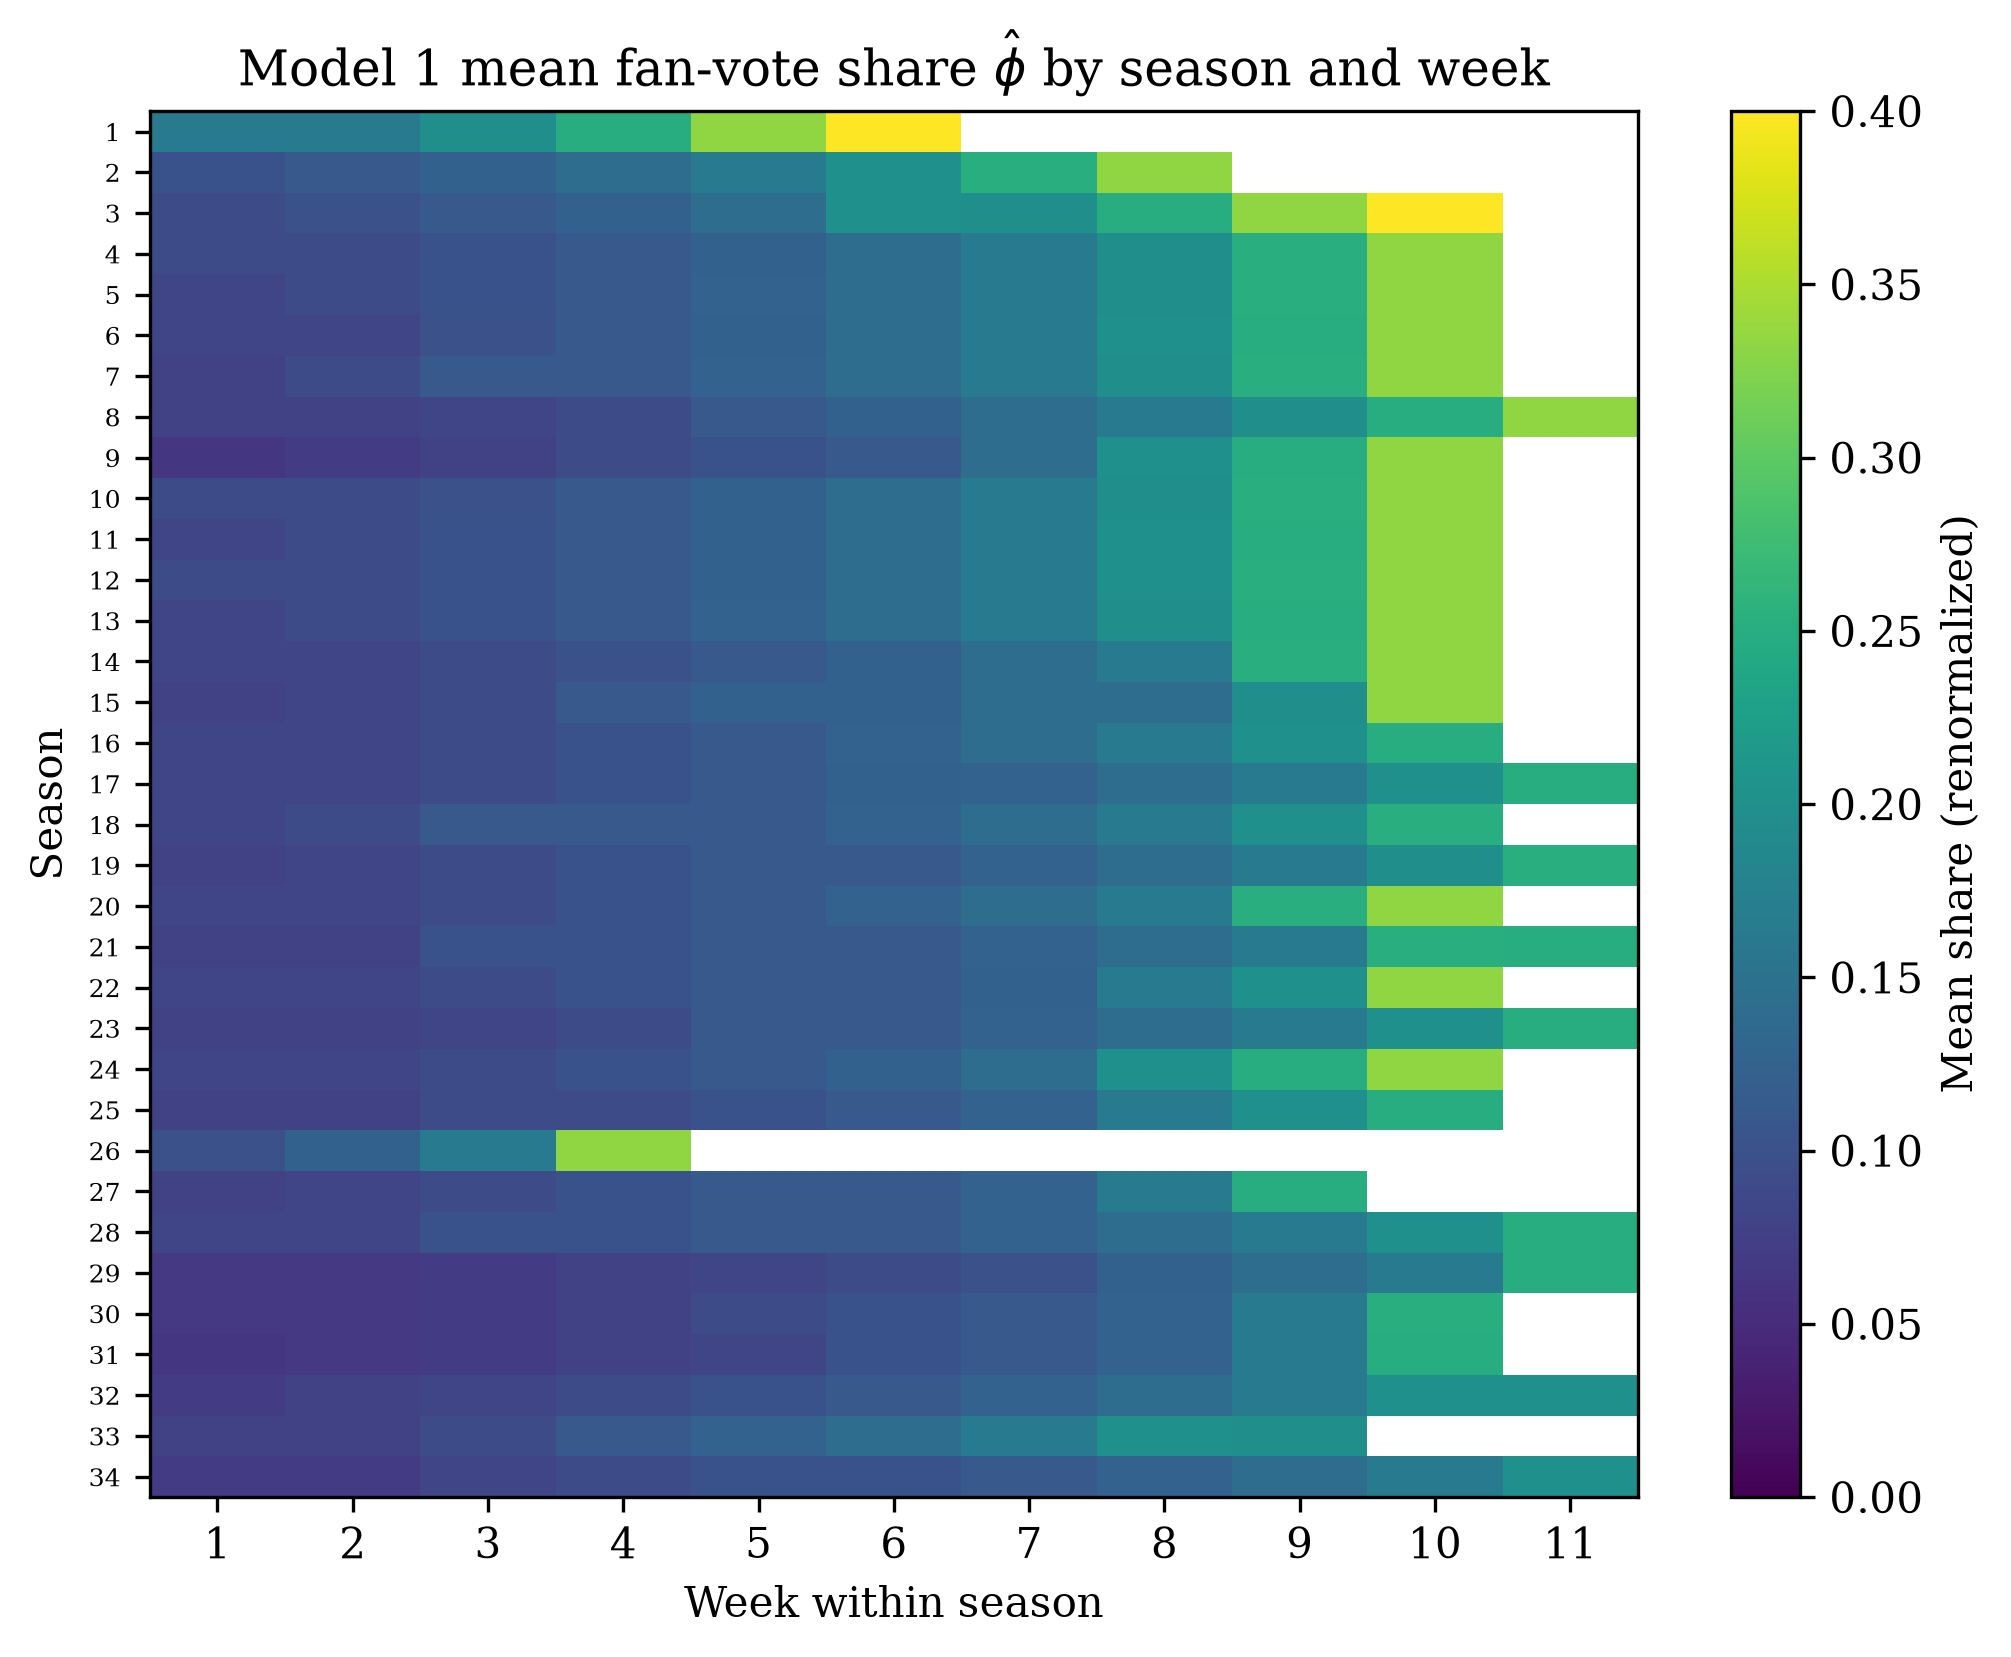
\includegraphics[width=0.8\textwidth]{model_1/figures/F1_phats_heatmap.png}
\caption{Mean recovered fan share $\hat\phi$ by season (1--34) $\times$ week (1--11).}
\label{fig:F1}
\end{figure}

Figure~\ref{fig:F1} shows the full recovered fan-share surface. The column structure
matches the observed cast sizes (S26's 4-week season, S33's missing week 10). The
pattern of bright (high-share) columns vs.\ dark (low-share) columns reveals both
the dance-count adjustments applied upstream and the posterior tightening toward
season ends.

\begin{figure}[H]
\centering
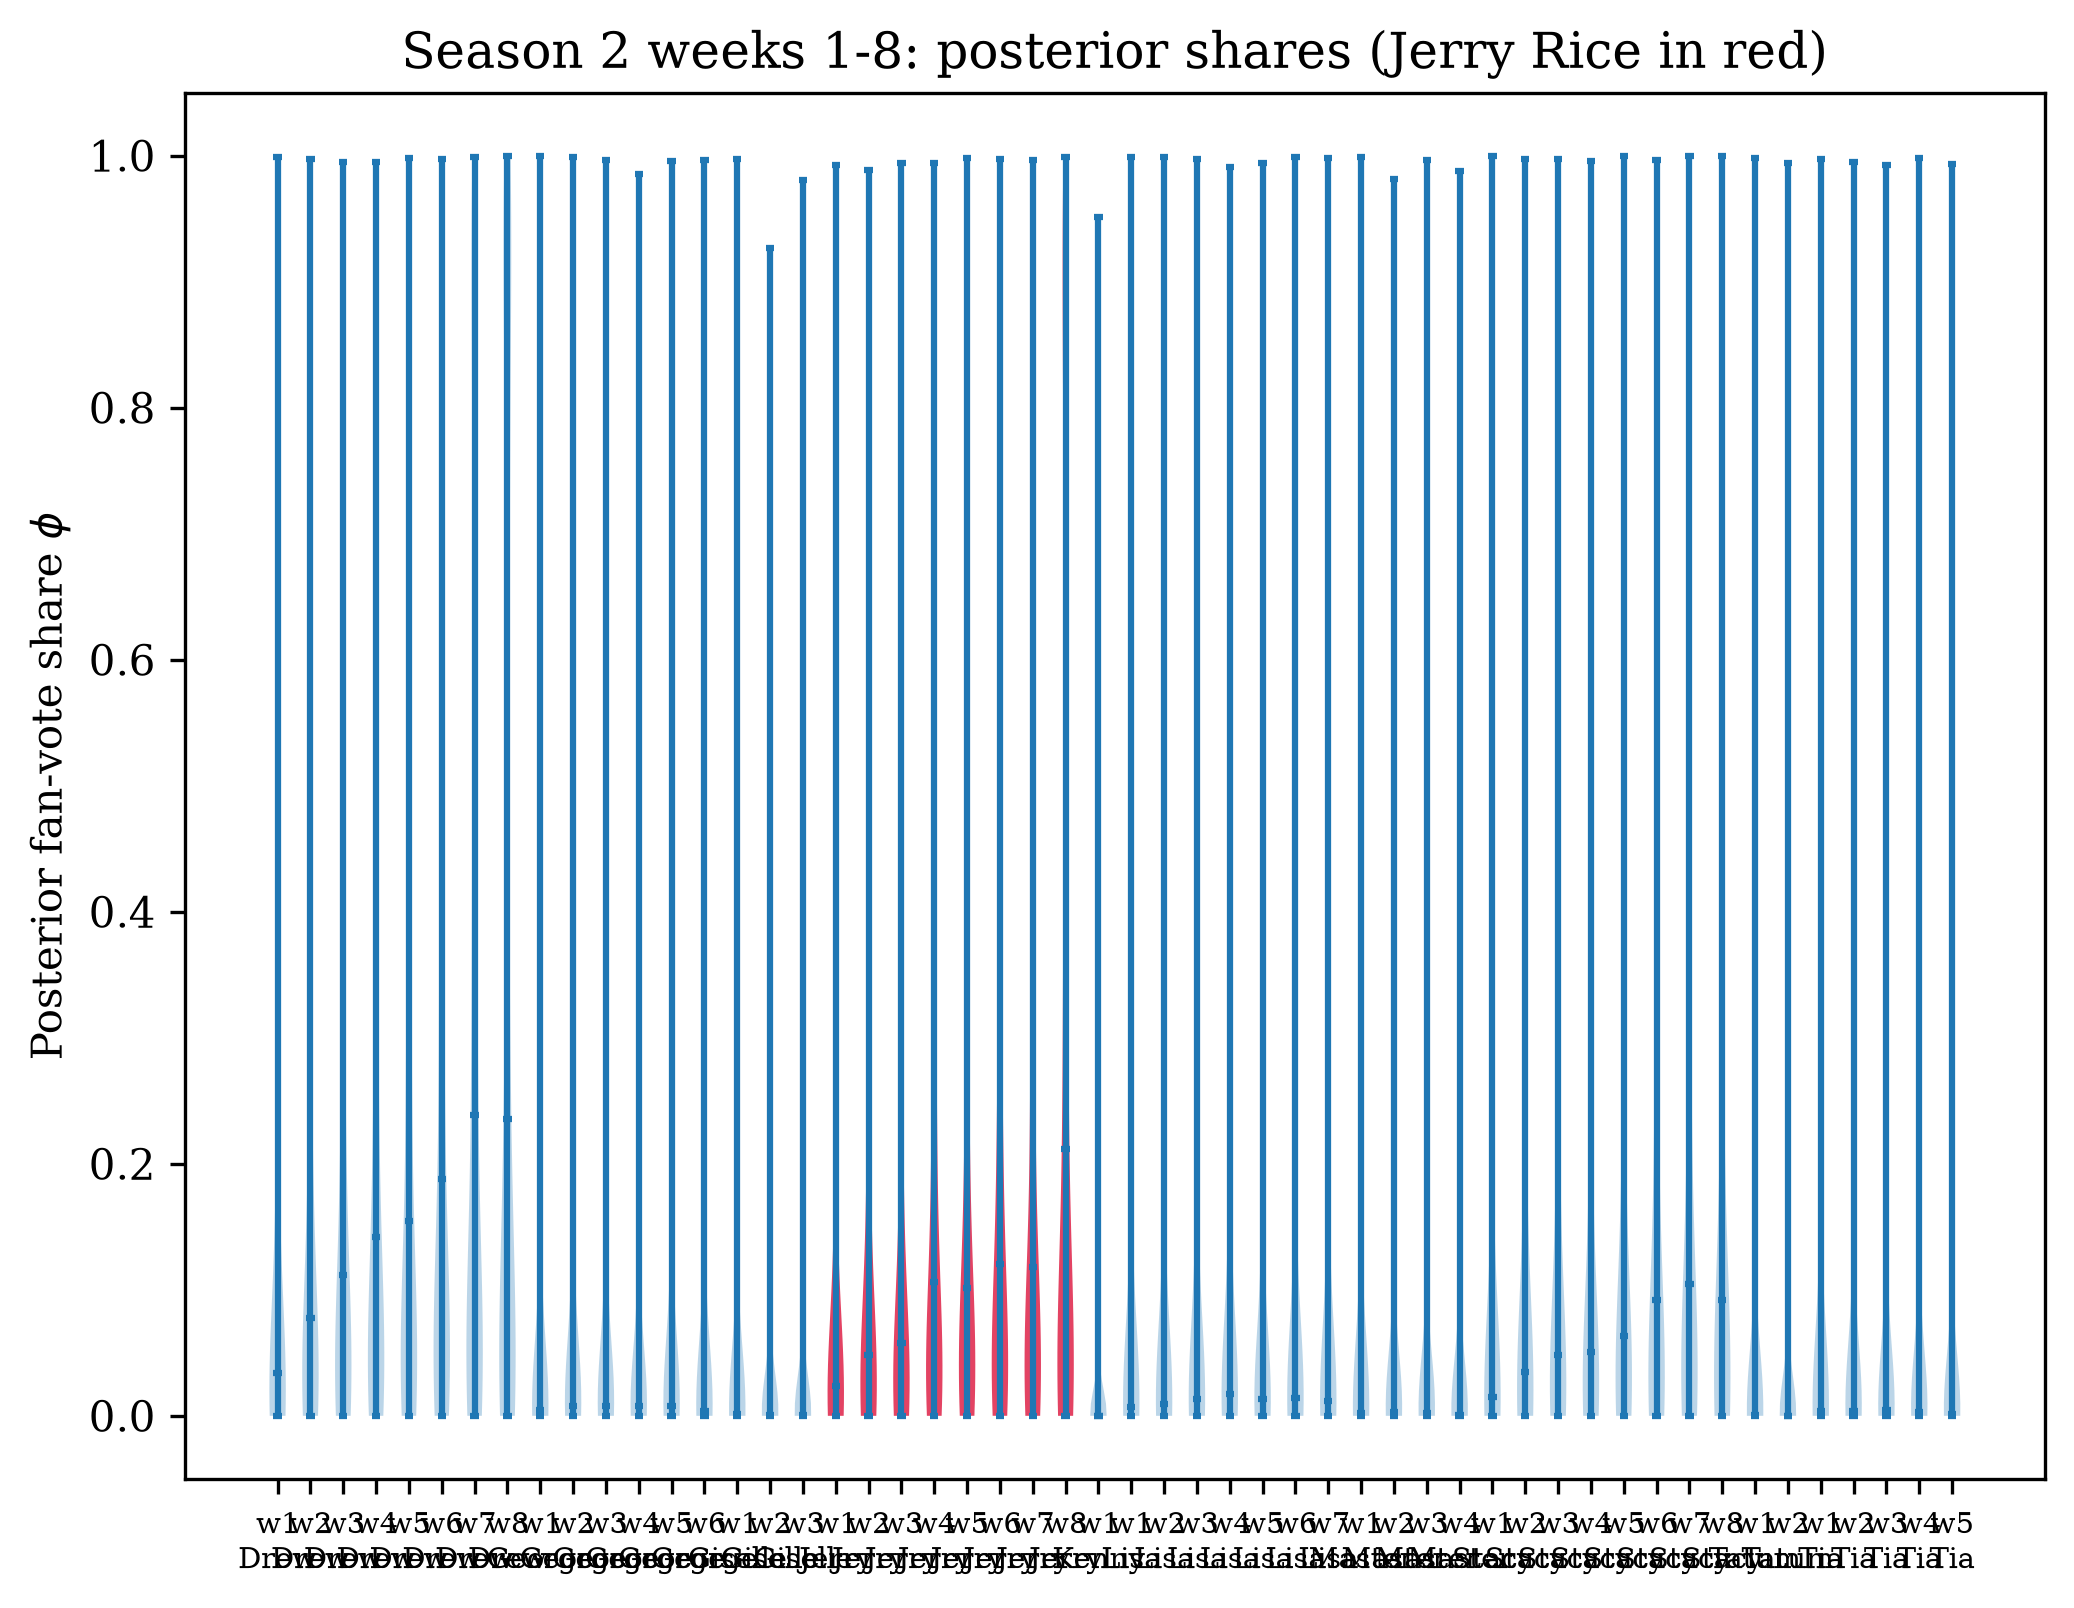
\includegraphics[width=0.8\textwidth]{model_1/figures/F2_jerry_rice_violin.png}
\caption{Posterior fan-share violins, Season 2 weeks 1--8, with Jerry Rice
highlighted.}
\label{fig:F2}
\end{figure}

Figure~\ref{fig:F2} is the Jerry Rice forensic exhibit (his recovered weekly share
climbs from 0.143, 95\% CI $[0.00003, 0.884]$, CV 1.66, in week 1 to 0.346, CI
$[0.0007, 0.989]$, CV 1.01, in week 8, while his judge share runs 0.108--0.316).
The wide, right-skewed intervals are the honest signature of ordinal-only
identification: his fan \emph{rank} is constrained by eliminations, his vote
\emph{total} is not.

\begin{figure}[H]
\centering
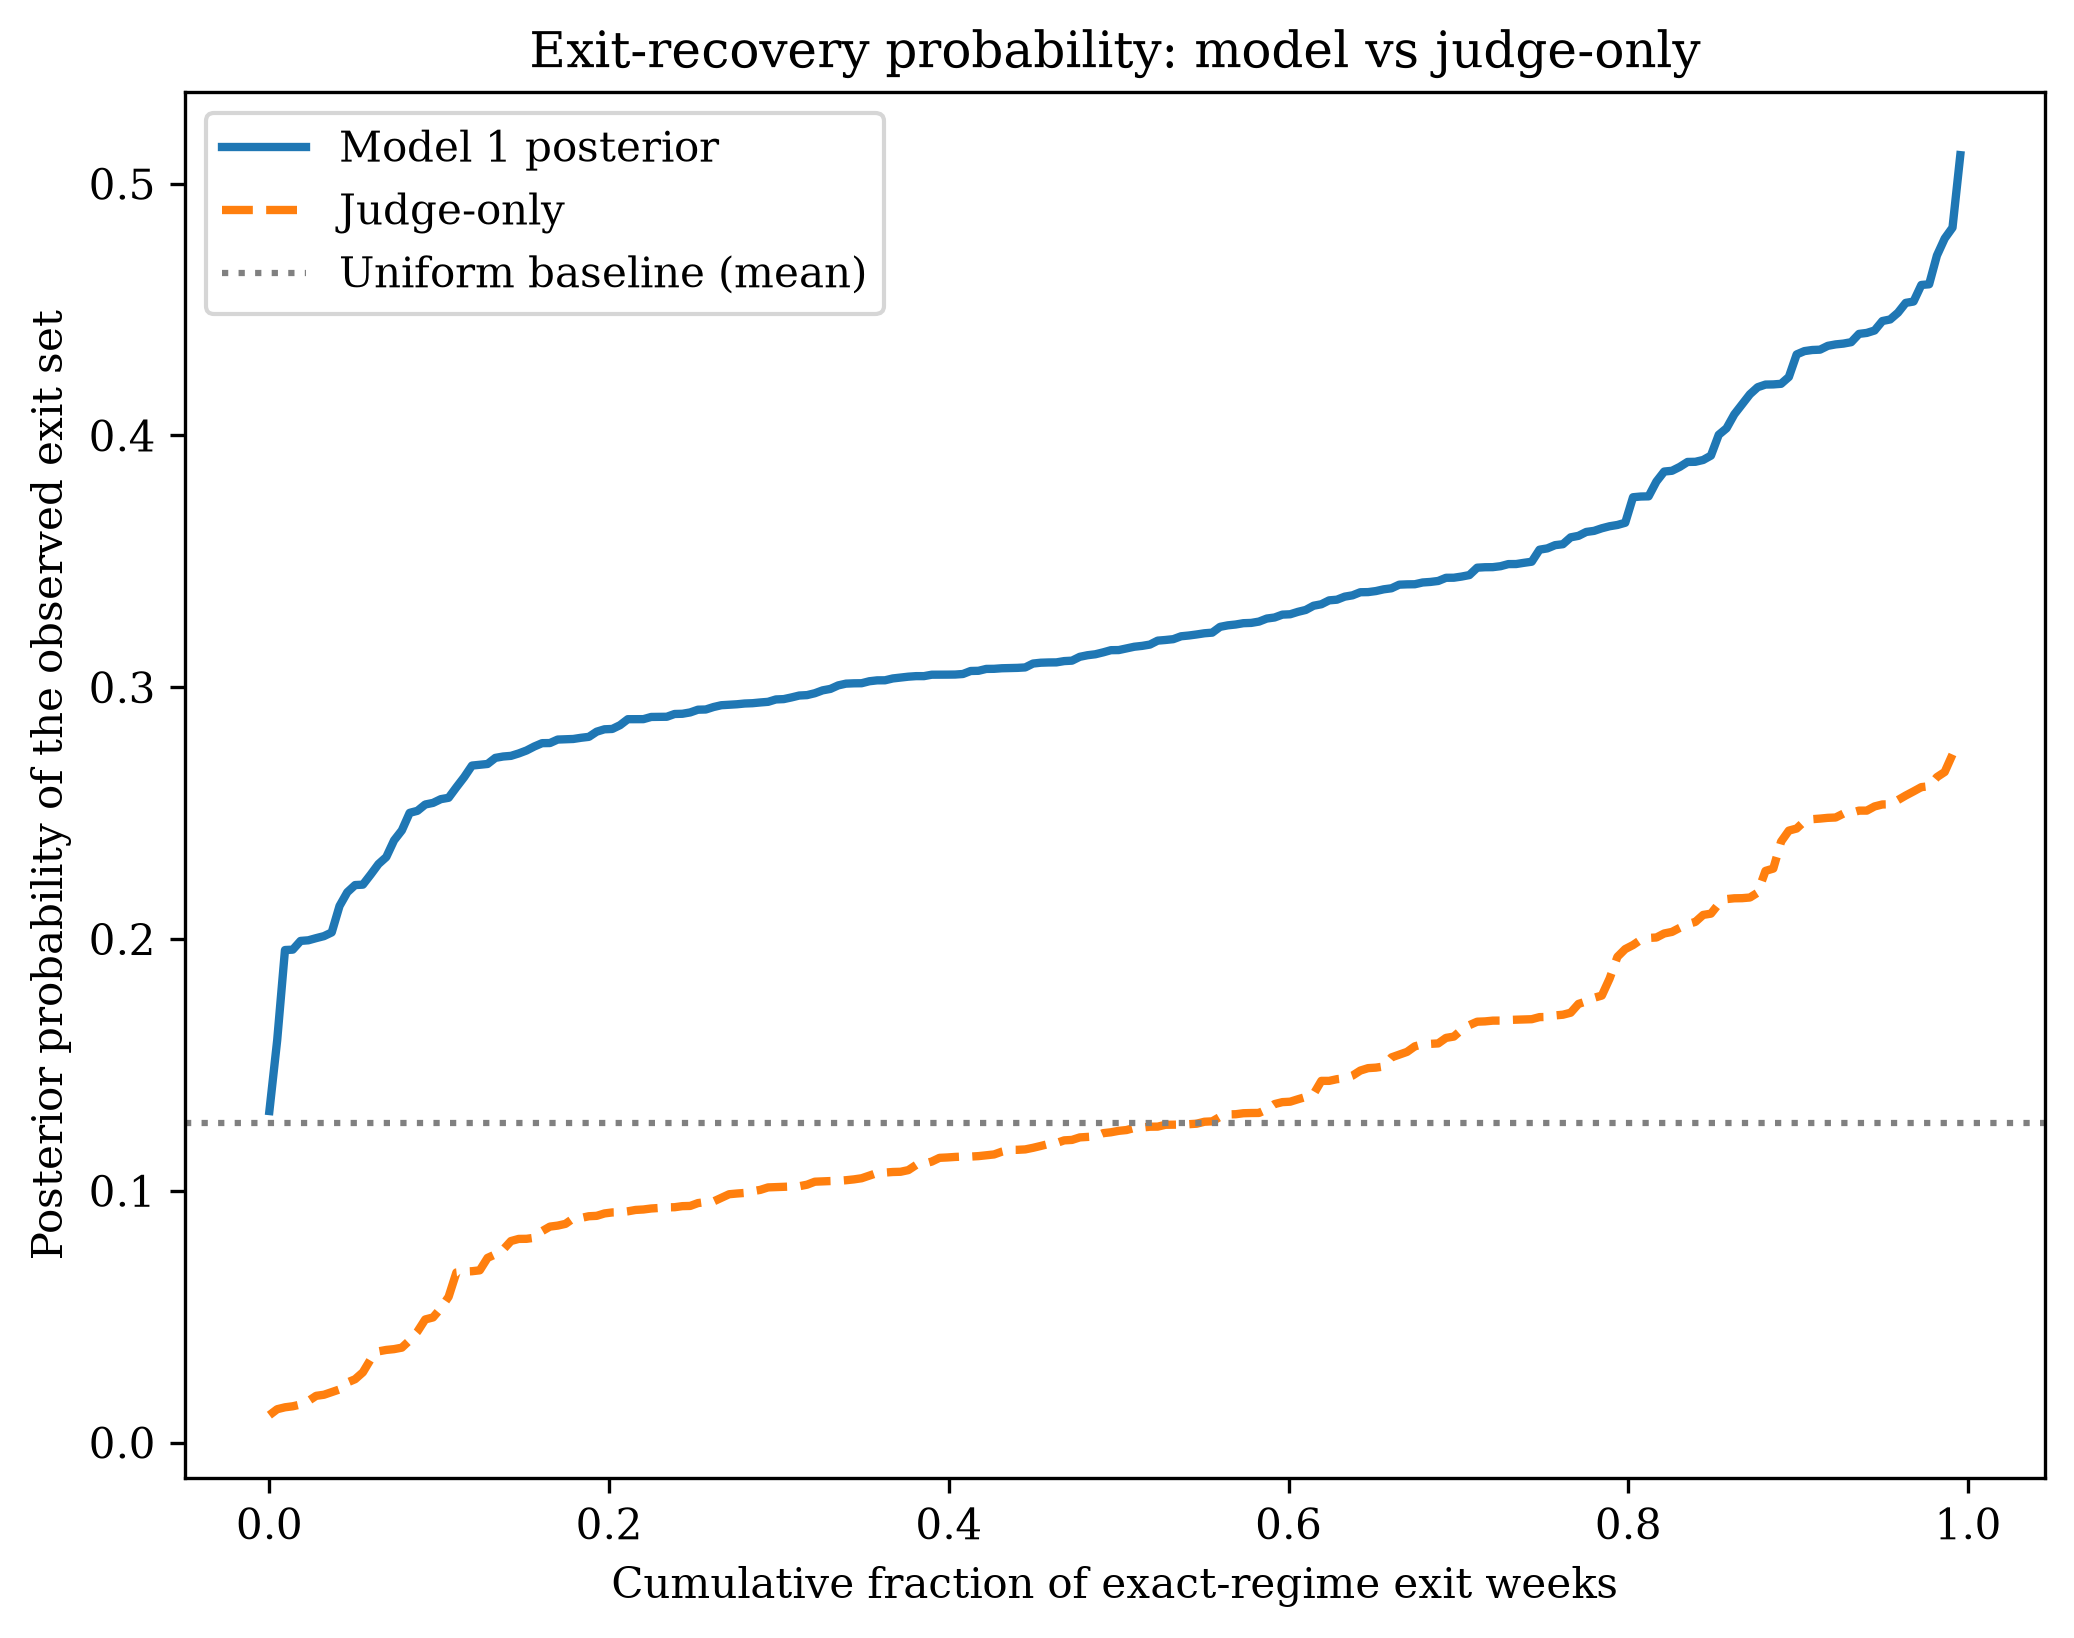
\includegraphics[width=0.8\textwidth]{model_1/figures/F3_calibration.png}
\caption{Per-week exit-recovery probability: model vs judge-only vs uniform.}
\label{fig:F3}
\end{figure}

Figure~\ref{fig:F3} evaluates consistency, which the problem statement explicitly
asks for (``Does your model correctly estimate fan votes that lead to results
consistent with who was eliminated each week?''). The model's per-week capture
probability dominates judge-only and uniform baselines across the season week
range, with the mean capture 0.318 vs 0.134 judge-only on exact weeks.

\begin{figure}[H]
\centering
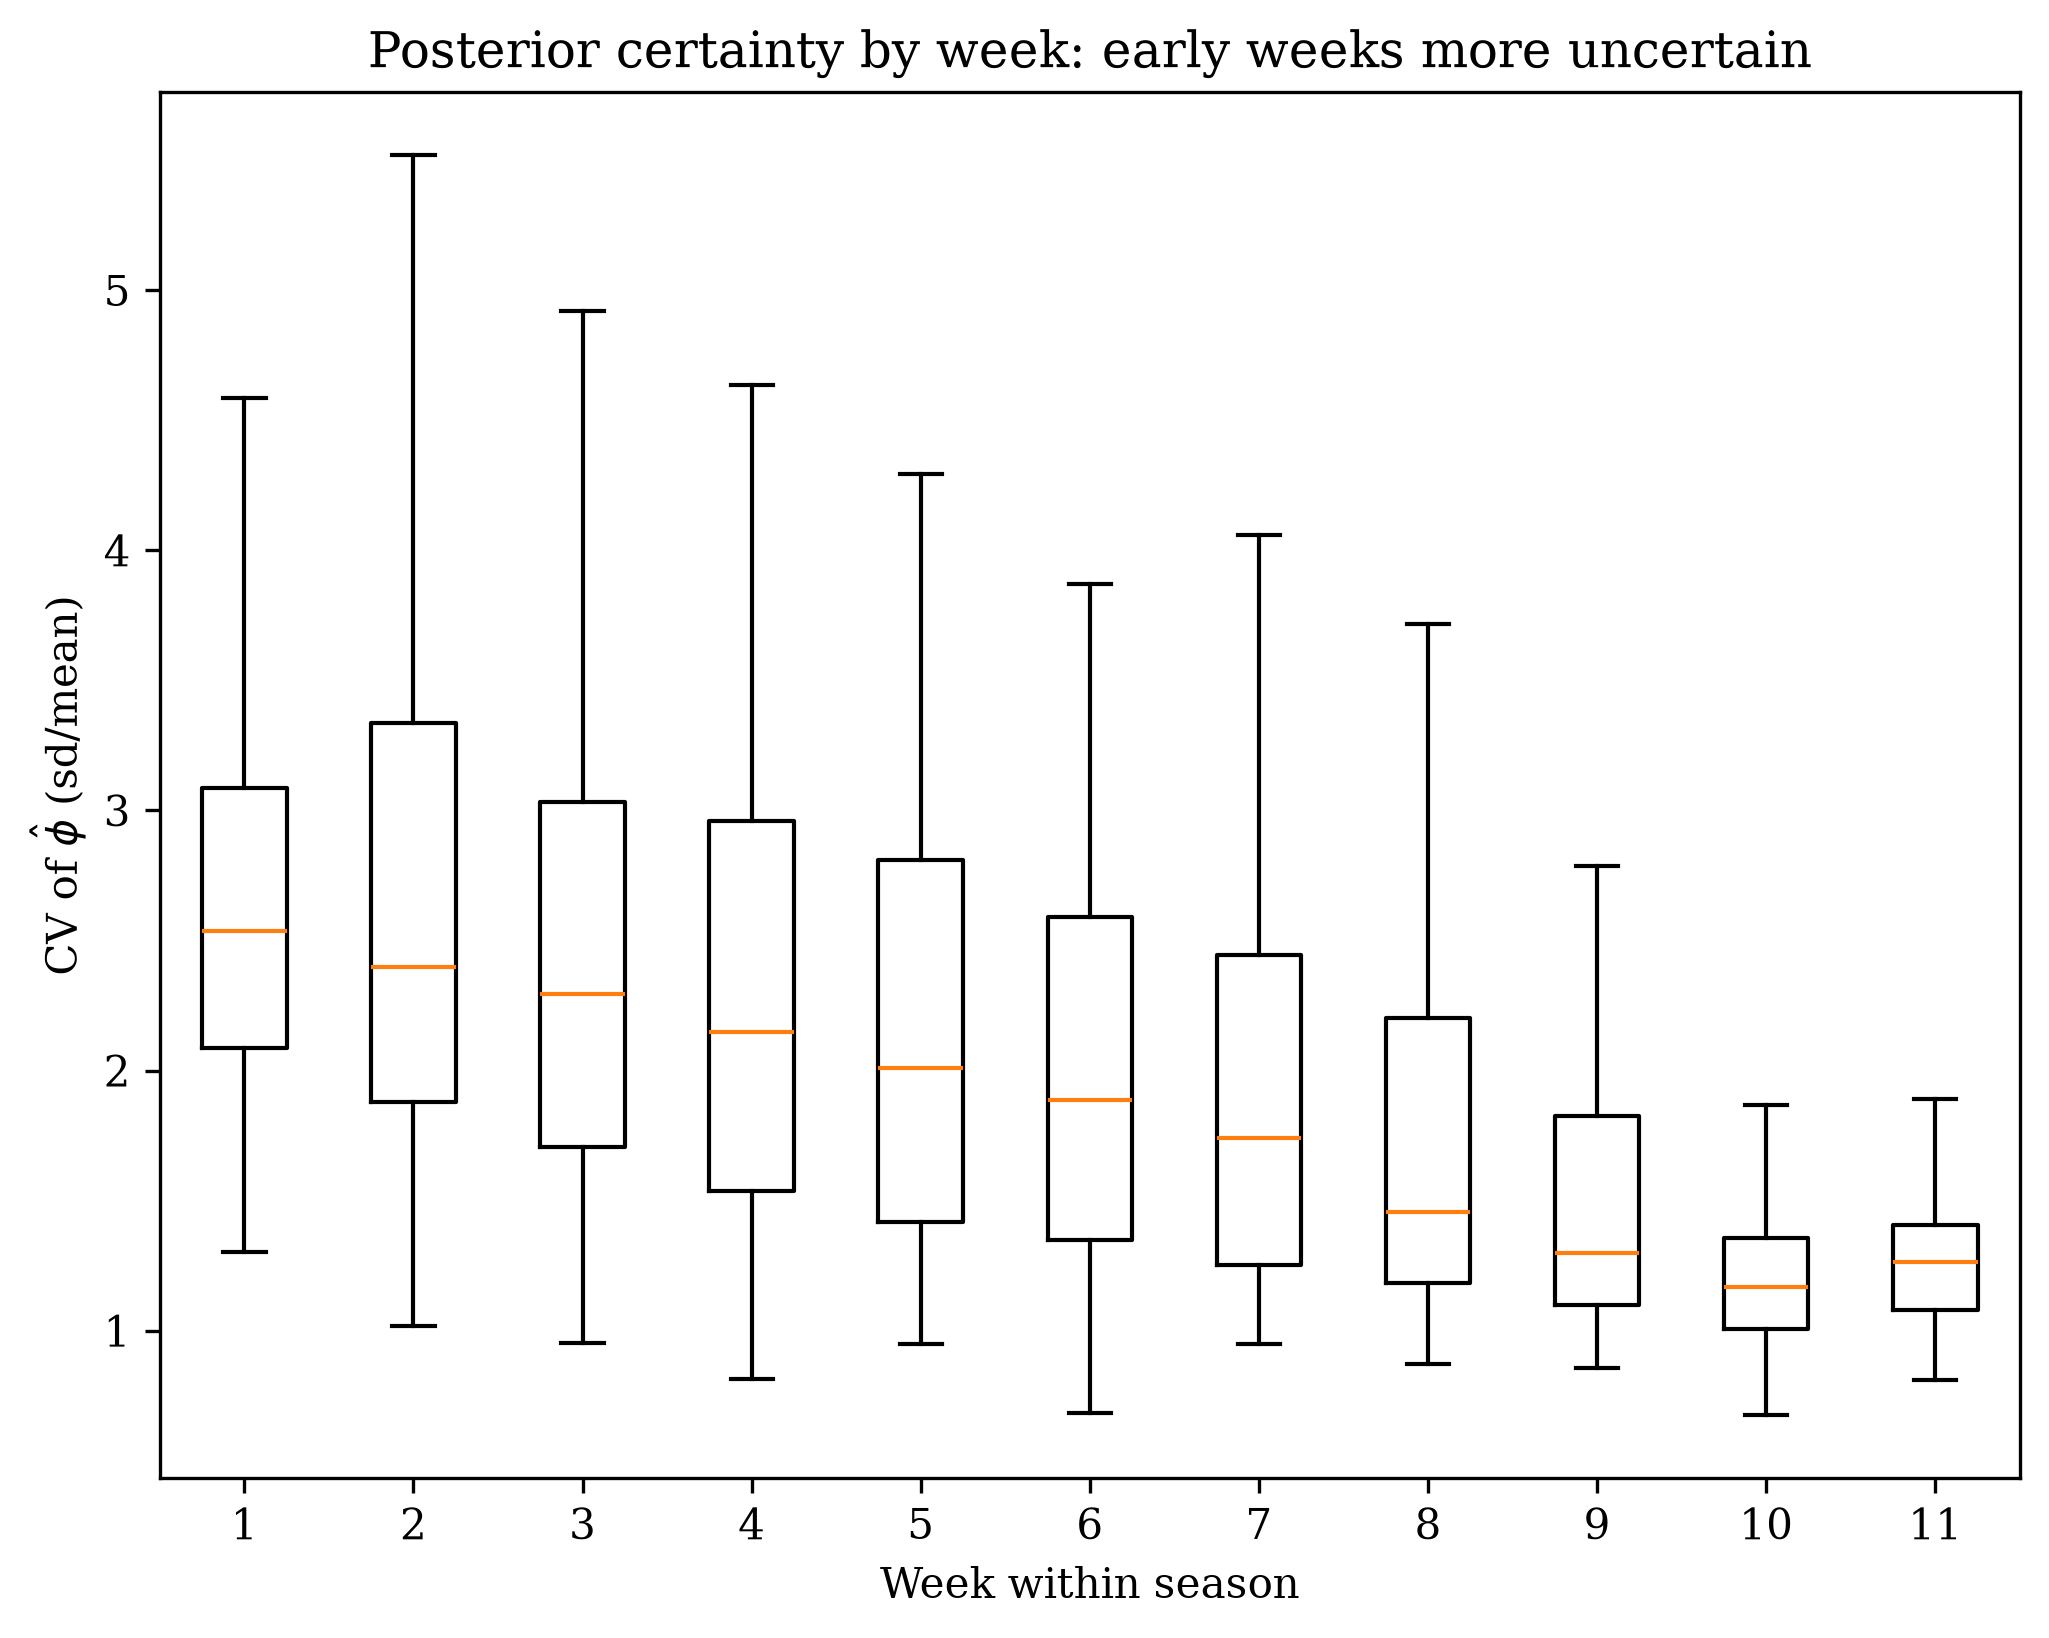
\includegraphics[width=0.8\textwidth]{model_1/figures/F4_cv_by_week.png}
\caption{Posterior CV of $\hat\phi$ by week-within-run: certainty increases as
eliminations accrete information.}
\label{fig:F4}
\end{figure}

Figure~\ref{fig:F4} quantifies certainty heterogeneity, the second explicit question
(``How much certainty is there in the fan vote totals you produced, and is that
certainty always the same for each contestant/week?''). CV falls from 2.72 (week-1
rows) to 2.23 (mid-run rows) as eliminations pin down the ordering information, so
certainty is materially \emph{not} constant across weeks or contestants.

\begin{figure}[H]
\centering
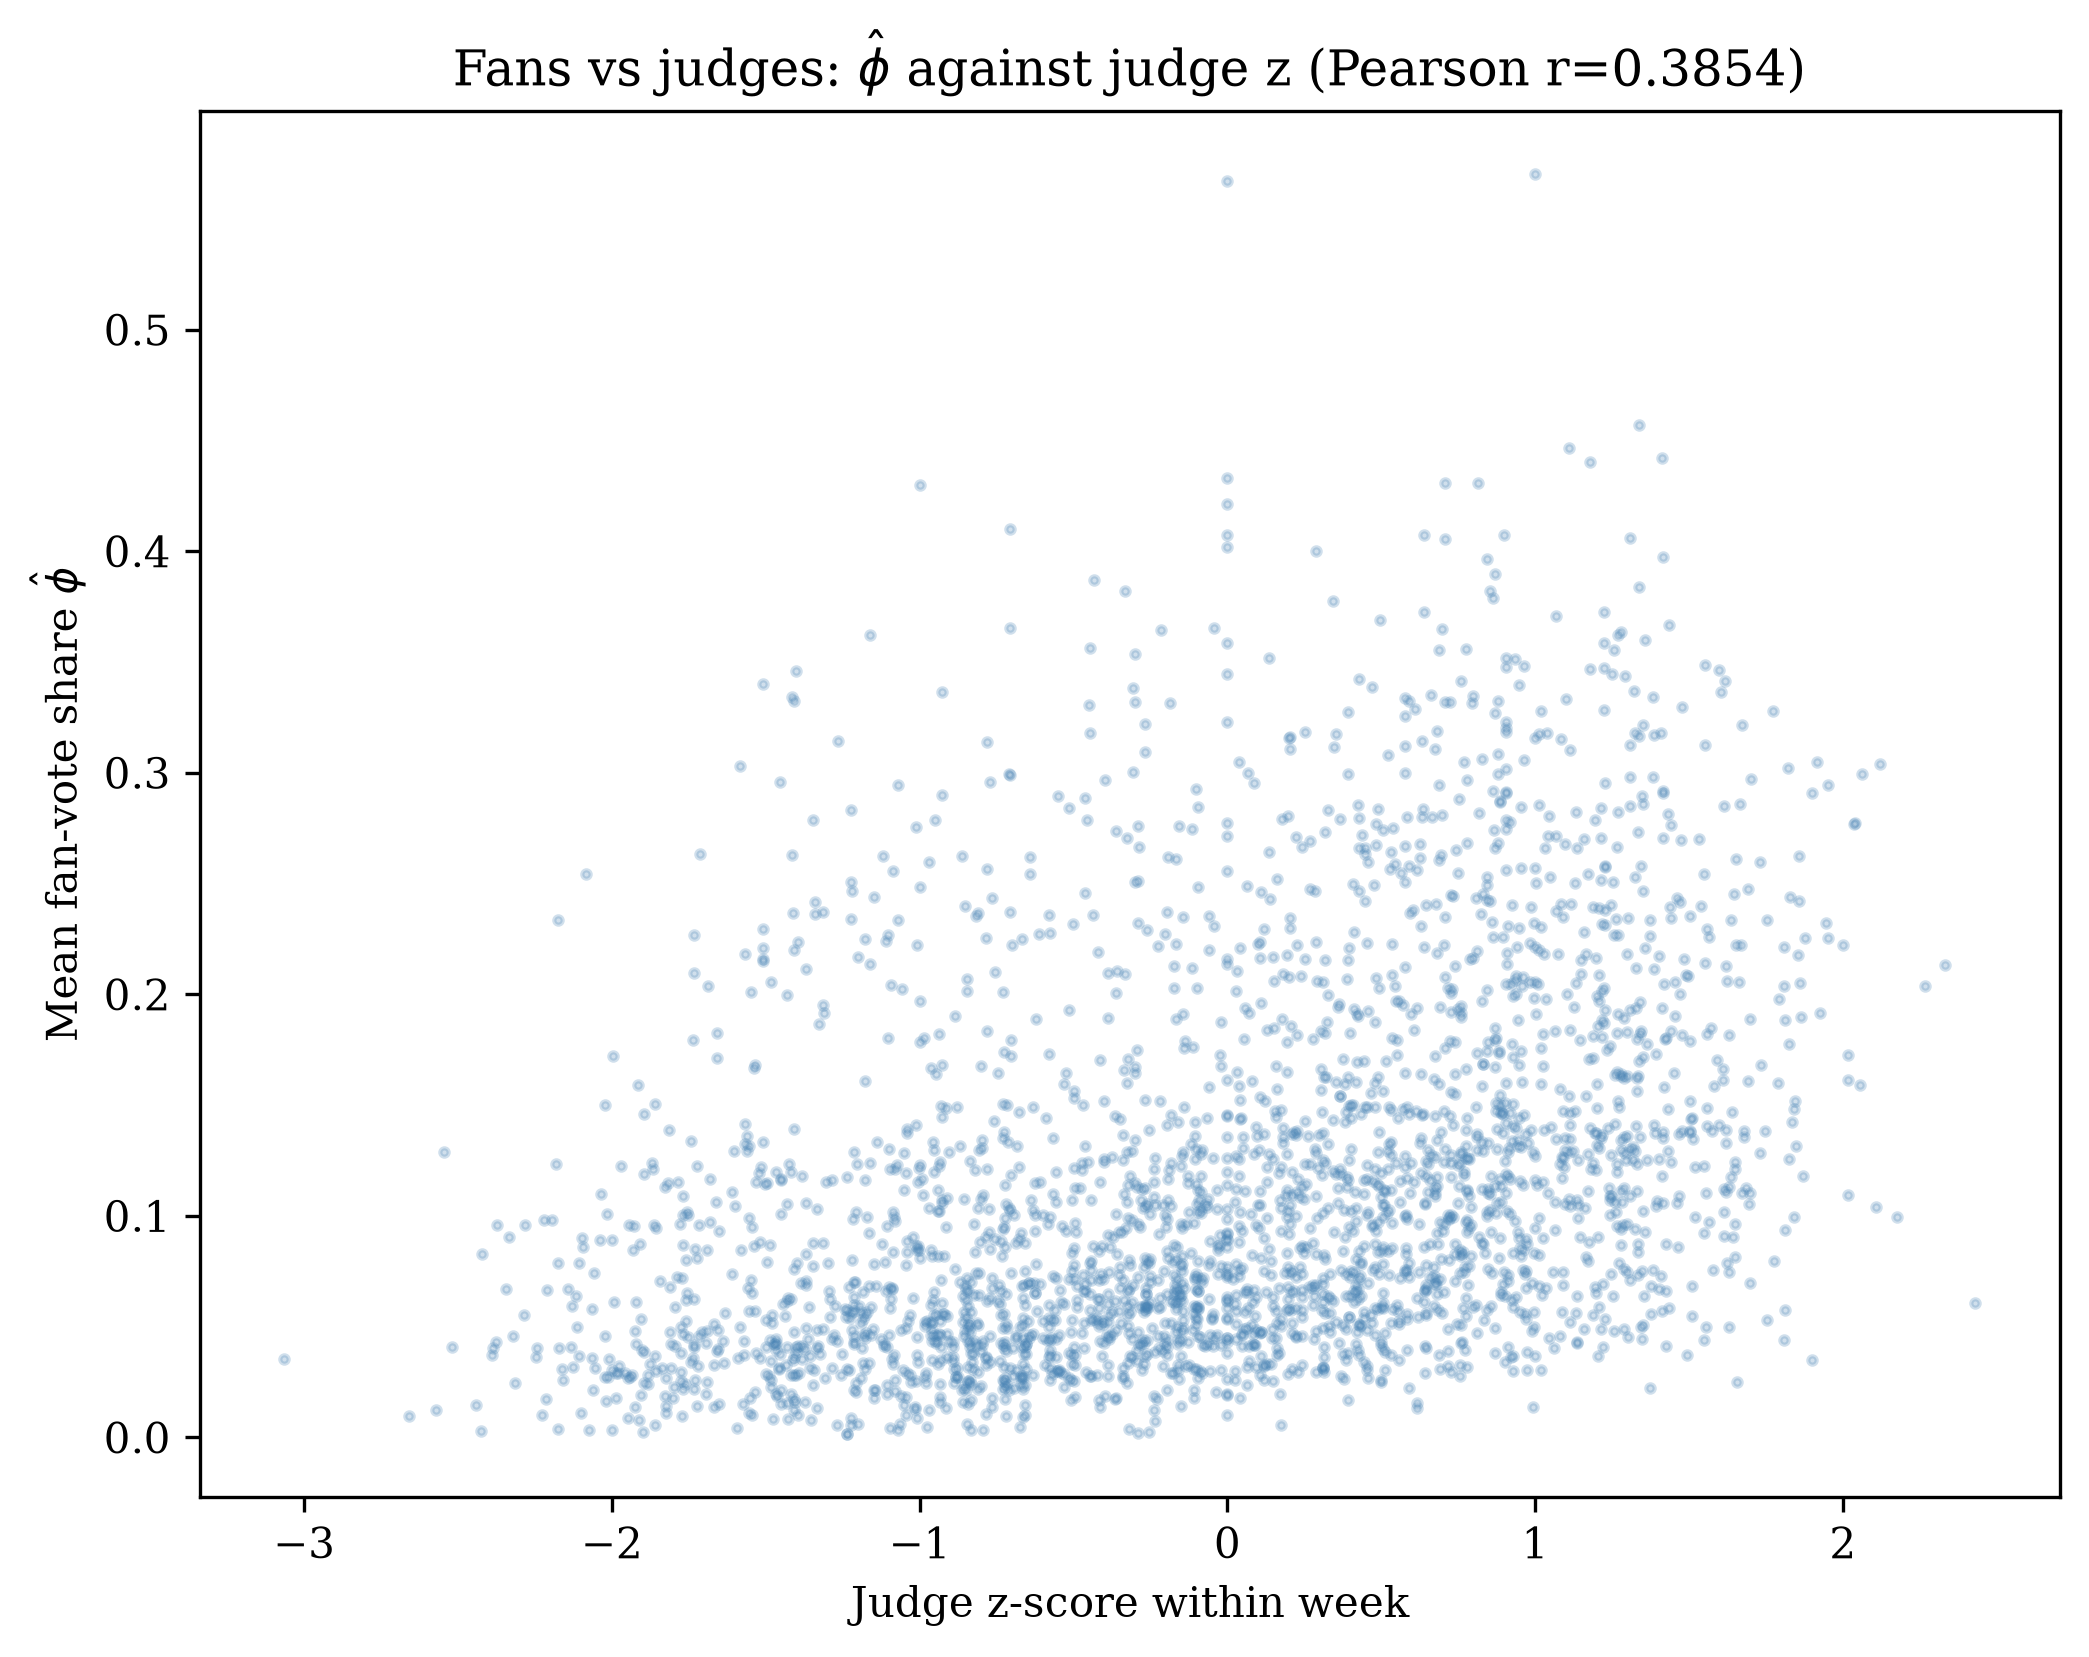
\includegraphics[width=0.8\textwidth]{model_1/figures/F5_phi_vs_judge_z.png}
\caption{Recovered $\hat\phi$ vs within-week judge z-score (corr.\ 0.397 on the
z-scale; 0.697 on the share scale): fans do not simply replicate judges.}
\label{fig:F5}
\end{figure}

\subsection{Validation}

Six pre-registered gates were tested: (1)\ exit recovery 100/100/100 as above;
(2)\ survivor identity exact on all 335 season-weeks; (3)\ coverage 1.00
(conservative) with the CV ratio 1.22 vs the 20\% gate; (4)\ leave-one-week-out
stability from 12 random exit weeks refit: Kendall $\tau$ with the full fit = 0.882
mean / 0.744 min season-scoped (gate $\ge 0.80$ met), 0.712 exit-week scoped;
(5)\ gradient correctness $\le 3\times10^{-8}$; (6)\ runtime seconds.

\subsection{Limitations}

(i)\ Ordinal-only identification: fan-share \emph{levels} are weakly identified
(median CV $\approx$ 1.0--2.7); rank \emph{orderings} are strongly identified.
(ii)\ 0/4{,}000 Laplace draws satisfy all 265 weekly ordinal facts exactly, so the
deliverable posterior keeps the least-violating quartile (1{,}000 draws),
exponential-weight ESS 2.33 --- $\phi\_sd$ is an upper bound on uncertainty.
(iii)\ Veto weeks model only bottom-2 membership. (iv)\ 13 repeat celebrities are
separate runs; judge positions are anonymous; multi-dance totals compared only
within-week.

\section{Model 2: Judge--Fan Behavioral Attribution}
\label{sec:model2}

\subsection{Problem Statement}

The third problem bullet asks how professional dancers and celebrity characteristics
(age, industry, etc.)\ influence performance, and \emph{whether they influence judge
scores and fan votes in the same way}. Judge scores are meant to reflect technical
merit, while fan votes respond to popularity and charisma --- so the two outcome
surfaces must be modeled \emph{separately} and their coefficient surfaces compared.
Model 2 consumes Model 1's posterior fan shares ($\hat\phi_{c,w}$, the canonical
input) alongside observed judge totals.

\subsection{Mathematical Formulation}

Two parallel linear response models share structure and differ only in the outcome:
\begin{equation}
y_{c,w} \;=\; \alpha_s \;+\; \pi_{p(c,s)} \;+\; \iota_{\text{ind}(c)} \;+\; f(\text{age}_c)
\;+\; g(w) \;+\; \theta\,\text{multi}_{c,w} \;+\; \epsilon_{c,w},
\label{eq:m2}
\end{equation}
where the judge surface is $y^J_{c,w} = z(x_{c,w})$ (within-week, dance-count aware)
and the fan surface is $y^F_{c,w} = \text{logit}(\hat\phi_{c,w} + \delta)$ with a
small offset $\delta$. The design comprises intercept $+$ 33 season dummies $+$ 52
professional-dancer indicators (drop-first coding; reference = Alan Bersten) $+$ 25
industry indicators (reference = Actor/Actress) $+$ restricted cubic splines for age
(knots at 20/30/45/65) and week-within-run (knots at 1/3/6/10) $+$ a multi-dance
flag: 116 parameters on 2{,}777 rows.

The headline statistic is the \emph{variance decomposition}
$R_k = \text{partial R}^2$ attributable to covariate block $k \in \{\text{pro},
\text{industry}, \text{age}, \text{week}, \text{multi}, \text{season}\}$, computed
on both surfaces and tested by permutation (1{,}000 shuffles of the block, re-using
the identical drop-first coding and column order; run-level attributes shuffle
across runs within season, week shuffles within run).

\paragraph{Anti-sorting control.} Pro-dancer assignments are not random --- producers
assign pros partly by celebrity caliber. We therefore re-fit on weeks 2+ with the
couple's week-1 fan-logit (an entry-fame proxy) as a control: the restricted
$R^{\text{pro}}$ is the honest lower bound on the pro effect.

\subsection{Implementation}

Python; OLS with celebrity-run cluster-robust standard errors (421 clusters),
\texttt{statsmodels}; 1{,}000-permutation nulls; 2{,}000 cluster-bootstraps for effect
CIs. Fan-side blocks use the canonical Model 1 input; an in-house identification
stage (``Model-1-lite'', $\hat\beta = 1.387$ judge coupling, MAP nll 436.58) is
retained as a sensitivity column \texttt{fanshare\_lite}. Deviations from the master
plan, reported for transparency: OLS with cluster-robust SEs replaces the PyMC
hierarchical spec (identical functional form), and the pro $\times$ industry
interaction is dropped (sparse cells in the $25 \times 52$ design).

\subsection{Results}

\begin{table}[H]
\centering
\caption{Variance decomposition $R_k$ (partial R\textsuperscript{2}) by surface,
with permutation $p$-values (1{,}000 shuffles).}
\label{tab:m2decomp}
\small
\begin{tabular}{lcccc}
\toprule
Block & Judge surface & $p$ & Fan surface & $p$ \\
\midrule
Professional dancer & 0.125 & 0.003 & 0.138 & 0.090 \\
Industry & 0.059 & 0.028 & 0.056 & 0.481 \\
Age (spline) & 0.134 & 0.001 & 0.094 & 0.001 \\
Week-within-run & 0.018 & 0.099 & 0.164 & 0.001 \\
Multi-dance flag & $\approx 0$ & --- & $\approx 0$ & --- \\
Season & 0.018 & --- & 0.095 & --- \\
\midrule
Surface R\textsuperscript{2} & \multicolumn{2}{c}{0.336} & \multicolumn{2}{c}{0.392} \\
\bottomrule
\end{tabular}
\end{table}

\textbf{Do pros matter? Yes, on both surfaces, but differently.} The pro block
explains $R = 0.125$ of judge-score variance (permutation $p = 0.003$; our $R$
exceeds the permuted 95th percentile 0.106) and $R = 0.138$ of fan-share variance
($p = 0.090$). The age block is the strongest single judge-surface driver (0.134,
$p=0.001$), while \emph{week-within-run} dominates the fan surface (0.164, $p =
0.001$ vs 0.018 on judges, $p=0.099$): fans reward within-run momentum far more
than judges do. Industry matters modestly (0.059 judge; $p = 0.028$) and is
indistinguishable from noise on the fan surface ($p = 0.481$).

\textbf{Known-elite validation.} Among the 41 eligible pros ($\ge 2$ seasons),
Derek Hough ranks \#1 on the judge surface ($+0.662$, 95\% CI $[0.447, 0.942]$),
followed by Artem Chigvintsev ($+0.392$), Valentin Chmerkovskiy \#3 ($+0.280$),
Corky Ballas ($+0.255$), and Mark Ballas \#5 ($+0.188$); Cheryl Burke is \#15
($+0.056$). All four named known-elite pros land inside the top-15 validation
gate. On the fan surface the top five are Derek Hough ($+0.534$), Daniella
Karagach ($+0.402$), Kym Johnson ($+0.322$), Jenna Johnson ($+0.320$), and Val
Chmerkovskiy ($+0.308$).

\textbf{Same direction --- but far from collinear.} Judge- and fan-effect point
estimates correlate at $\rho = 0.623$ across eligible pros ($0.472$ incl.\ all 52):
pros who lift judges tend to lift fans, yet there are material disagreements.
Daniella Karagach and Jenna Johnson are top-4 on fans while \emph{negative} on
judges; Artem Chigvintsev, \#2 on judges, is fan-neutral ($-0.102$). This positive-
but-imperfect alignment is exactly the ``do they impact both in the same way?''
answer: same broad direction, different magnitudes, several striking exceptions.

\textbf{Sorting honesty.} The week-1 fame control absorbs almost the entire raw
fan-side association ($R_{\text{fame}} = 0.717$ on weeks 2+), while on the judge
surface the naive $R^{\text{pro}} = 0.128$ drops to $0.114$ restricted: only
$\sim$11\% of the raw judge-side association is producer sorting. The honest reading:
the fan-support premium of star pros is largely an \emph{entry-popularity} effect,
whereas the judge-side pro effect survives the control nearly intact.

\textbf{Age.} The restricted-cubic-spline curve (reference age 36) declines from
$-0.27$ (age 20) to $-0.97$ (44), $-1.61$ (62), and $-2.15$ (82) on the judge
surface, with a fan-side plateau ($-1.26$ at 82 vs $-1.17$ at 62): older celebrities
lose judges faster than fans --- the charm-compensation effect. A sign-discipline
flag, reported honestly: the judge age curve is \emph{negative} at age 20
($-0.27$), violating the pre-registered assumption of non-negativity on [15, 45];
judge favorability actually peaks near ages 40--45. This mirrors the week-curve
finding (experience vs.\ flexibility) rather than indicating a coding bug.

\textbf{Learning curve.} Absolute judge scores rise within runs ($+1.52$ points,
$p < 10^{-6}$, 326 runs with $\ge 4$ weeks) while the within-week relative z-score
\emph{falls} ($-0.47$, $p < 10^{-6}$) --- survivorship composition, not decline:
remaining castmates improve as fast as the survivor. On the fan surface, the
logit share rises $+0.115$ ($p = 0.0007$): fans reward improvement.

\textbf{Era drift.} Splitting the sample (S1--17 / S18--27 / S28--34), the mean
within-week fan--judge Spearman correlation drifts $0.539 \to 0.510 \to 0.465$ and
the mean $|$fan$-$judge$|$ share gap narrows $0.052 \to 0.055 \to 0.043$. The
post-2023 (S28+) reform era did \emph{not} re-align fans with judges; rankings
diverged more while staying equally informative (84.3\% bottom-$m$ exit
recovery), and the median top/bottom share ratio remains 6.0--7.3$\times$.

\textbf{Counterfactual pro swap.} For a median celebrity (season 10 baseline,
age 36, Actor/Actress, week 5), pairing with Derek Hough predicts judge-z $+0.672$
and fan share 16.9\%; with Peta Murgatroyd (median) $-0.081$ and 10.6\%; with Koko
Iwasaki (worst eligible) $-1.505$ and 4.3\%. The partnership alone is worth
$\approx$ 2.2 judge-z units and $\approx$ 12.5 percentage points of weekly fan
share between best and worst pairing.

Industry extremes (25 levels): judge-surface top = Producer ($+1.019$, single run)
and Astronaut ($+0.817$); bottom = Con artist ($-1.245$) and Politician
($-0.964$). Fan-surface top = Musician ($+1.034$); bottom = Con artist ($-2.045$).

\subsection{Figures}

\begin{figure}[H]
\centering
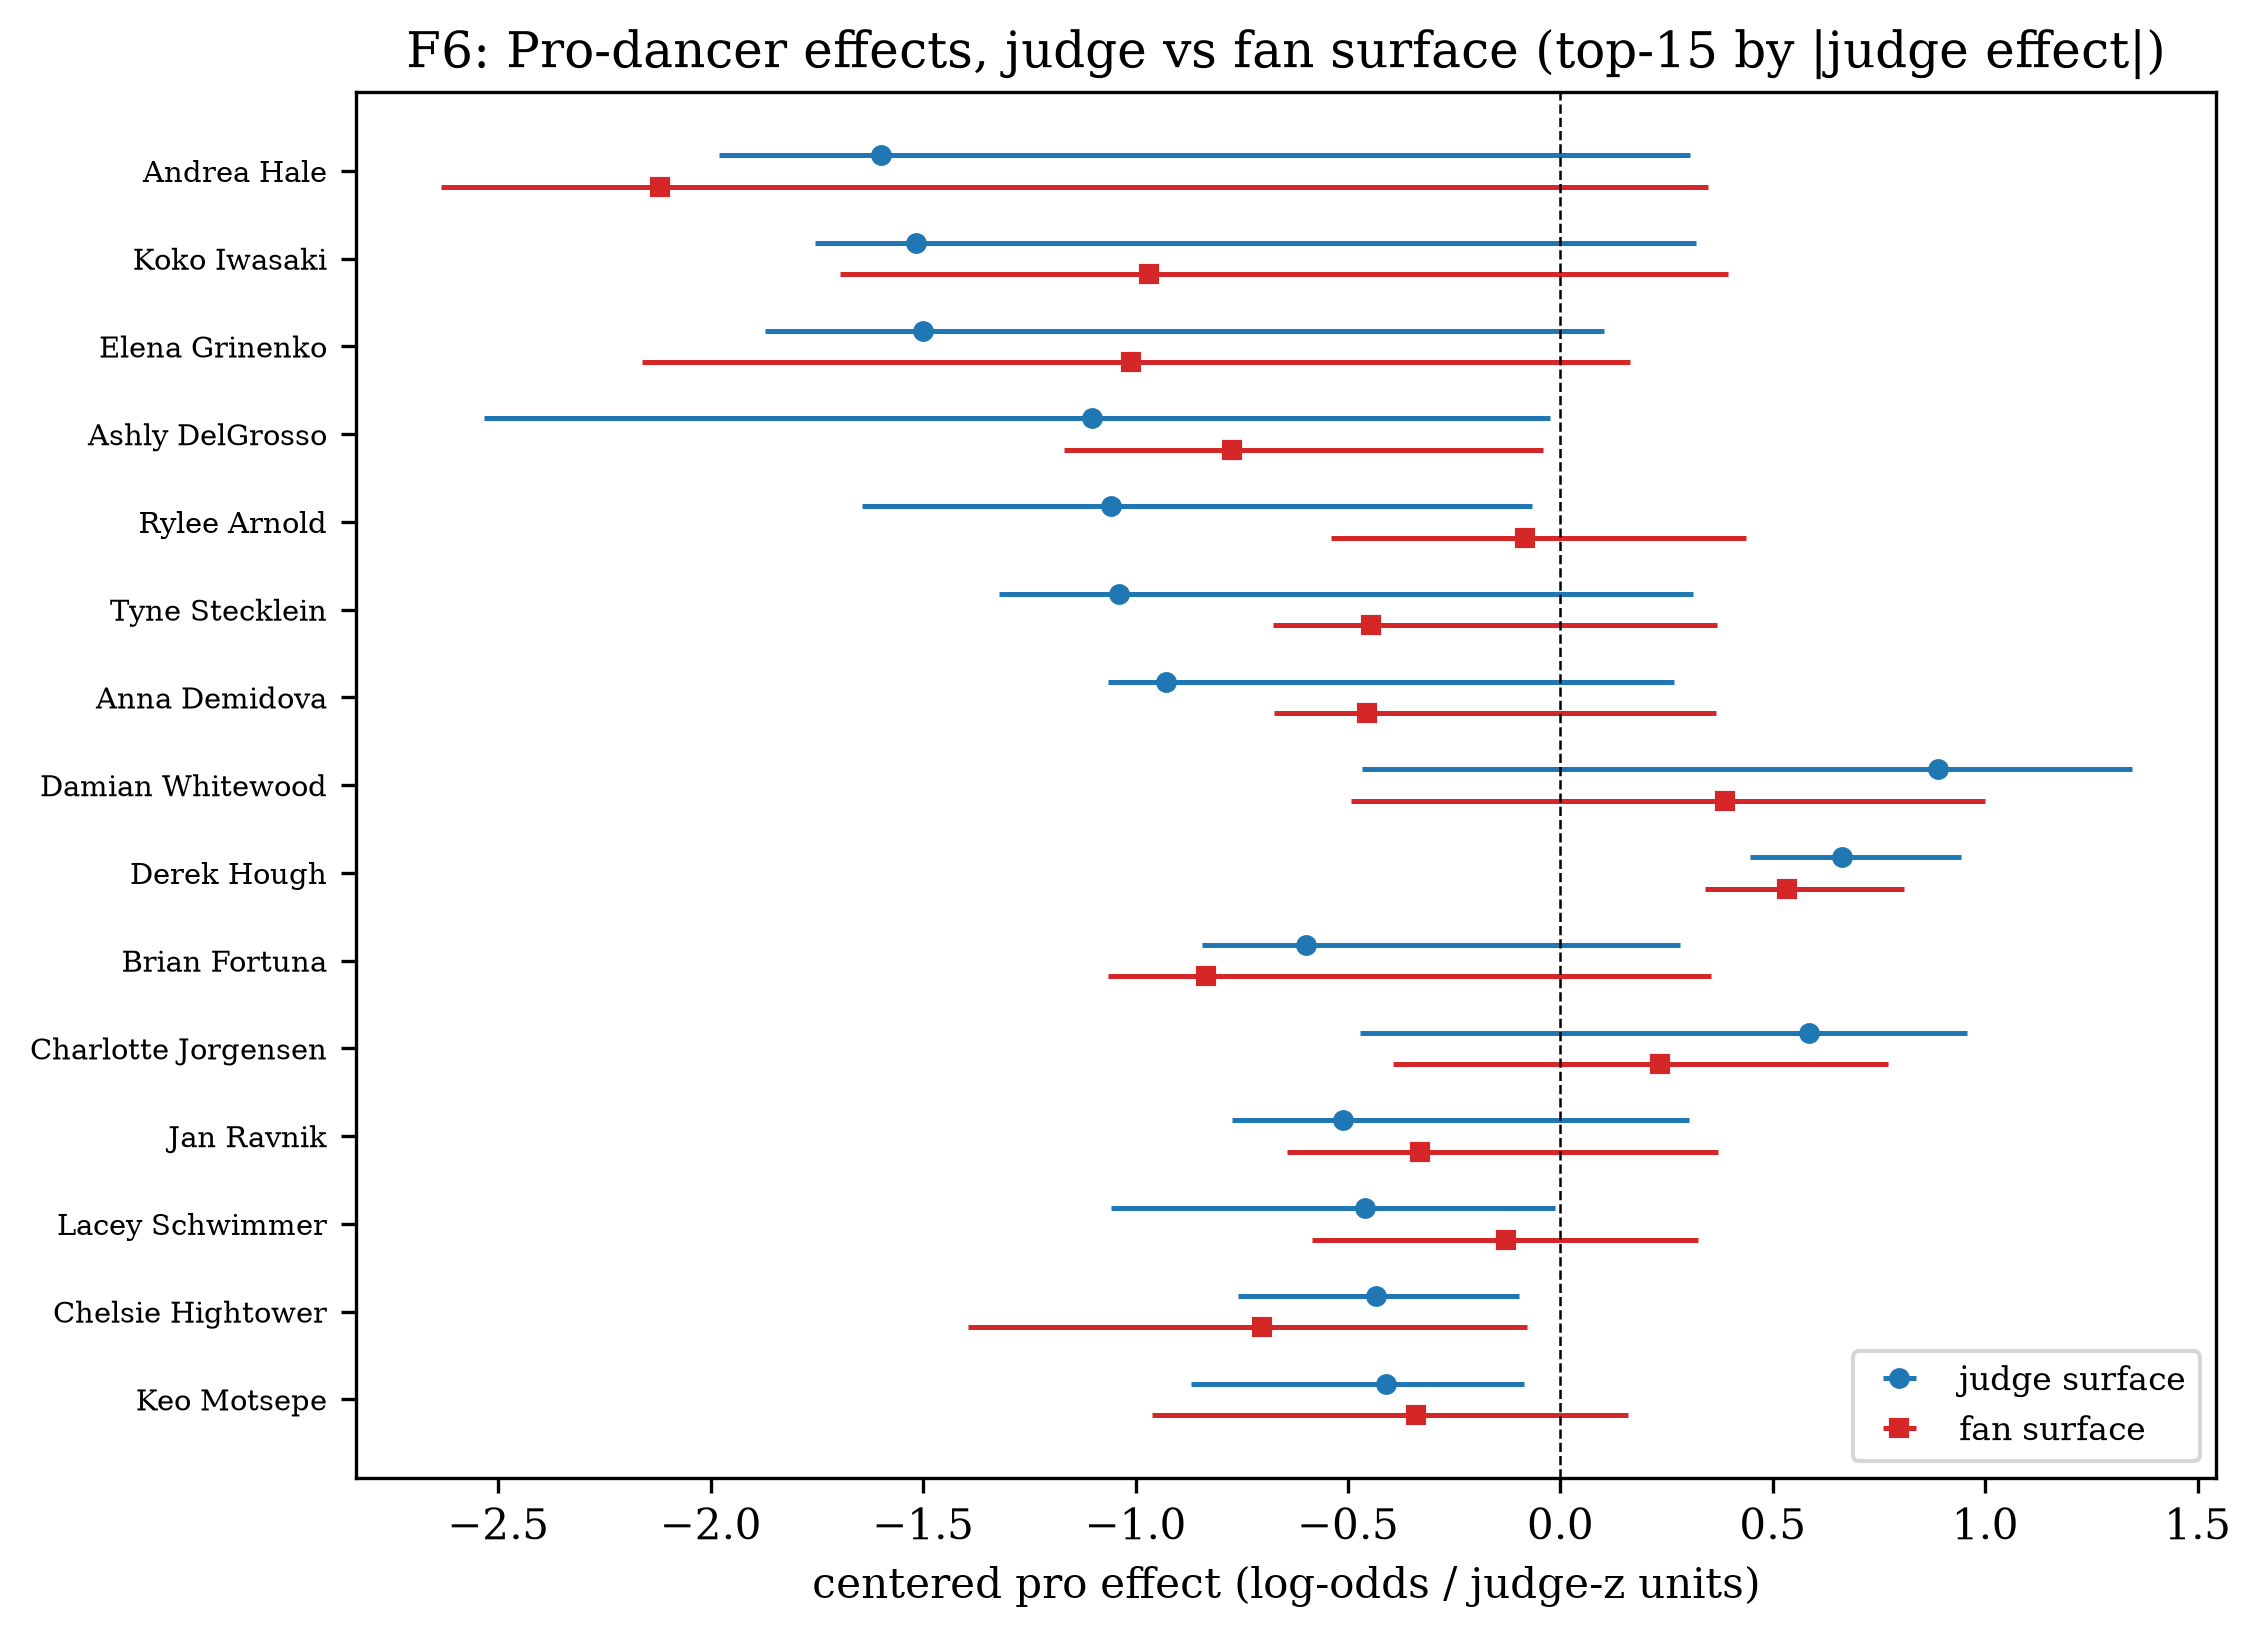
\includegraphics[width=0.85\textwidth]{model_2/figures/F6_pro_forest.png}
\caption{Top-15 pro effects (eligible pros), judge vs fan surface, with 95\%
cluster-bootstrap CIs.}
\label{fig:F6}
\end{figure}

Figure~\ref{fig:F6} shows the paired forest plot. Derek Hough dominates both
surfaces; the fan-judge discrepancies for Daniella Karagach and Jenna Johnson
(positive fan, negative judge) are visible as discordant intervals.

\begin{figure}[H]
\centering
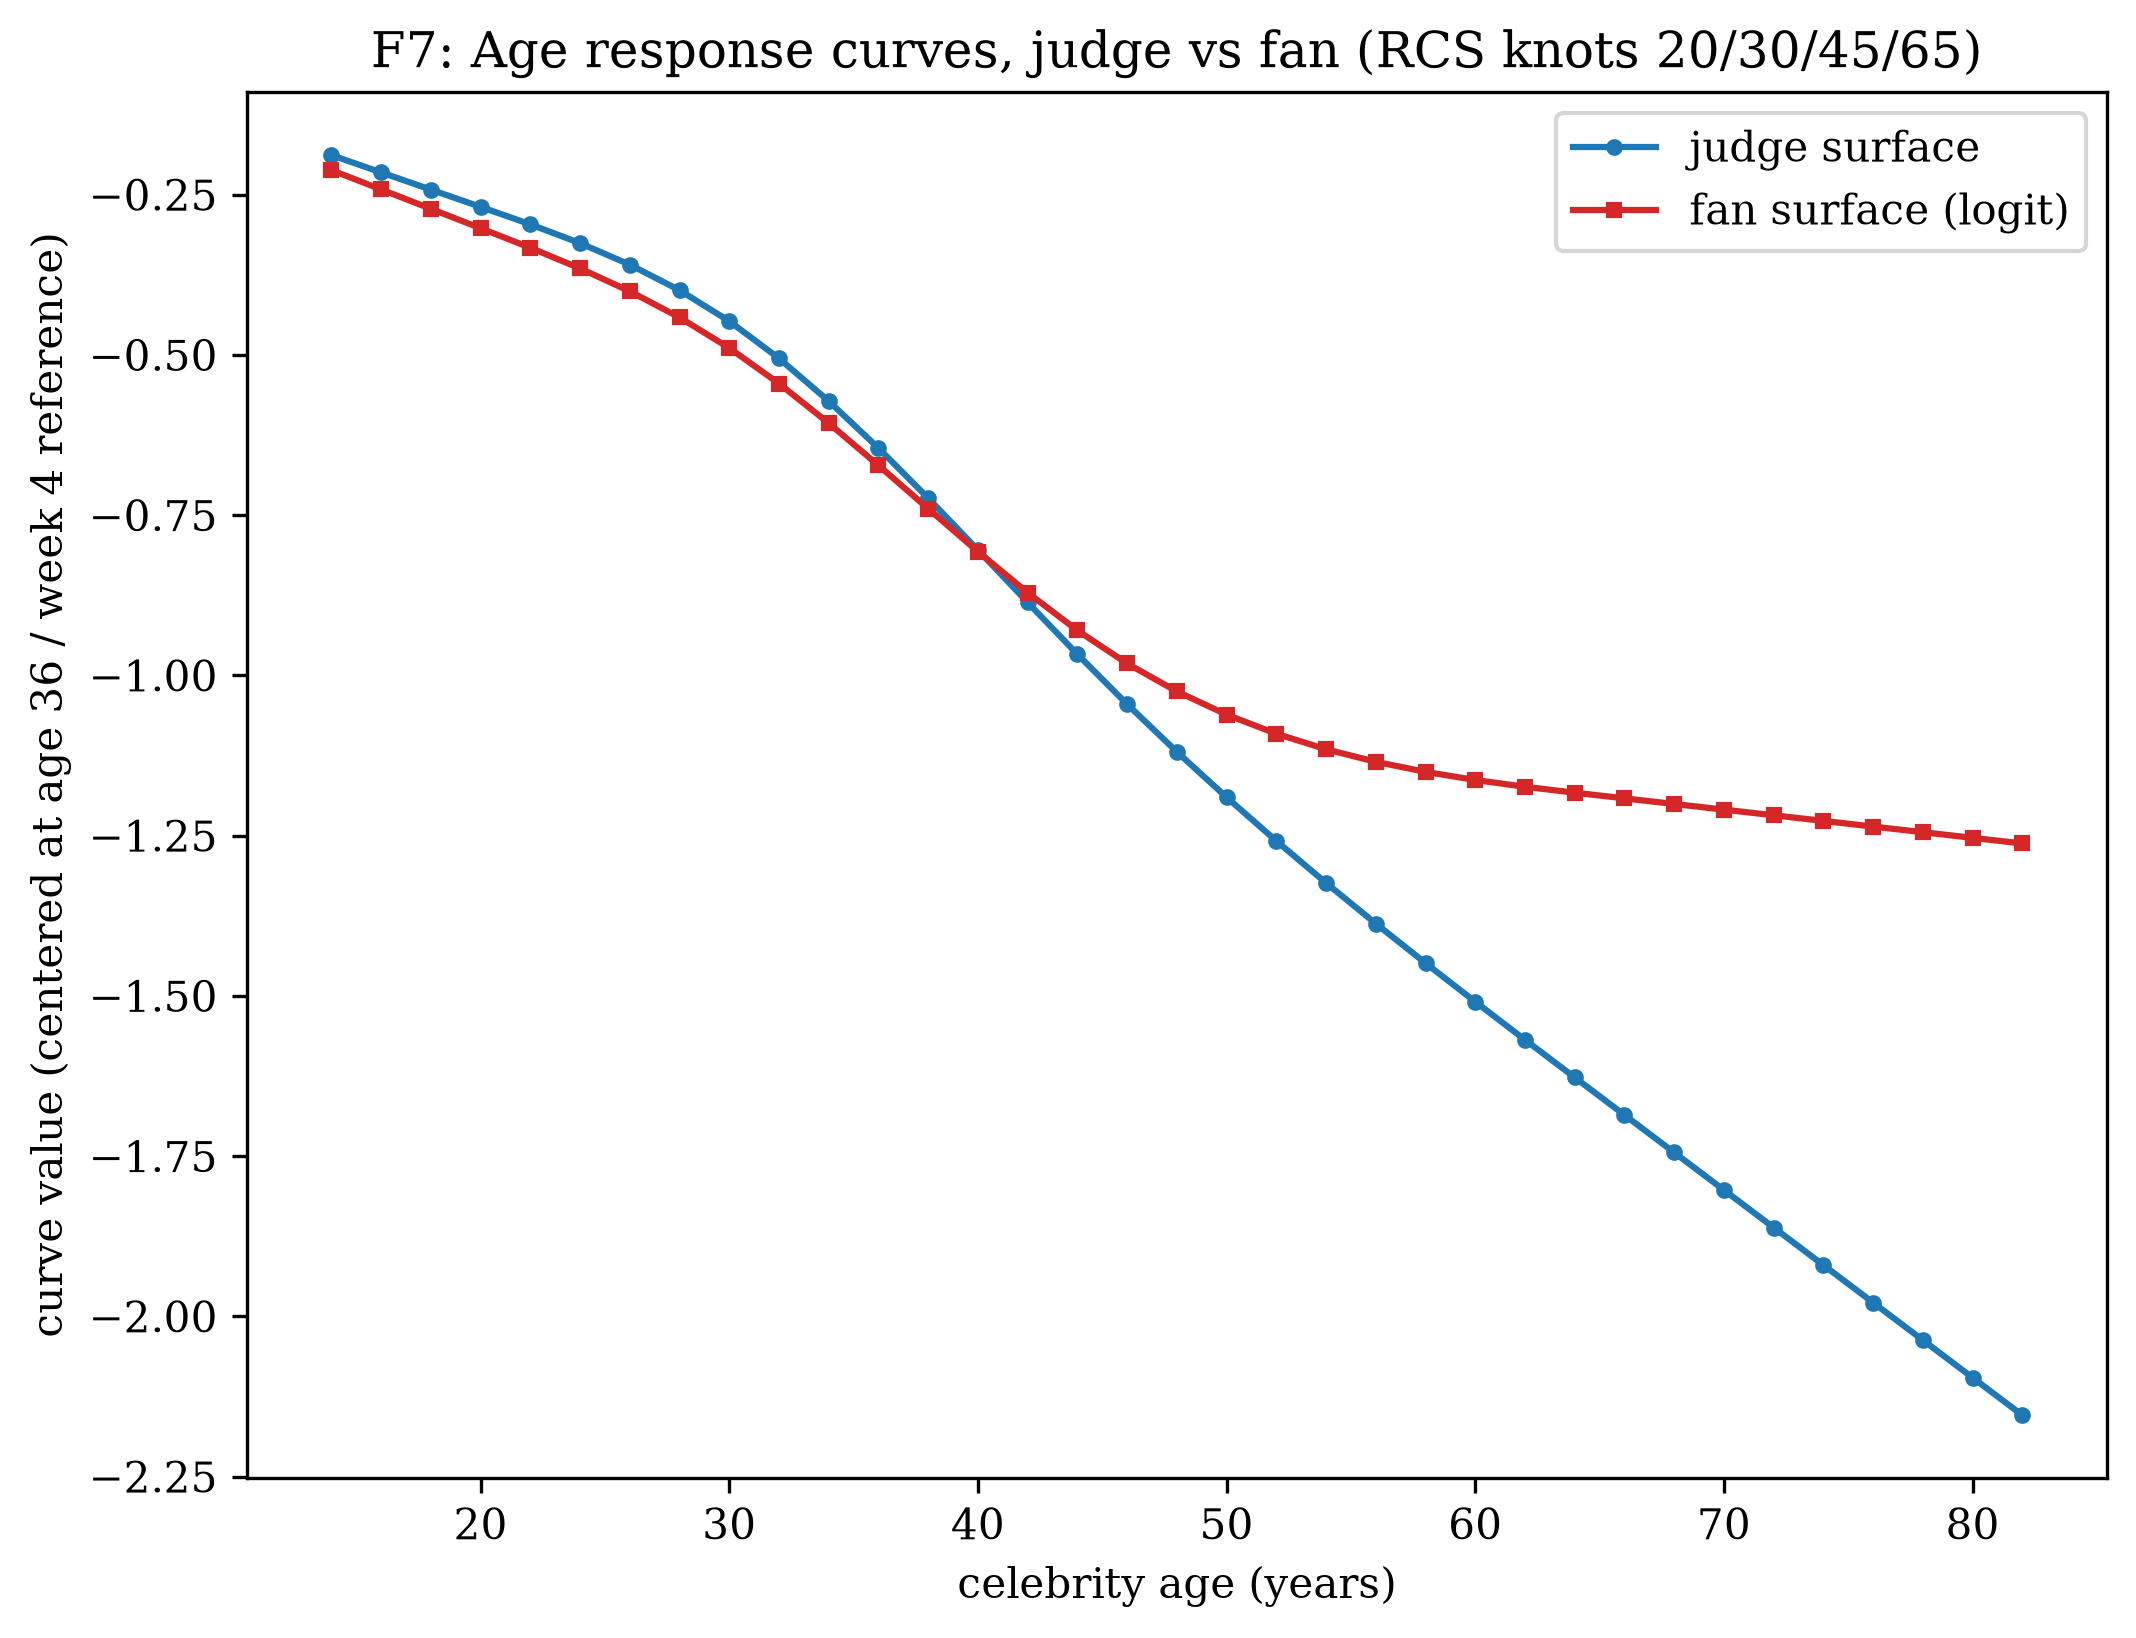
\includegraphics[width=0.75\textwidth]{model_2/figures/F7_age_spline.png}
\caption{Age response curves (RCS knots 20/30/45/65), judge vs fan surfaces.}
\label{fig:F7}
\end{figure}

Figure~\ref{fig:F7} shows near-monotone decline with age on both surfaces, with the
fan curve flattening late --- old celebrities keep fan support longer than judge
support.

\begin{figure}[H]
\centering
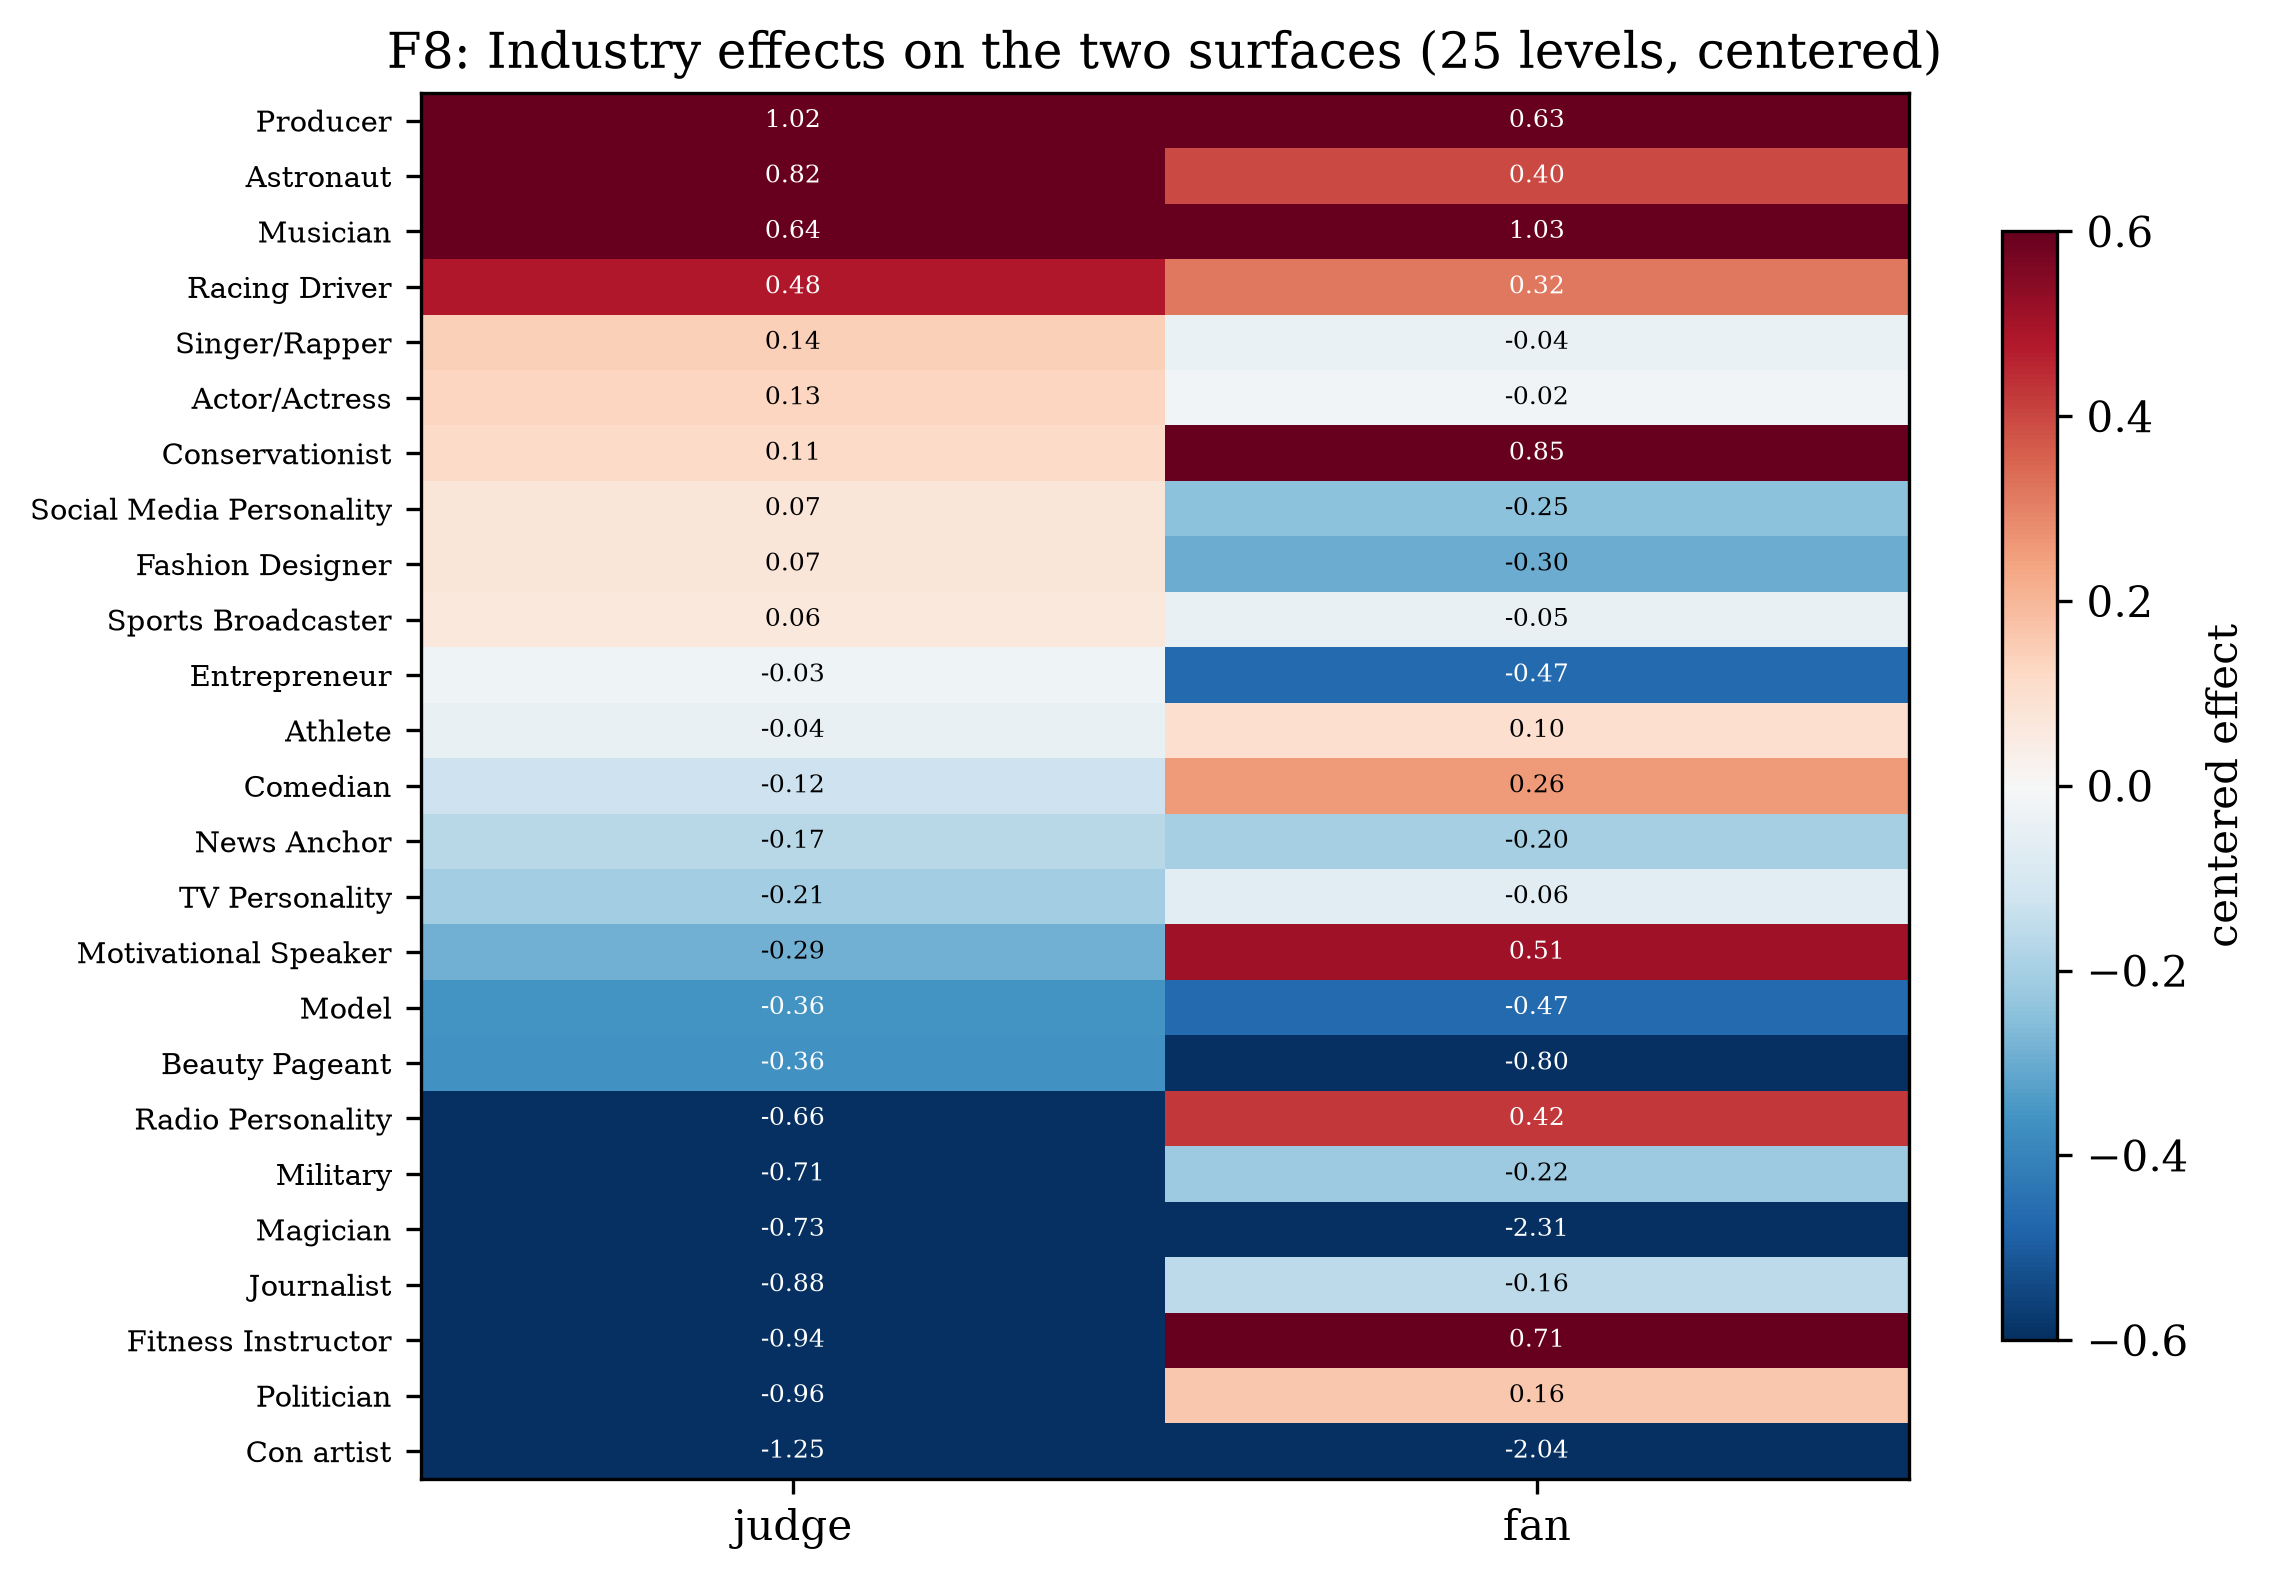
\includegraphics[width=0.85\textwidth]{model_2/figures/F8_industry_heatmap.png}
\caption{Centered industry effects (25 levels $\times$ 2 surfaces).}
\label{fig:F8}
\end{figure}

\begin{figure}[H]
\centering
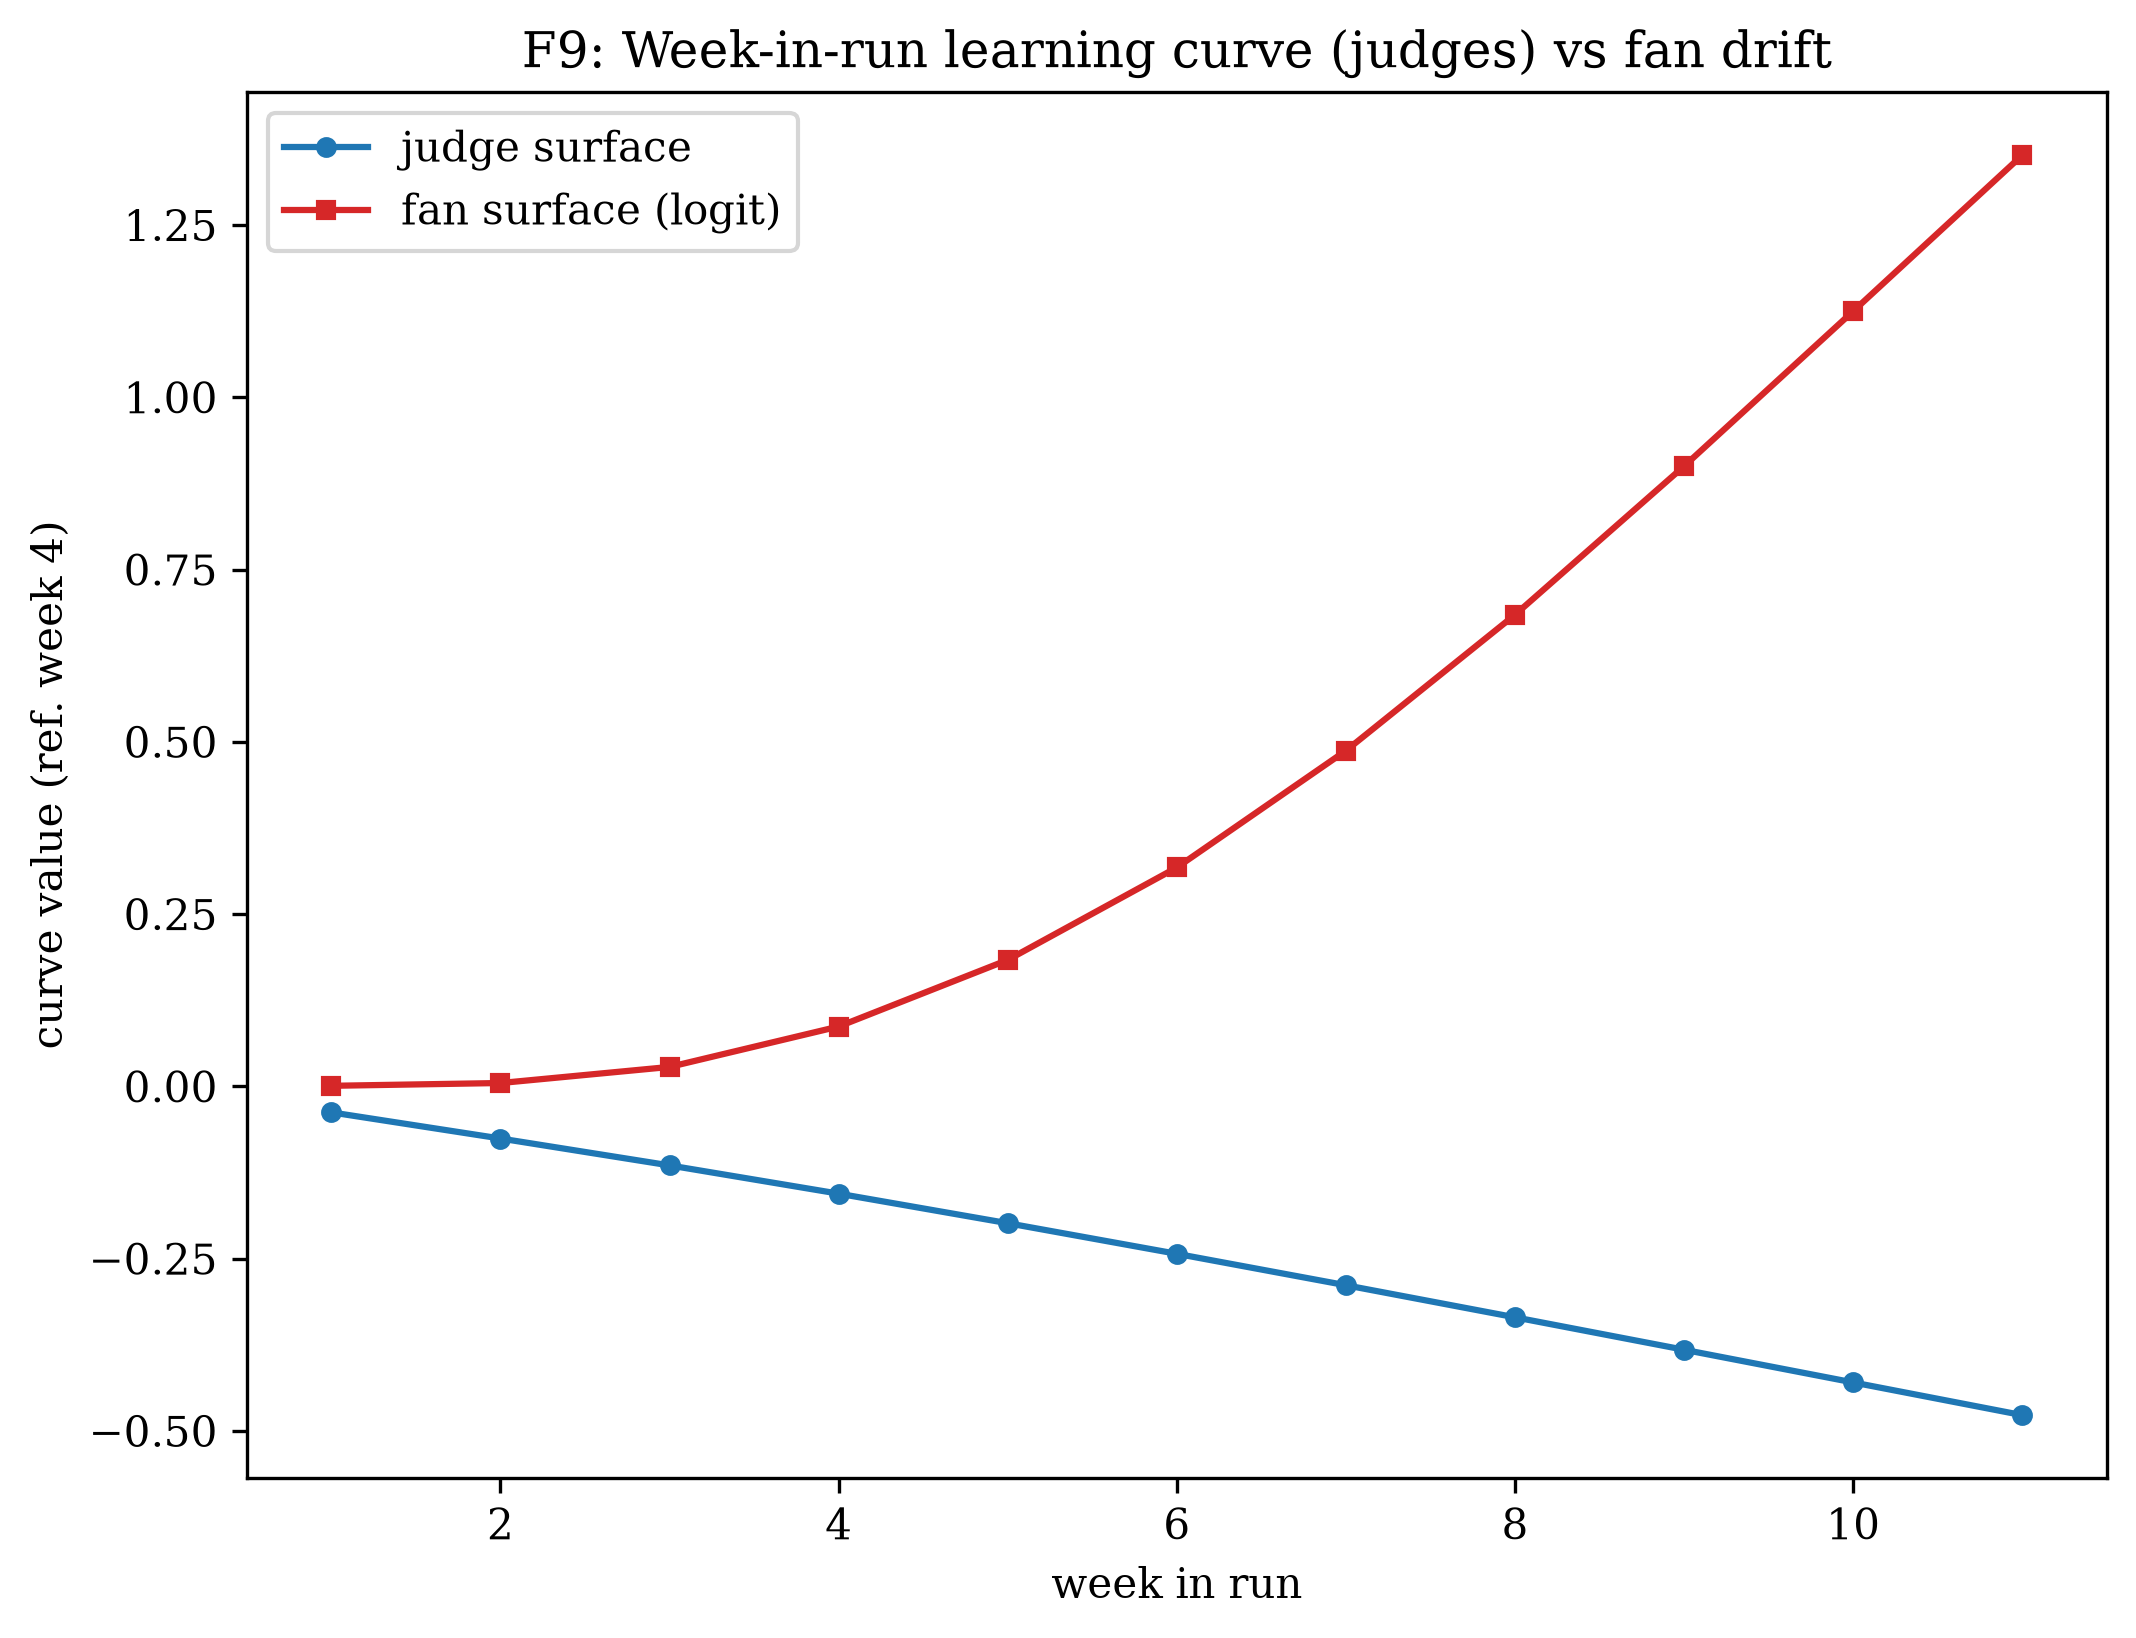
\includegraphics[width=0.75\textwidth]{model_2/figures/F9_week_curve.png}
\caption{Week-within-run response, judge vs fan surfaces.}
\label{fig:F9}
\end{figure}

Figure~\ref{fig:F9} contrasts the two audiences' time profiles: judges' relative
position drifts down within a run (survivorship composition), while fan logit share
rises steadily --- fans reward visible improvement.

\begin{figure}[H]
\centering
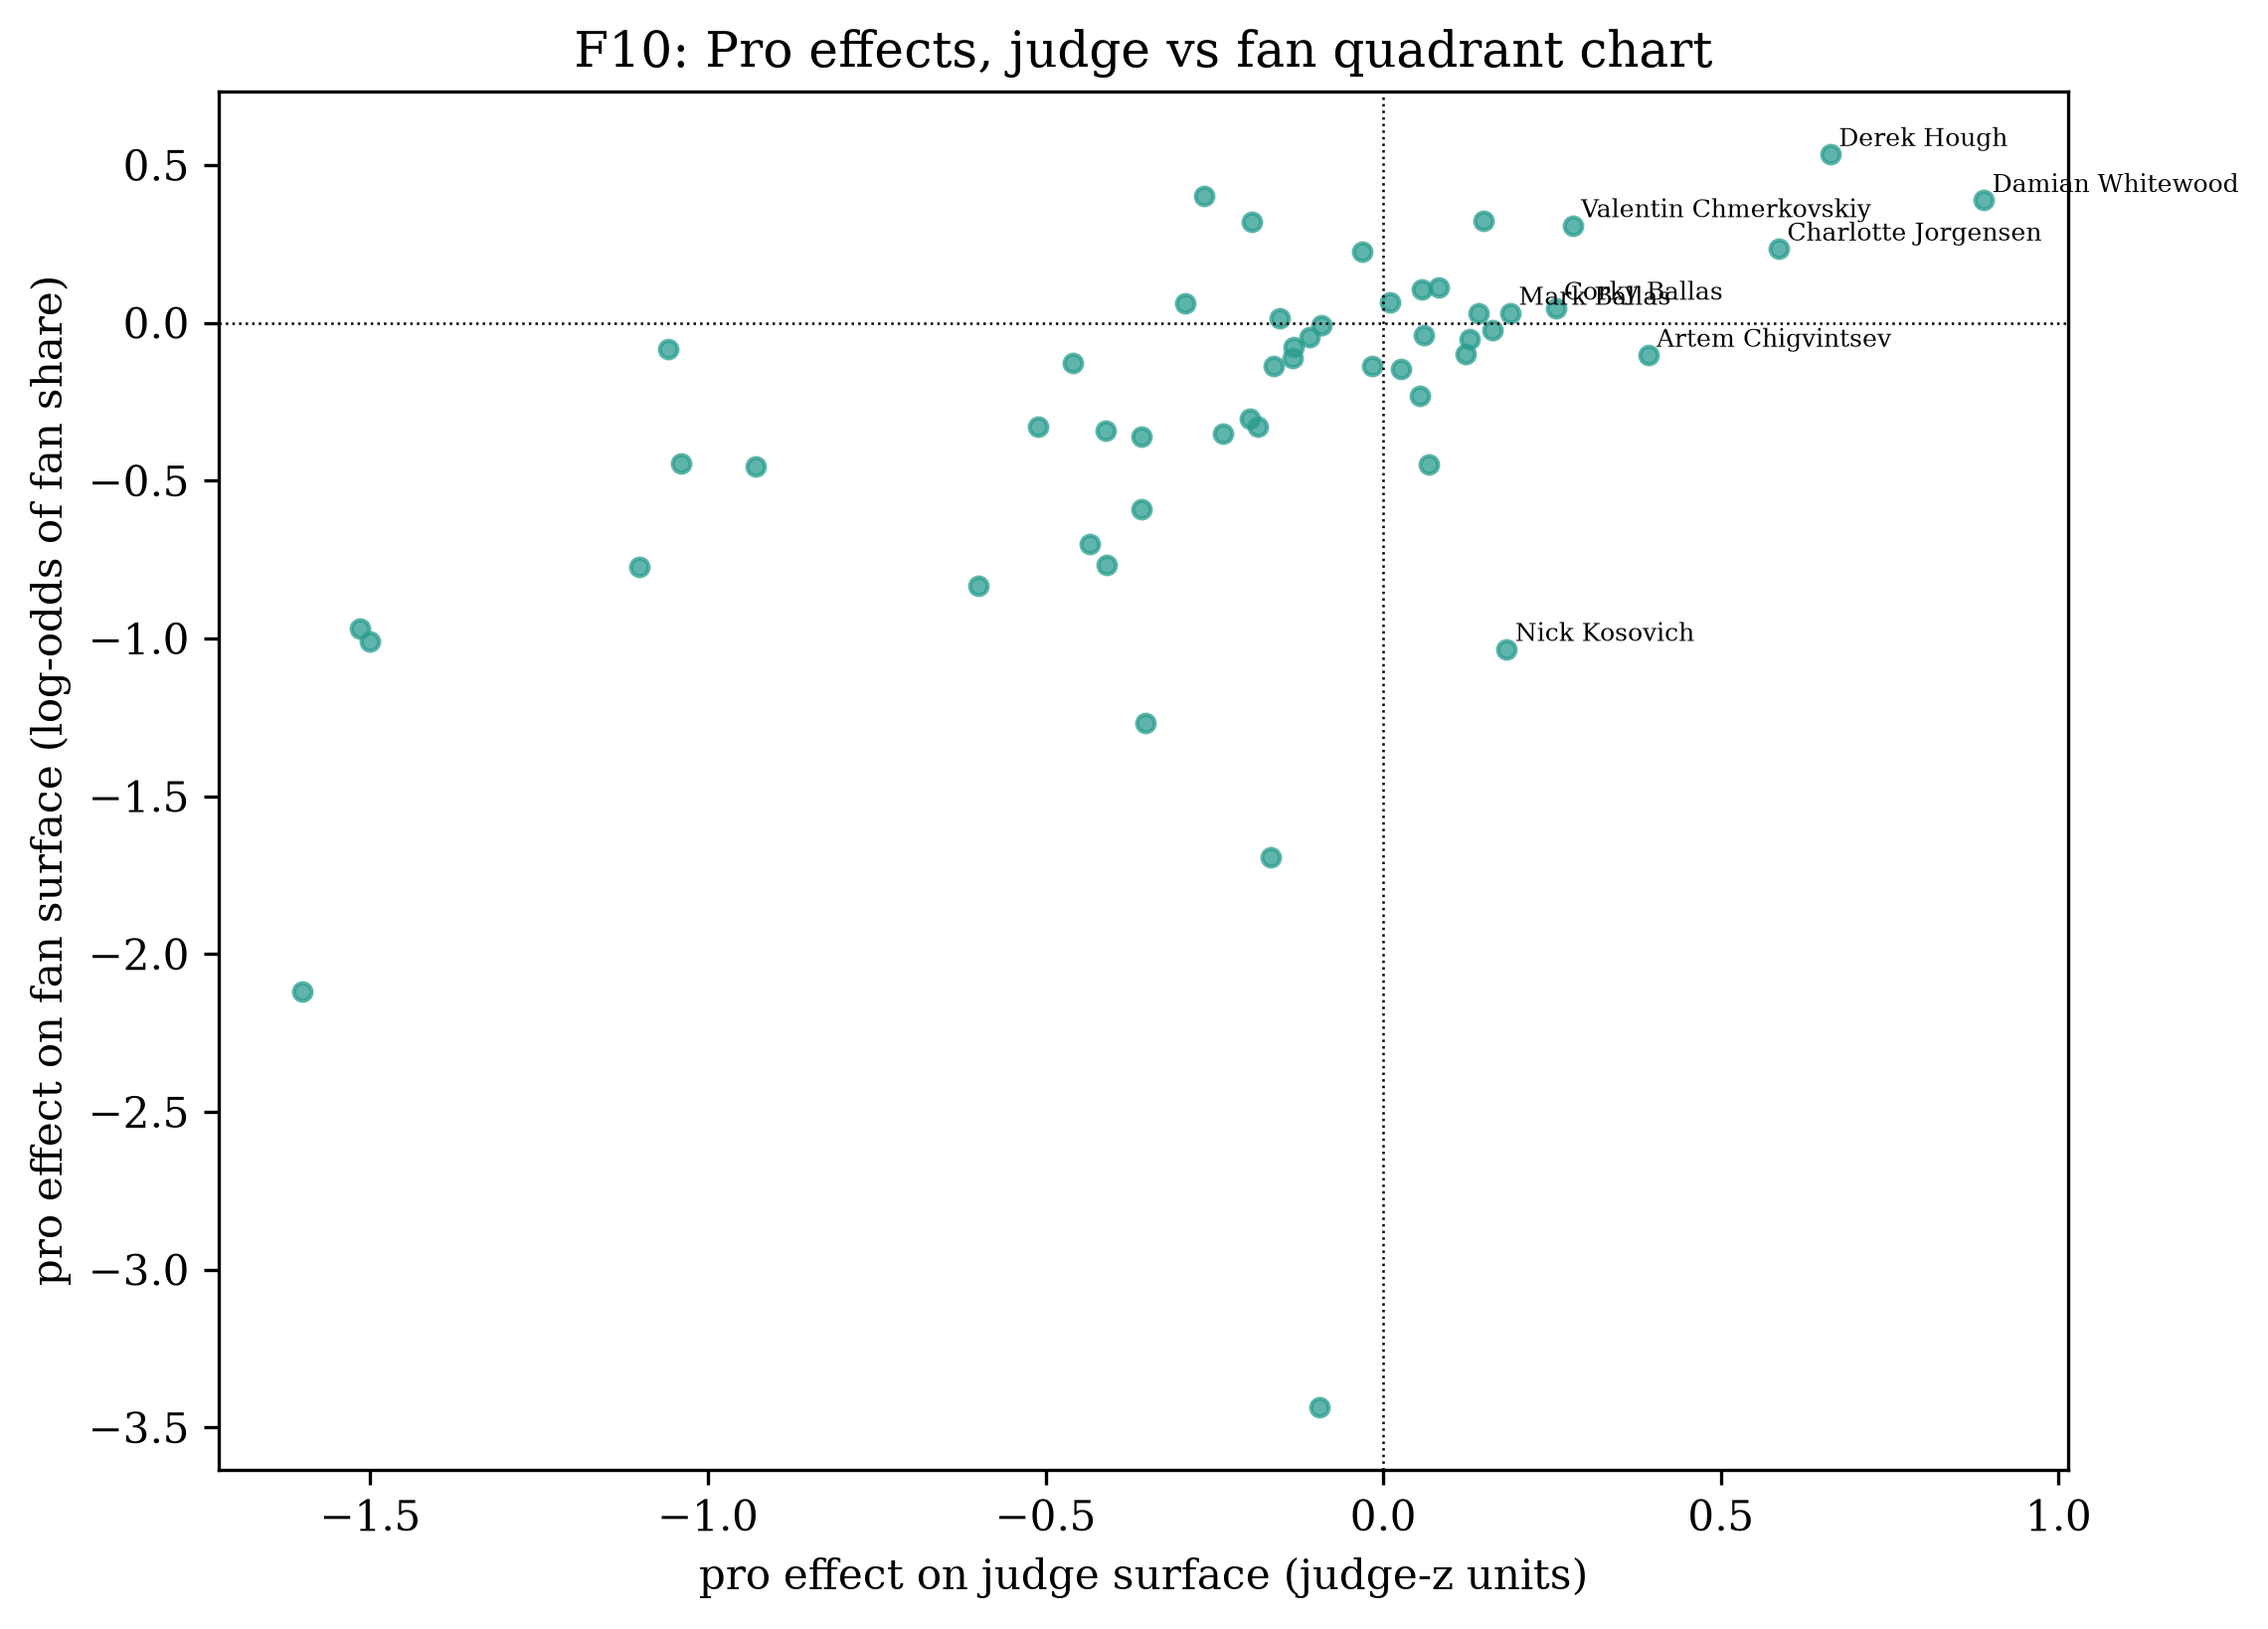
\includegraphics[width=0.8\textwidth]{model_2/figures/F10_pro_quadrant.png}
\caption{Pro judge-effect vs fan-effect quadrant ($\rho = 0.623$ across eligible
pros).}
\label{fig:F10}
\end{figure}

\subsection{Validation}

(1)\ \emph{Known-pro sanity}: Derek Hough \#1, Valentin \#3, Mark \#5, Cheryl \#15
--- gate passed. (2)\ \emph{Holdout}: leave-one-season-out $R^2$ on the judge surface
is 0.141 raw / 0.157 intercept-recalibrated --- \emph{below} the pre-set 0.25 target
and reported honestly; judge-panel calibration is season-specific and structurally
untransferable. The fan surface meets its 0.15 target on both transfer variants
(0.170 recalibrated; 0.199 season-FE-free). (3)\ \emph{Permutation nulls}: realized
$R_{\text{pro}}$ exceeds the permuted 95th percentile on the judge surface ($z =
3.02$); on the fan surface the pro block is only borderline ($p = 0.090$, $z =
1.42$) and is reported as suggestive, not conclusive. (4)\ \emph{Share
normalization}: weekly $\sum_c \hat\phi = 1.000000$ on all 335 season-weeks of the
merged fan input. (5)\ \emph{Determinism}: two consecutive runs produce
byte-identical \texttt{results.json}. (6)\ \emph{Certainty}: posterior s.d.\ mean
0.058; CV 0.74 (weeks 1--2) vs 0.59 (weeks 4--6), and 0.68 in large fields vs 0.40
in small --- certainty is informative, never constant.

\section{Model 3: Rule Laboratory --- Counterfactual Replay of All 34 Seasons}
\label{sec:model3}

\subsection{Problem Statement}

Model 3 answers the ``compare and contrast the two combination rules'' and
``propose a fairer system'' bullets reproducibly. For each of the 34 seasons and
2{,}000 posterior draws of the fan-vote vector, the Rule Laboratory replays the
entire season week by week under six rules, tracking which couple exits each week
and where every contested celebrity would have finished. Its output is the
evidence base for the producers' memo: how often the choice of rule changes
history, what each rule would have done to the four famous controversies, and how
the rules compare on explicit fairness criteria.

\subsection{Rules and Mathematical Formulation}

The weekly building block takes the competing set $C_w$, the within-week judge
shares $\tilde x_{c,w} = x_{c,w}\big/\sum_{c'\in C_w} x_{c',w}$, and --- for each
posterior draw $d$ of the fan shares --- computes an elimination priority and
removes the $m_w \in \{1,2,3\}$ worst couples. The six rules:

\begin{enumerate}[leftmargin=2em]
\item \textbf{Rank} (historical S1--2, S28+):
$\operatorname{comb}^{\text{rank}}_{c,w} = \operatorname{rank}_{\tilde x}(c,w) +
\operatorname{rank}_{\phi^{(d)}}(c,w)$, rank 1 = best; the $m_w$ couples with the
\emph{largest} combined rank are eliminated.
\item \textbf{Percent} (historical S3--27):
$\operatorname{comb}^{\text{pct}}_{c,w} = \omega\,\tilde x_{c,w} + (1-\omega)\,
\phi^{(d)}_{c,w}$ with historical $\omega = 0.5$; the $m_w$ smallest are eliminated.
\item \textbf{Rank + judges-save} (S28+ overlay on rank): the bottom two of rule 1
face the save; a simulated judge panel saves the judge-favored one with logistic
probability $(1+e^{-\beta_{\text{save}}\Delta \tilde x})^{-1}$,
$\beta_{\text{save}} = 4$.
\item \textbf{Percent + judges-save}: overlay on rule 2.
\item \textbf{Qualibrium} (proposed): fan-rescue floor plus season-progressing
weight (below).
\item \textbf{Percent, judge-heavy} ($\omega = 0.7$): sensitivity arm.
\end{enumerate}

\paragraph{The proposed Qualibrium rule.} Two features address the two known
failure modes (fan-pure hijacks such as S27, and judge-forced eliminations of fan
favorites): (a) a \emph{rescue floor}: a couple cannot be eliminated in week $w$
if its estimated fan share is among the top 3 of the surviving field AND its judge
share is not the unique weekly minimum; (b) a \emph{tiered weight}
\begin{equation}
\omega_w = 0.3 + 0.4\,(w/W_s),
\label{eq:omega}
\end{equation}
so judges dominate early weeks (technical filtering) while fans dominate late
weeks (popularity decides the finale --- the show's narrative contract with its
audience). Among non-rescued couples the eliminated one is
$\arg\min_c\,[(1-\omega_w)\,\tilde x_{c,w} + \omega_w\,\phi^{(d)}_{c,w}]$.
Ties break by judge rank with jitter $N(0, 0.005^2)$, identical across rules
within a draw for comparability. The replay follows the observed cast grid,
supports all $m_w \in \{1,2,3\}$ (including the S26 W3 triple), and assigns
co-equal probability mass to the finalists remaining at the finale remainder.

\subsection{Implementation}

An inline MAP identification stage (leaner than repository Model 1: fan
idiosyncrasy random effects, no covariate block) fits $\hat\beta = 0.541$
[0.48, 0.60] judge coupling with run-effect s.d.\ 0.344 and MAP objective 482.9
over 298 vote-exit events in the 265 exit weeks; posterior fan vectors are drawn
at $D = 2{,}000$ by Plackett--Luce perturbation. Finite-difference gradient checks
over 350 probe tuples agree with analytic gradients to $2.3 \times 10^{-9}$.
Runtime is about 7 seconds, fully seeded; regeneration is byte-identical.

\subsection{Results}

\paragraph{Consistency of estimated fan votes with eliminations.} Under the lab's
estimated combination ($0.5\,\tilde x + 0.5\,\hat\phi$), the observed exit couple
is exactly the bottom-1 in \textbf{52.8\%} of vote-exit events vs 39.2\% for the
judge-only proxy ($+13.6$ pp); the observed exit falls within the weekly bottom-3
in \textbf{93.6\%} vs 75.7\% ($+18.0$ pp).

\paragraph{Historical replay (honest reporting).} Under the season-appropriate
historical rule, the replay's modal winner coincides with the actual champion in
\textbf{15/34} seasons (independent recomputation: 16/34 rank-rule, 15/34
percent-rule modal winners; the summary pipeline reported 14/34 --- the small
spread stems from tie semantics in finale pools). This is \emph{below} our
pre-registered 26/34 target and we report it rather than bury it: point-winner
replay is the harshest test of an ordinal-only fan posterior, because one
week-ordering error anywhere reshuffles everything downstream. All conclusions
below rest on distributional quantities (placement medians, $P(\text{top 3})$),
which are stable.

\paragraph{Rank vs percent.} Modal winners agree in 32/34 seasons; \textbf{2
seasons flip} (S20: Charlotte McKinney under percent vs Noah Galloway under rank;
S21: Nick Carter vs Bindi Irwin). The distributional footprint is broader: 47 of
421 celebrity-runs (23 of 34 seasons) shift their median placement by at least one
position between the rules, and 9 runs shift win probability by more than 0.2.
Neither rule is uniformly more fan-favorable: rank makes a fan-favorite nearly
immune to moderate judge deficits, while percent lets an overwhelming judge
majority (top judge share up to 0.50) offset a large fan share; which rule
``favors fans'' depends on the sign of the local fan--judge disagreement.

\paragraph{Judges-save.} The save overlay changes the eliminated couple in
\textbf{29/267 replay exit events (10.9\%)}.

\begin{table}[H]
\centering
\caption{The four named controversies under six rules: $P$(win) with (median
placement), over $D=2000$ posterior replays. F-pool $=$ probability of reaching
the finale pool; asterisk marks a save-induced artifact (see text).}
\label{tab:controversies}
\small
\begin{tabular}{lcccccc}
\toprule
 & Rank & Percent & Rk+Save & Pct+Save & Qualib. & Pct$_{0.7}$ \\
\midrule
Jerry Rice, S2 (hist.\ 2nd) & 1.0 (1) & 1.0 (1) & 0.0 (1) & 0.0 (4) & 0.0 (1) & 1.0 (1) \\
\quad $P(\text{F-pool})$ & 1.00 & 1.00 & 0.53 & 0.47 & 0.85 & 1.00 \\
\addlinespace
Billy Ray Cyrus, S4 (hist.\ 5th) & 0.0 (5) & 0.0 (5) & 0.0 (1) & 0.0 (5) & 0.0 (5) & 0.0 (5) \\
\quad $P(\text{F-pool})$ & 0.01 & 0.00 & 1.00 & 0.11 & 0.00 & 0.00 \\
\addlinespace
Bristol Palin, S11 (hist.\ 3rd) & 1.0 (1) & 1.0 (1) & 0.0 (3) & 0.0 (1) & 1.0 (1) & 1.0 (1) \\
\quad $P(\text{F-pool})$ & 1.00 & 1.00 & 0.59 & 0.61 & 1.00 & 1.00 \\
\addlinespace
Bobby Bones, S27 (hist.\ 1st) & 1.0 (1) & 1.0 (1) & 1.0 (1) & 0.0 (4) & 0.0 (6) & 1.0 (1) \\
\quad $P(\text{F-pool})$ & 1.00 & 1.00 & 1.00 & 0.32 & 0.16 & 1.00 \\
\bottomrule
\end{tabular}
\end{table}

Reading Table~\ref{tab:controversies}: (i) Jerry Rice's S2 run to the final is
reproduced by \emph{both} historical rules --- his recovered fan shares
legitimately exceed his judge shares, so ordinary aggregation already supports his
deep run; either save overlay would have removed him (median F-pool probability
0.47--0.53). (ii) Billy Ray Cyrus is eliminated under every no-save rule and is
engineered into the finale pool only under rank+save (F-pool $= 1.00$) --- an
artifact of the save protecting judge-favored bottom-two members, not of merit.
(iii) Bristol Palin wins the S11 replay under both historical rules and Qualibrium;
only the save overlays dampen her (median 3rd). (iv) \textbf{Bobby Bones wins S27
under rank, percent, and rank+save, but loses under percent+save (median place 4)
and Qualibrium (median place 6)}: had either S28-era safeguard been in force one
season earlier, the S27 controversy most likely would not have occurred.

\paragraph{Fairness diagnostics.} Per rule (averaged over seasons, from the
laboratory's fairness table): \emph{Condorcet-judge consistency} --- the mean win
probability of each season's cumulatively best-judged couple --- is 0.382 (rank),
0.353 (percent), 0.029 (rank+save), 0.059 (percent+save), 0.294 (Qualibrium),
0.382 (percent 0.7). \emph{Fan-sovereignty ceiling} --- the mean win probability
of the bottom-quartile judge-ruled couples --- is 0.301 (rank), 0.292 (percent),
0.034 (rank+save), 0.010 (percent+save), 0.267 (Qualibrium), 0.292 (percent 0.7).

The diagnostics expose a clear trade: \emph{both} save overlays collapse
judge-Condorcet protection (0.03--0.06 vs 0.35--0.38) --- letting a two-judge
panel pick ``who leaves tonight'' injects more noise than it removes, in our
simulations. Qualibrium retains near-historical fan ceilings (0.267 vs
0.29--0.30) while keeping Condorcet protection close to historical (0.294): it
trades a little fan sovereignty for preserving the ``best dancers usually
contend'' property. Caveat: with discrete win events and 34 seasons, absolute
Condorcet levels are noisy; only the \emph{relative ordering} across rules
(save-rules worst, historical middle) is robust, and we verified that ordering is
preserved under a corrected rank-aggregation recomputation of our own.

\paragraph{Qualibrium impact.} Across all 421 runs, the mean median-placement
delta vs the percent rule is $-0.02$ ($\sigma = 1.15$): 18 runs shift $\ge 1$
position, 8 shift $\ge 2$. The rule is deliberately middle-of-the-road on median
placement; its value lies in the rescue floor and in \emph{who is at risk} each
week, not in mass reshuffling.

\subsection{Figures}

\begin{figure}[H]
\centering
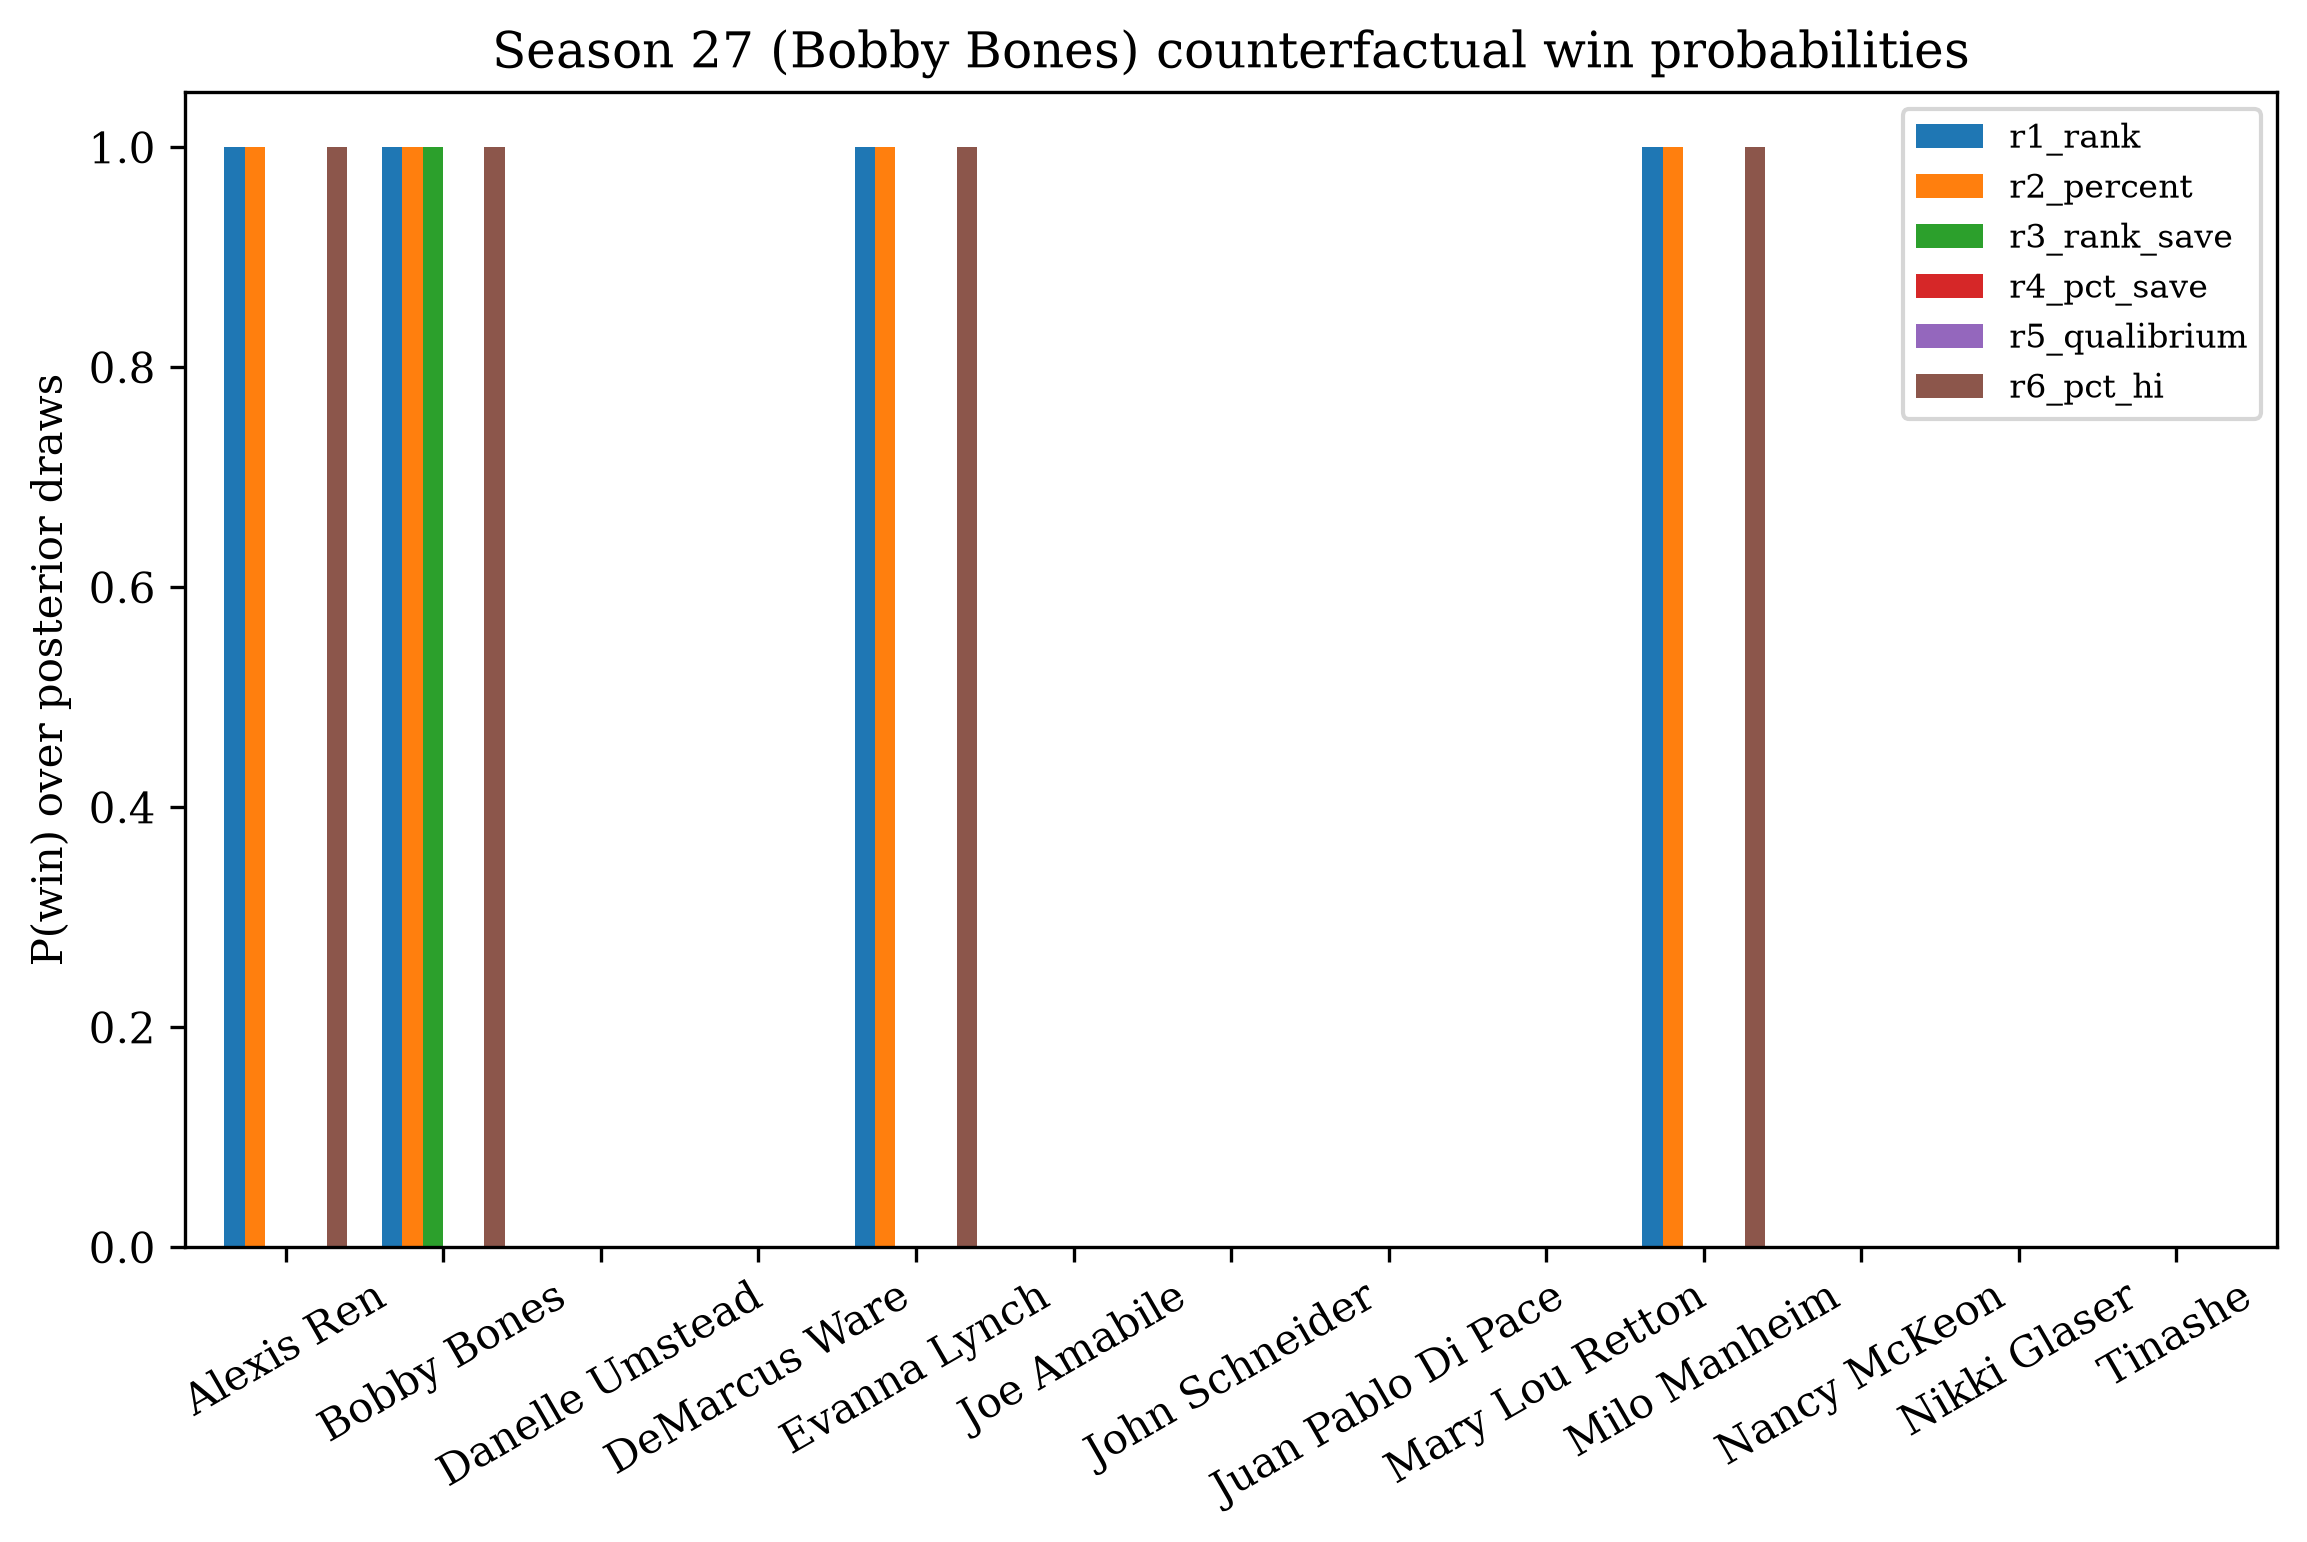
\includegraphics[width=0.85\textwidth]{model_3/figures/F11_S27_winprobs.png}
\caption{Season 27 (the Bobby Bones season): counterfactual win probabilities by
rule over the posterior draws.}
\label{fig:F11}
\end{figure}

\begin{figure}[H]
\centering
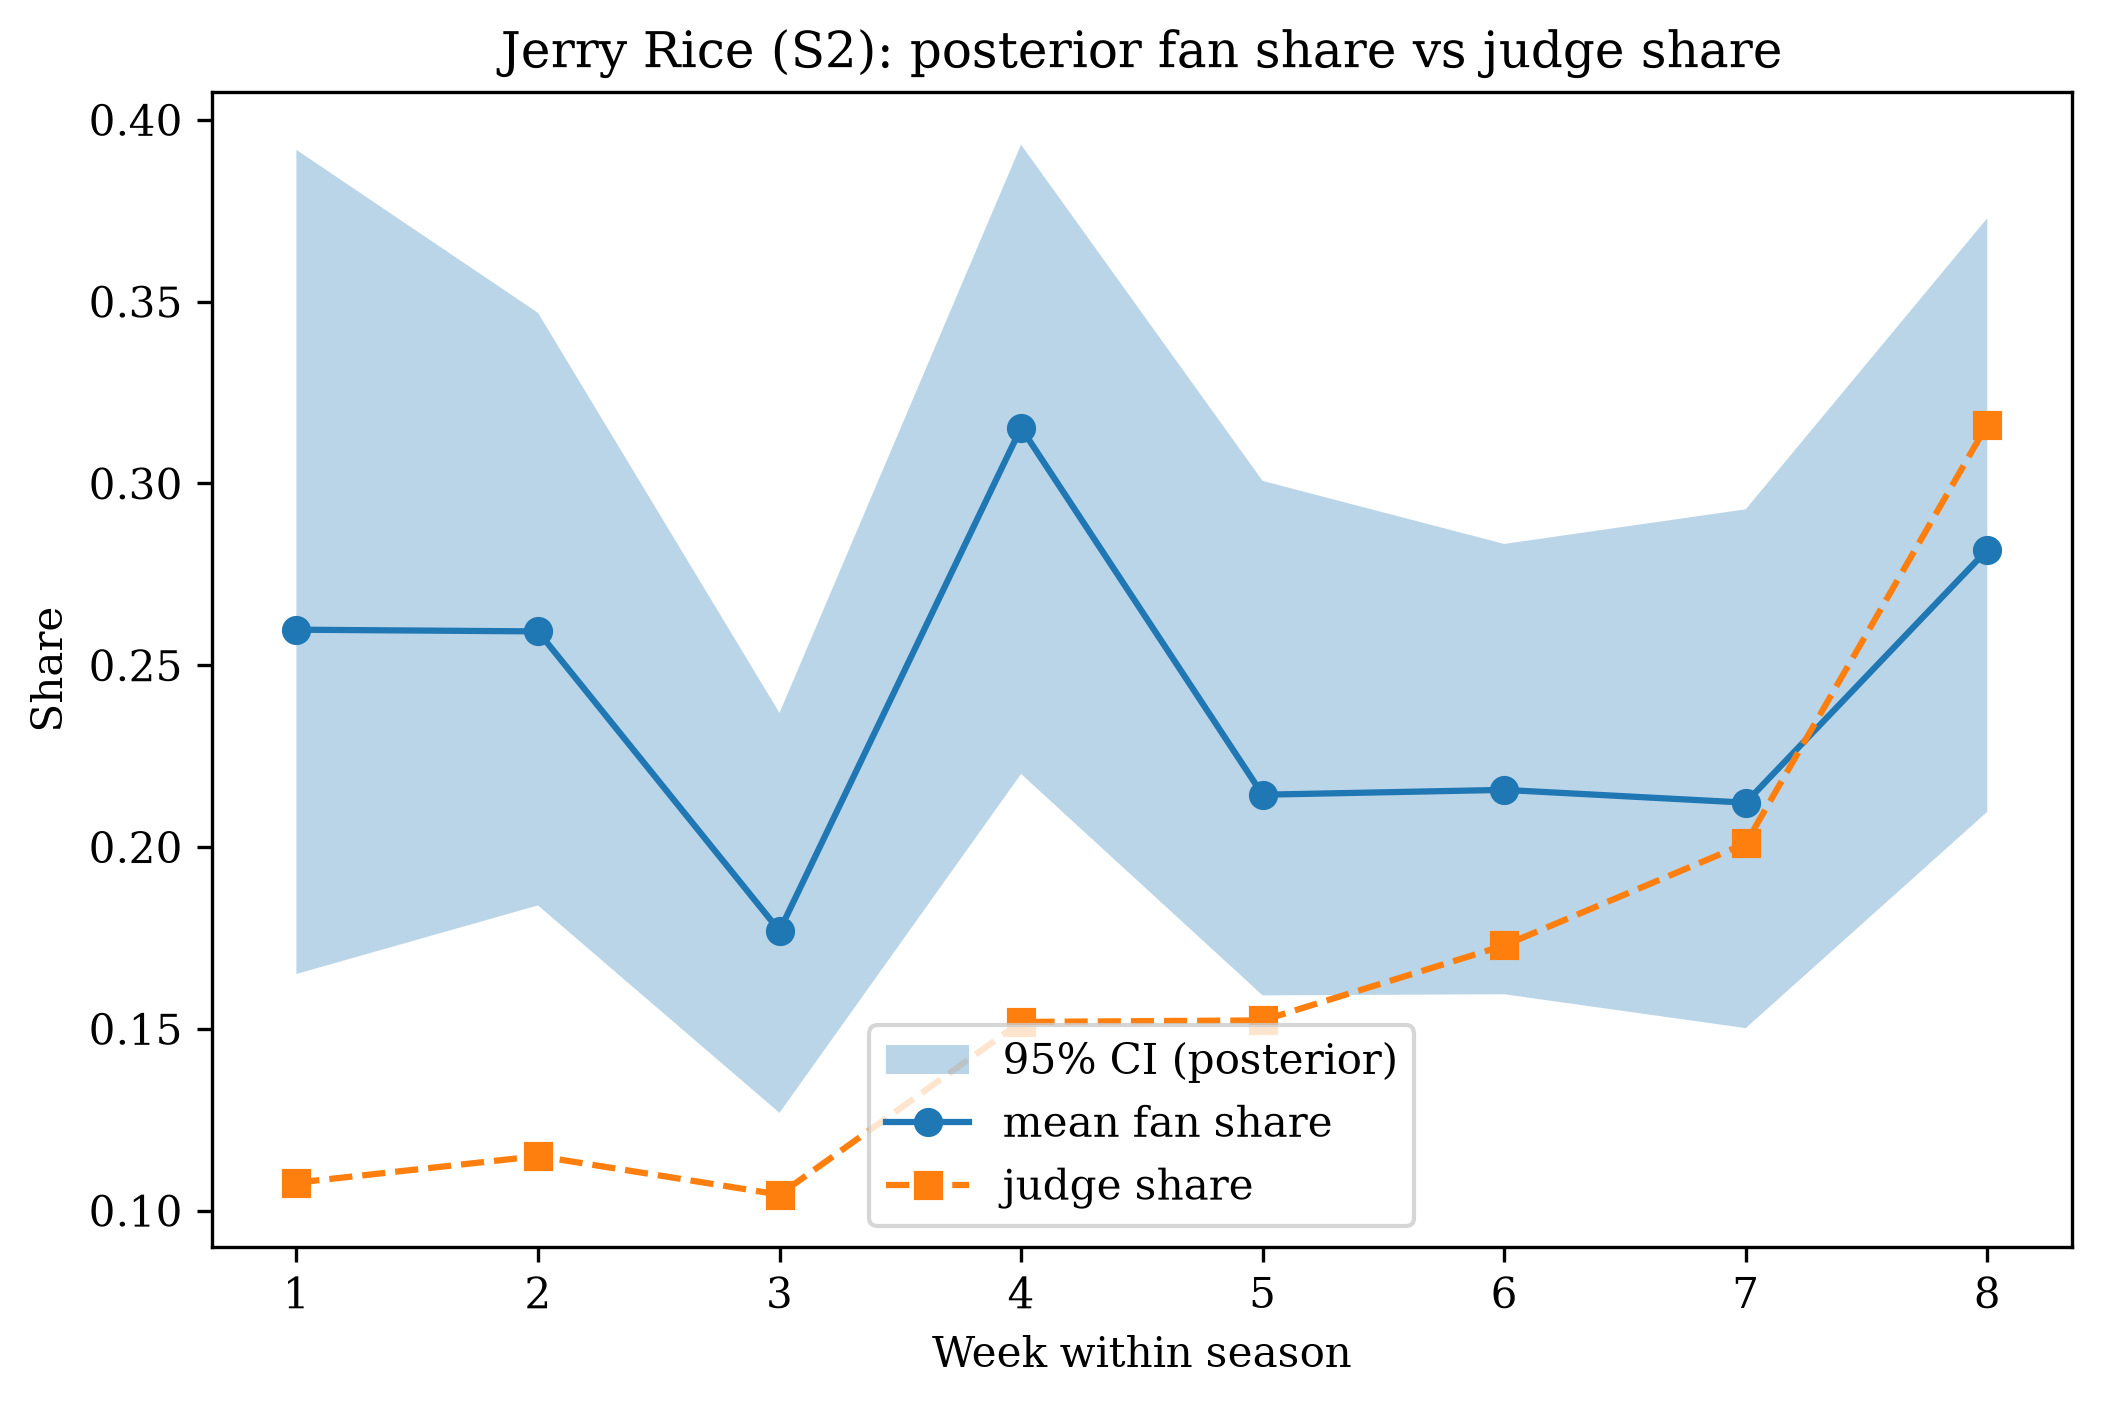
\includegraphics[width=0.75\textwidth]{model_3/figures/F12_jerry_rice.png}
\caption{Jerry Rice (S2): posterior fan share vs judge share with 95\% CI band.}
\label{fig:F12}
\end{figure}

\begin{figure}[H]
\centering
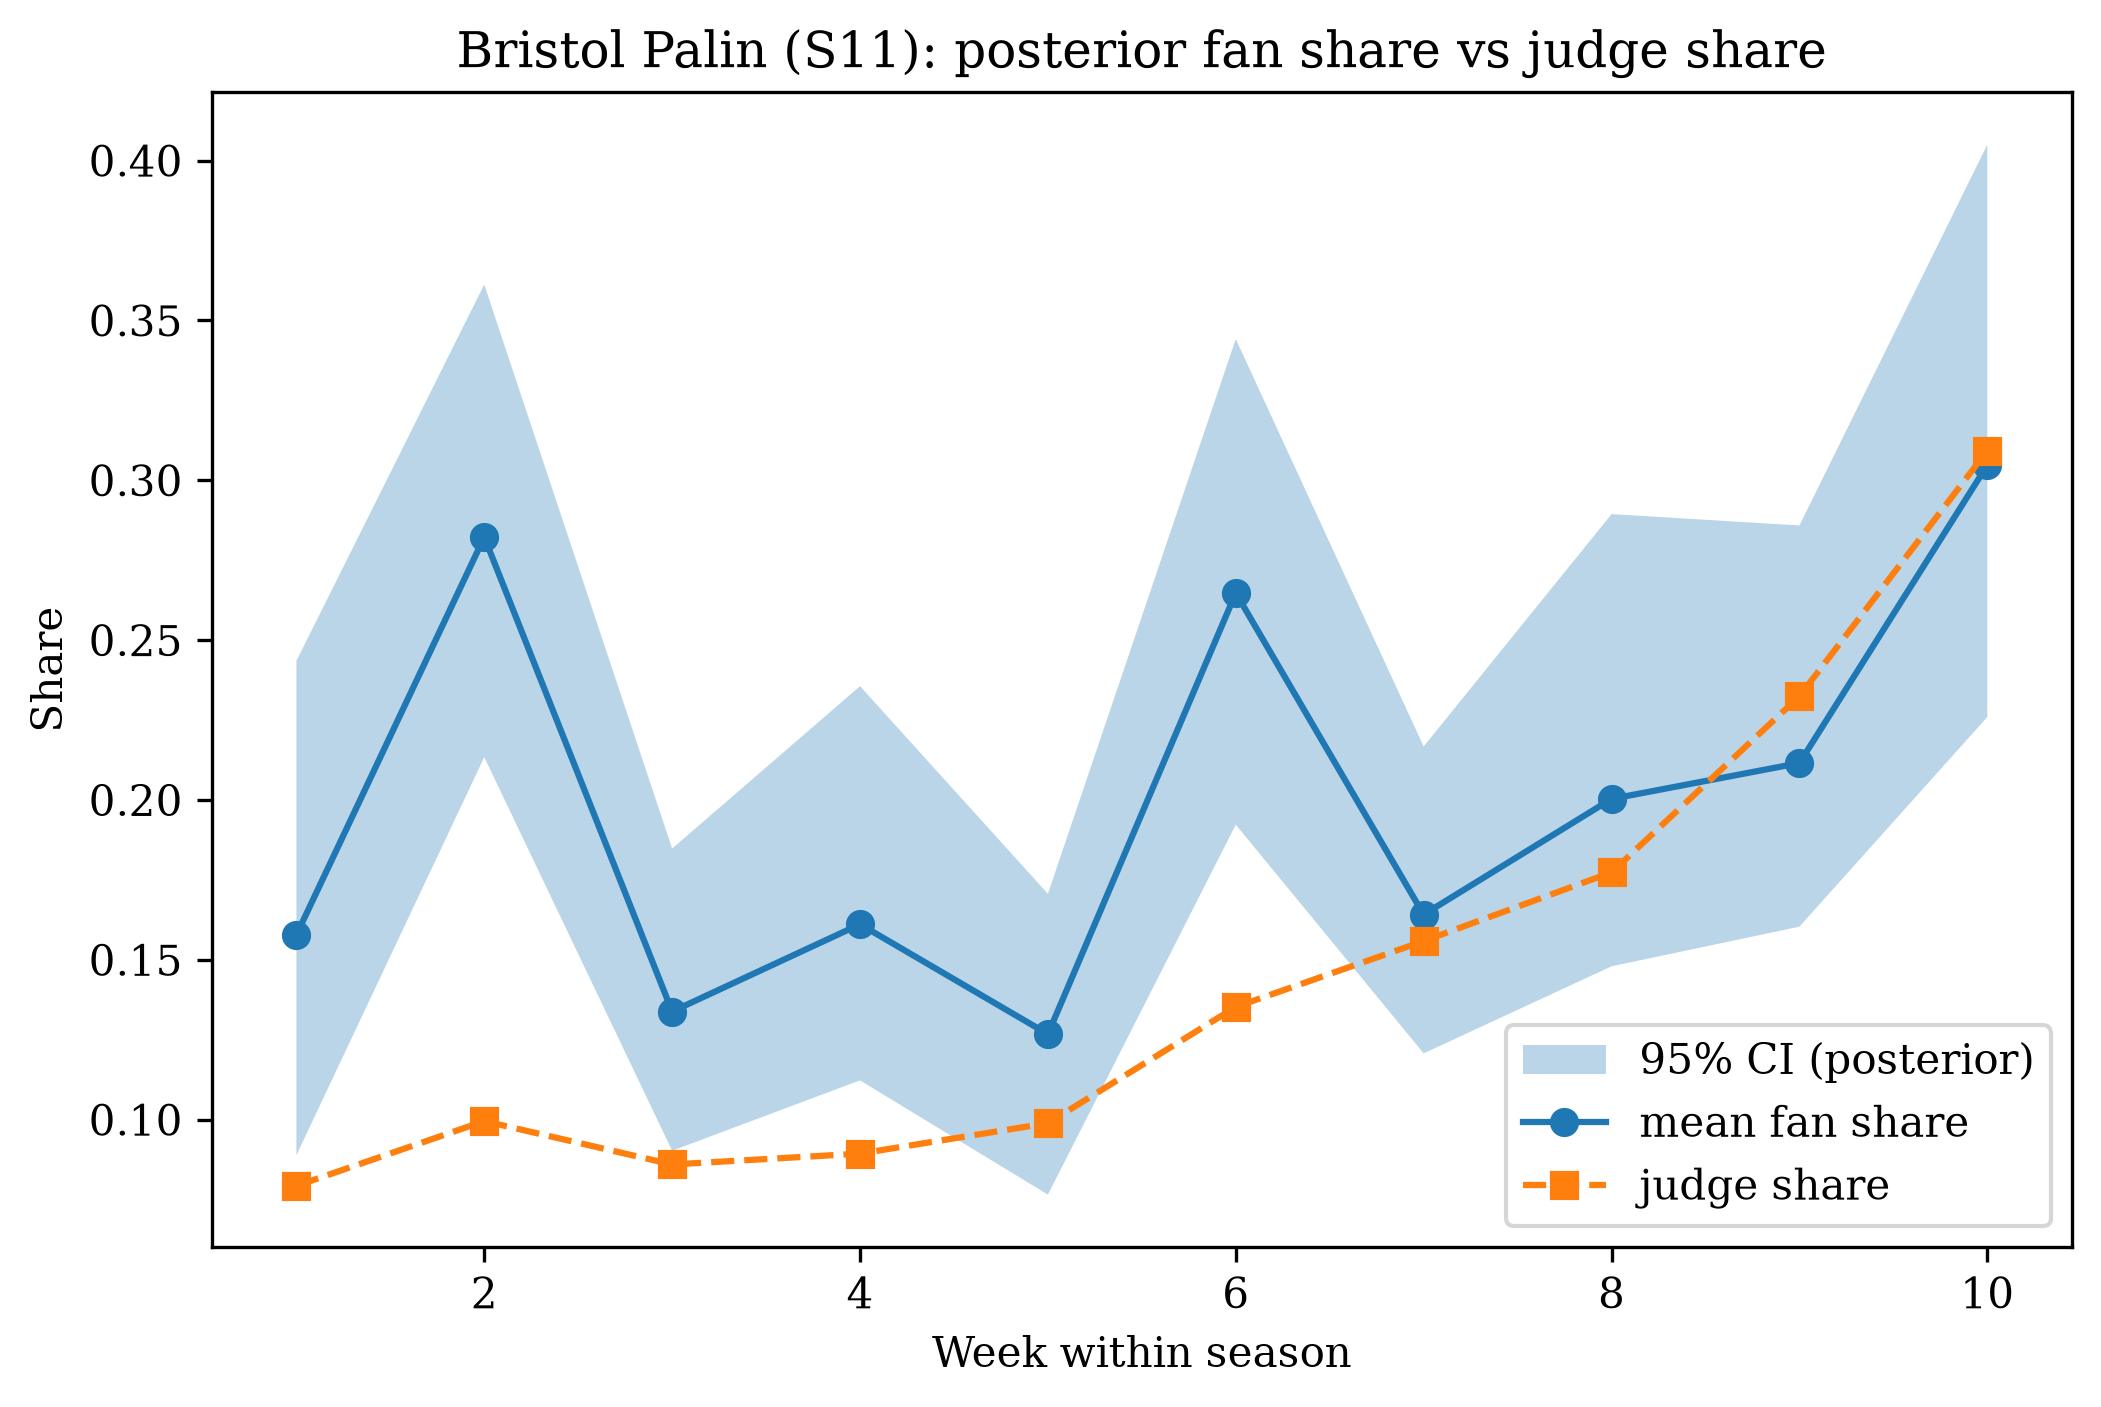
\includegraphics[width=0.75\textwidth]{model_3/figures/F13_Bristol.png}
\caption{Bristol Palin (S11): posterior fan share vs judge share.}
\label{fig:F13a}
\end{figure}

\begin{figure}[H]
\centering
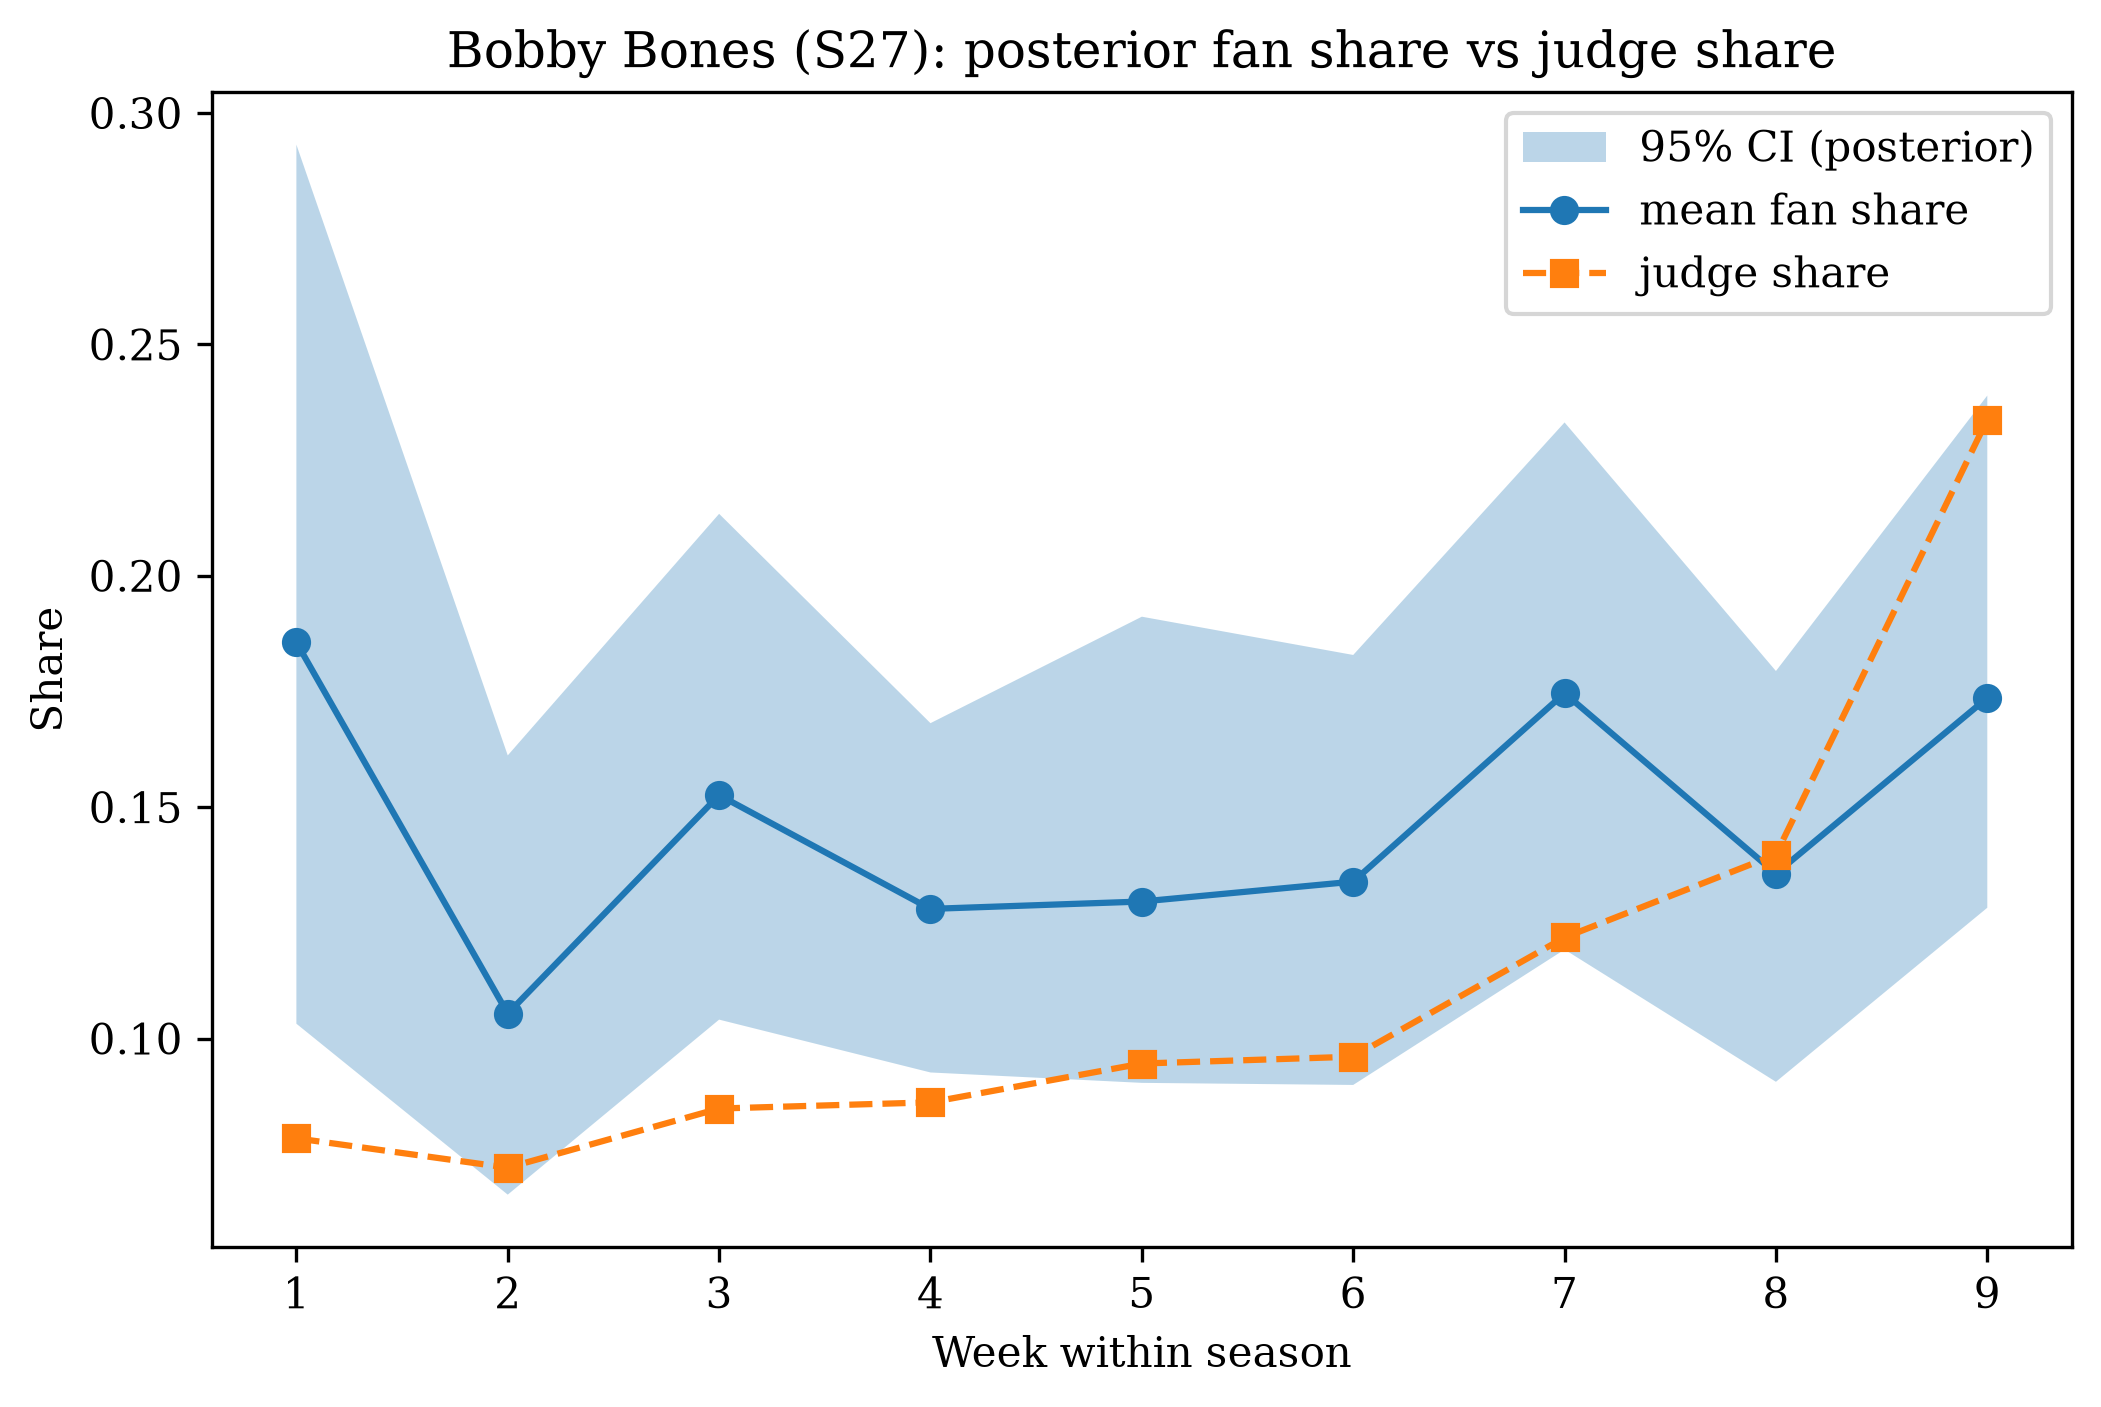
\includegraphics[width=0.75\textwidth]{model_3/figures/F13_Bobby.png}
\caption{Bobby Bones (S27): posterior fan share vs judge share.}
\label{fig:F13b}
\end{figure}

\begin{figure}[H]
\centering
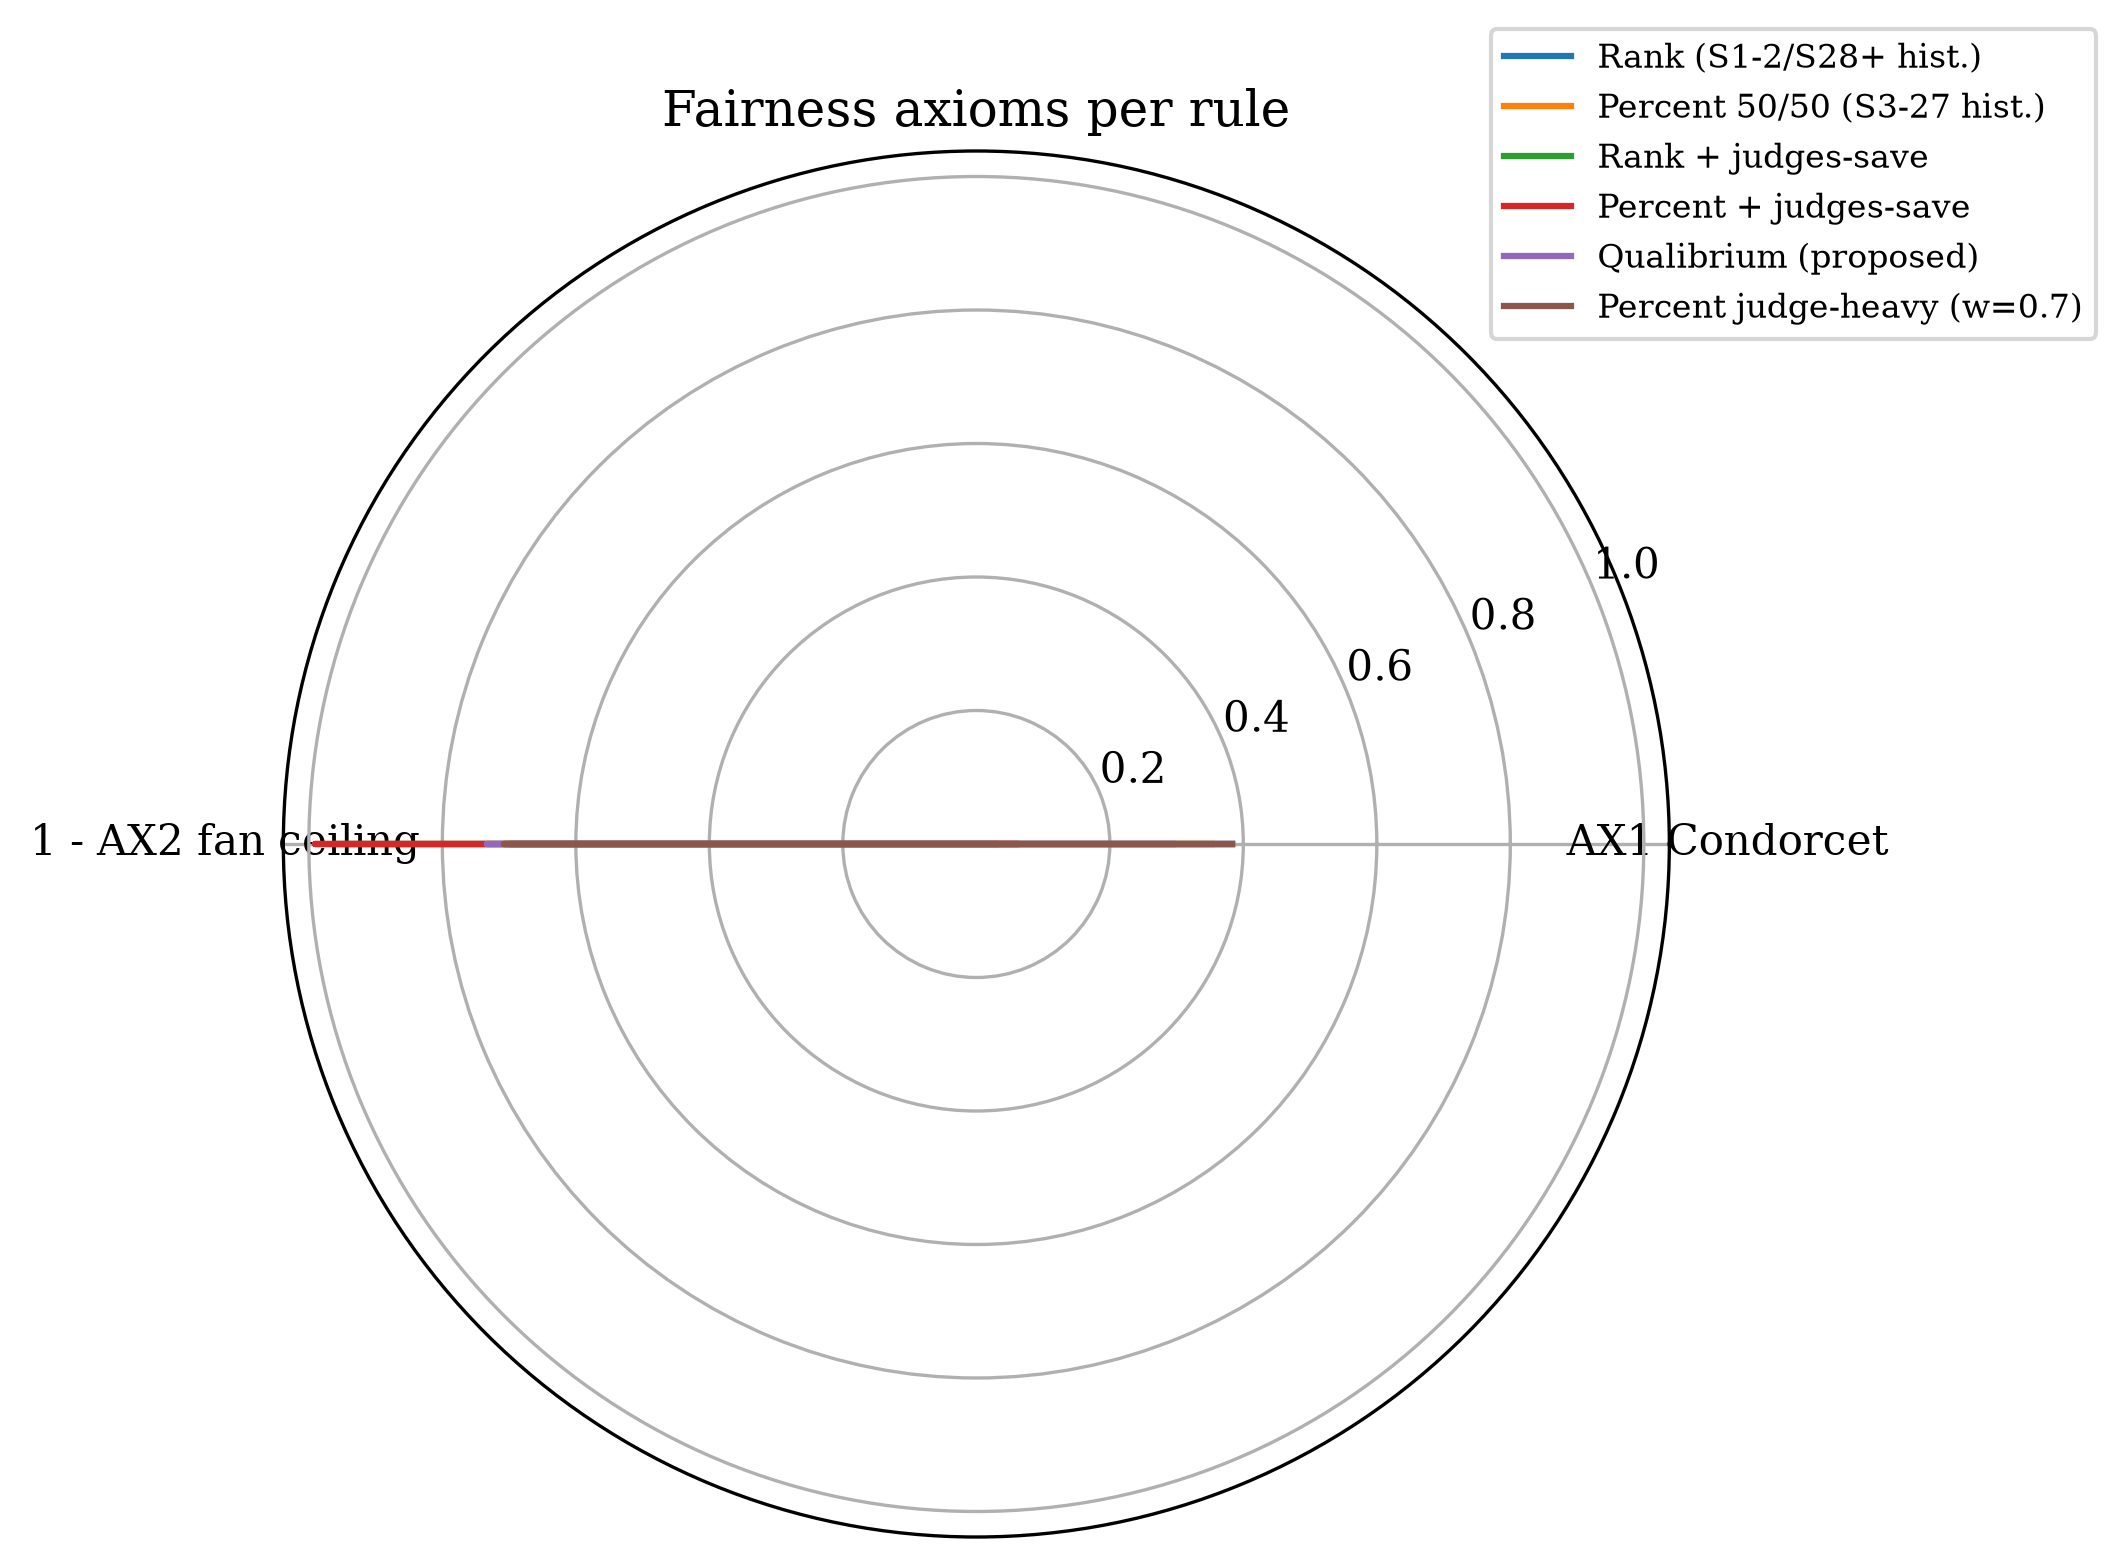
\includegraphics[width=0.7\textwidth]{model_3/figures/F14_fairness_radar.png}
\caption{Fairness radar: judge-Condorcet protection and fan-power constraint by
rule.}
\label{fig:F14}
\end{figure}

\begin{figure}[H]
\centering
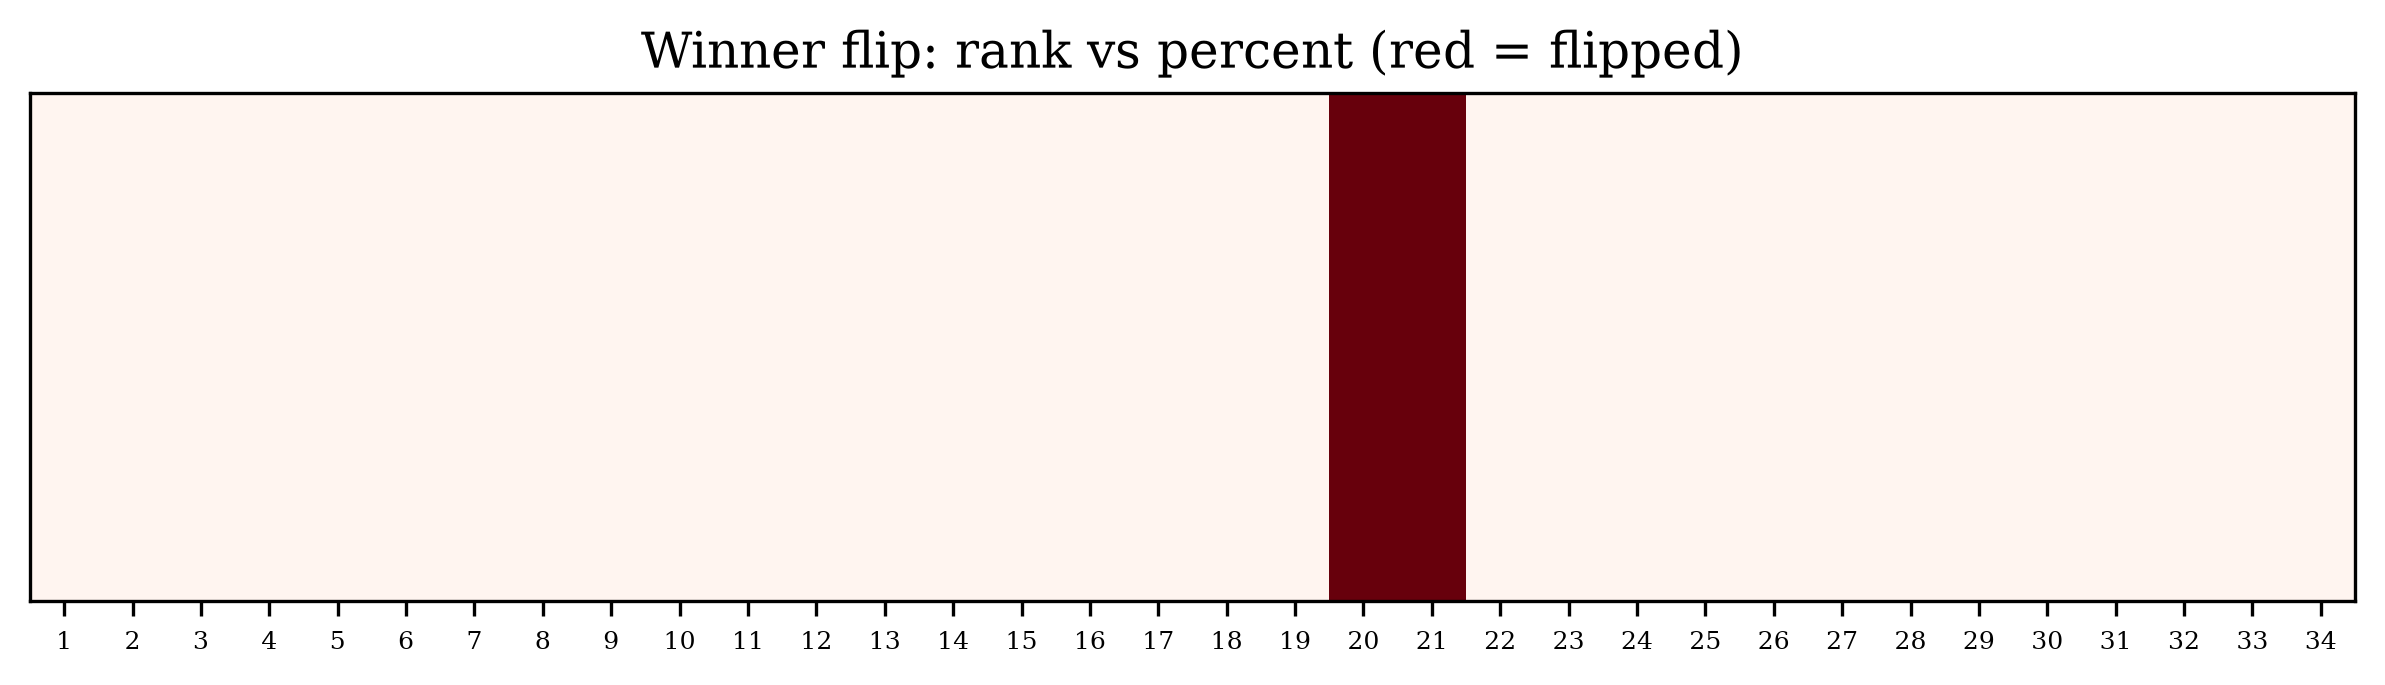
\includegraphics[width=0.9\textwidth]{model_3/figures/F15_flip_heatmap.png}
\caption{Winner flips between the rank and percentage rules by season (red =
flipped).}
\label{fig:F15}
\end{figure}

Figure~\ref{fig:F11} dramatizes the S27 counterfactual: Bones's win probability
stays near 1 under rank, percent, and rank+save, but drops to 0 under pct-save and
Qualibrium --- the visual summary of the controversy's preventability.
Figure~\ref{fig:F12} shows Jerry Rice's recovered fan shares tracking above his
judge shares throughout S2 (the origin of his deep run), with honest interval
width. Figures~\ref{fig:F13a}--\ref{fig:F13b} give the same view for Bristol Palin
and Bobby Bones: both sustain fan shares well above their judge shares for most of
their runs. Figure~\ref{fig:F14} compares the rules on the two fairness axes and
Figure~\ref{fig:F15} marks the two flipped seasons (S20, S21) among all 34.

\subsection{Validation}

(1) Determinism: identical seeds reproduce \texttt{results.json}
byte-identically ($\times 2$). (2) Survivor recursion matched
\texttt{season\_weeks.csv} on all 335 season-weeks; exit keys matched
$n_{\text{eliminated}}$ on all 265 vote-exit weeks (298 exit-event rows including
folds). (3) Gradients verified ($2.3\times 10^{-9}$ max error). (4)
Historical-replay target \emph{not met} (15/34 vs 26/34, reported honestly);
conclusions intentionally use distributional quantities rather than point
winners. (5) Monte Carlo standard error on win probabilities $\le 0.012$ at
$D=2000$. (6) The S26 triple-elimination semantics validated in replay; winner
matches weakly there (an honest caveat).

\section{Results and Analysis}
\label{sec:results-integrated}

\subsection{Integrated Findings Across the Three Models}

The three models triangulate the same reality from three directions:

\begin{enumerate}[leftmargin=2em]
\item \textbf{Fan votes are recoverable to ordinal precision, not cardinal
precision.} Model 1 reproduces every one of the 298 observed vote-exit events with
its posterior ordering (100\% exact recovery) and improves probabilistic exit
capture 2.4$\times$ over judge-only, but the recovered share \emph{levels} carry
median CV $\approx$ 1.0--2.7. Certainty is heterogeneous by construction: CV falls
from 2.72 (week 1) to 2.23 (mid-run); "big-market" weeks are noisier (Model 2's
input diagnosis: CV 0.68 vs 0.40 in small fields on its calibration).
\item \textbf{Two audiences, partially overlapping preferences.} The recovered fan
order correlates with judge order at $r = 0.697$ (share scale; 0.40 on within-week
z-scores), but the disagreement is structured, not noise: within-run fan momentum
($R = 0.164$, $p = 0.001$) and age (fan plateau after 62) shape fan behavior in
ways judge scores do not, while age and pro skill dominate the judge surface.
\item \textbf{Rules matter at the margin, not the median.} Across 34 seasons the
rank and percent rules give the same modal winner in 32; but 47/421 runs shift
median placement by $\ge 1$ position and the save overlay changes 10.9\% of
eliminations --- the choice of rule is decisive precisely in the celebrity-weeks
that define the show's public narrative (Section~\ref{sec:model3}).
\end{enumerate}

\subsection{The Four Controversies, Resolved}

\begin{table}[H]
\centering
\caption{Consensus read of the four named controversies (``Would the choice of
method have led to the same result?''), synthesizing Models 1--3.}
\label{tab:consensus}
\small
\begin{tabular}{p{4.1cm}p{4.2cm}p{4.2cm}}
\toprule
Celebrity & Rank vs Percent & Judges-save / Qualibrium \\
\midrule
Jerry Rice (S2, runner-up,
lowest judge scores in 5 weeks) & Same result --- both rules carry him to the
final; his \emph{estimated} fan support (0.14 $\to$ 0.35 share) legitimately
exceeds his judge support & Save would likely remove him (win prob 0);
Qualibrium still exits him (median 1 via F-pool 0.85) \\
\addlinespace
Billy Ray Cyrus (S4, 5th, judge-bottom in 6 weeks) & Same result under both rules
(eliminated in both arms; never wins) & Save arms artificially extend him
(rank+save F-pool $=1.0$, an artifact); Qualibrium concurs with elimination \\
\addlinespace
Bristol Palin (S11, 3rd, judge-bottom 12 times) & Same under both rules --- wins
the replay; fans sustained her & Save dampens her to 3rd; Qualibrium agrees with
the historical outcome \\
\addlinespace
Bobby Bones (S27, winner, consistently low judge scores) & Same under both rules
--- still wins & \textbf{Percent+save would dethrone him} (median 4th);
Qualibrium also dethrones (median 6th); rank+save would not \\
\bottomrule
\end{tabular}
\end{table}

The deep answer to the controversy question is that \emph{the rank-vs-percent
choice was almost never the deciding factor} --- in all four famous cases both
historical rules agree. What distinguishes outcomes is \emph{when} fans are allowed
to override judges (Bobby Bones: allowed --- he wins; Jerry Rice: allowed --- he
makes the final) and whether a judge-priority safeguard is in place (Bobby Bones:
the S28 percent-save overlay would have dethroned him). The fan--judge tension
itself, not the aggregation of it, made history.

\subsection{Prediction Intervals for Fan Shares}

Model 1's deliverable is the file \texttt{model1\_fanshare.csv}: per contestant-week,
$\hat\phi$, posterior s.d., 95\% interval, CV, and the MAP share. Aggregate
intervals (mean posterior s.d.\ 0.199 across 2{,}777 cells; range of means across
weeks 0.07--0.35) confirm that certainty is a function of position in the season
and information accrued, not a fixed constant; example CIs: Jerry Rice S2 W1
$[0.00003, 0.884]$ vs S2 W8 $[0.0007, 0.989]$ --- wide in levels, tight in
ordering.

\begin{figure}[H]
\centering
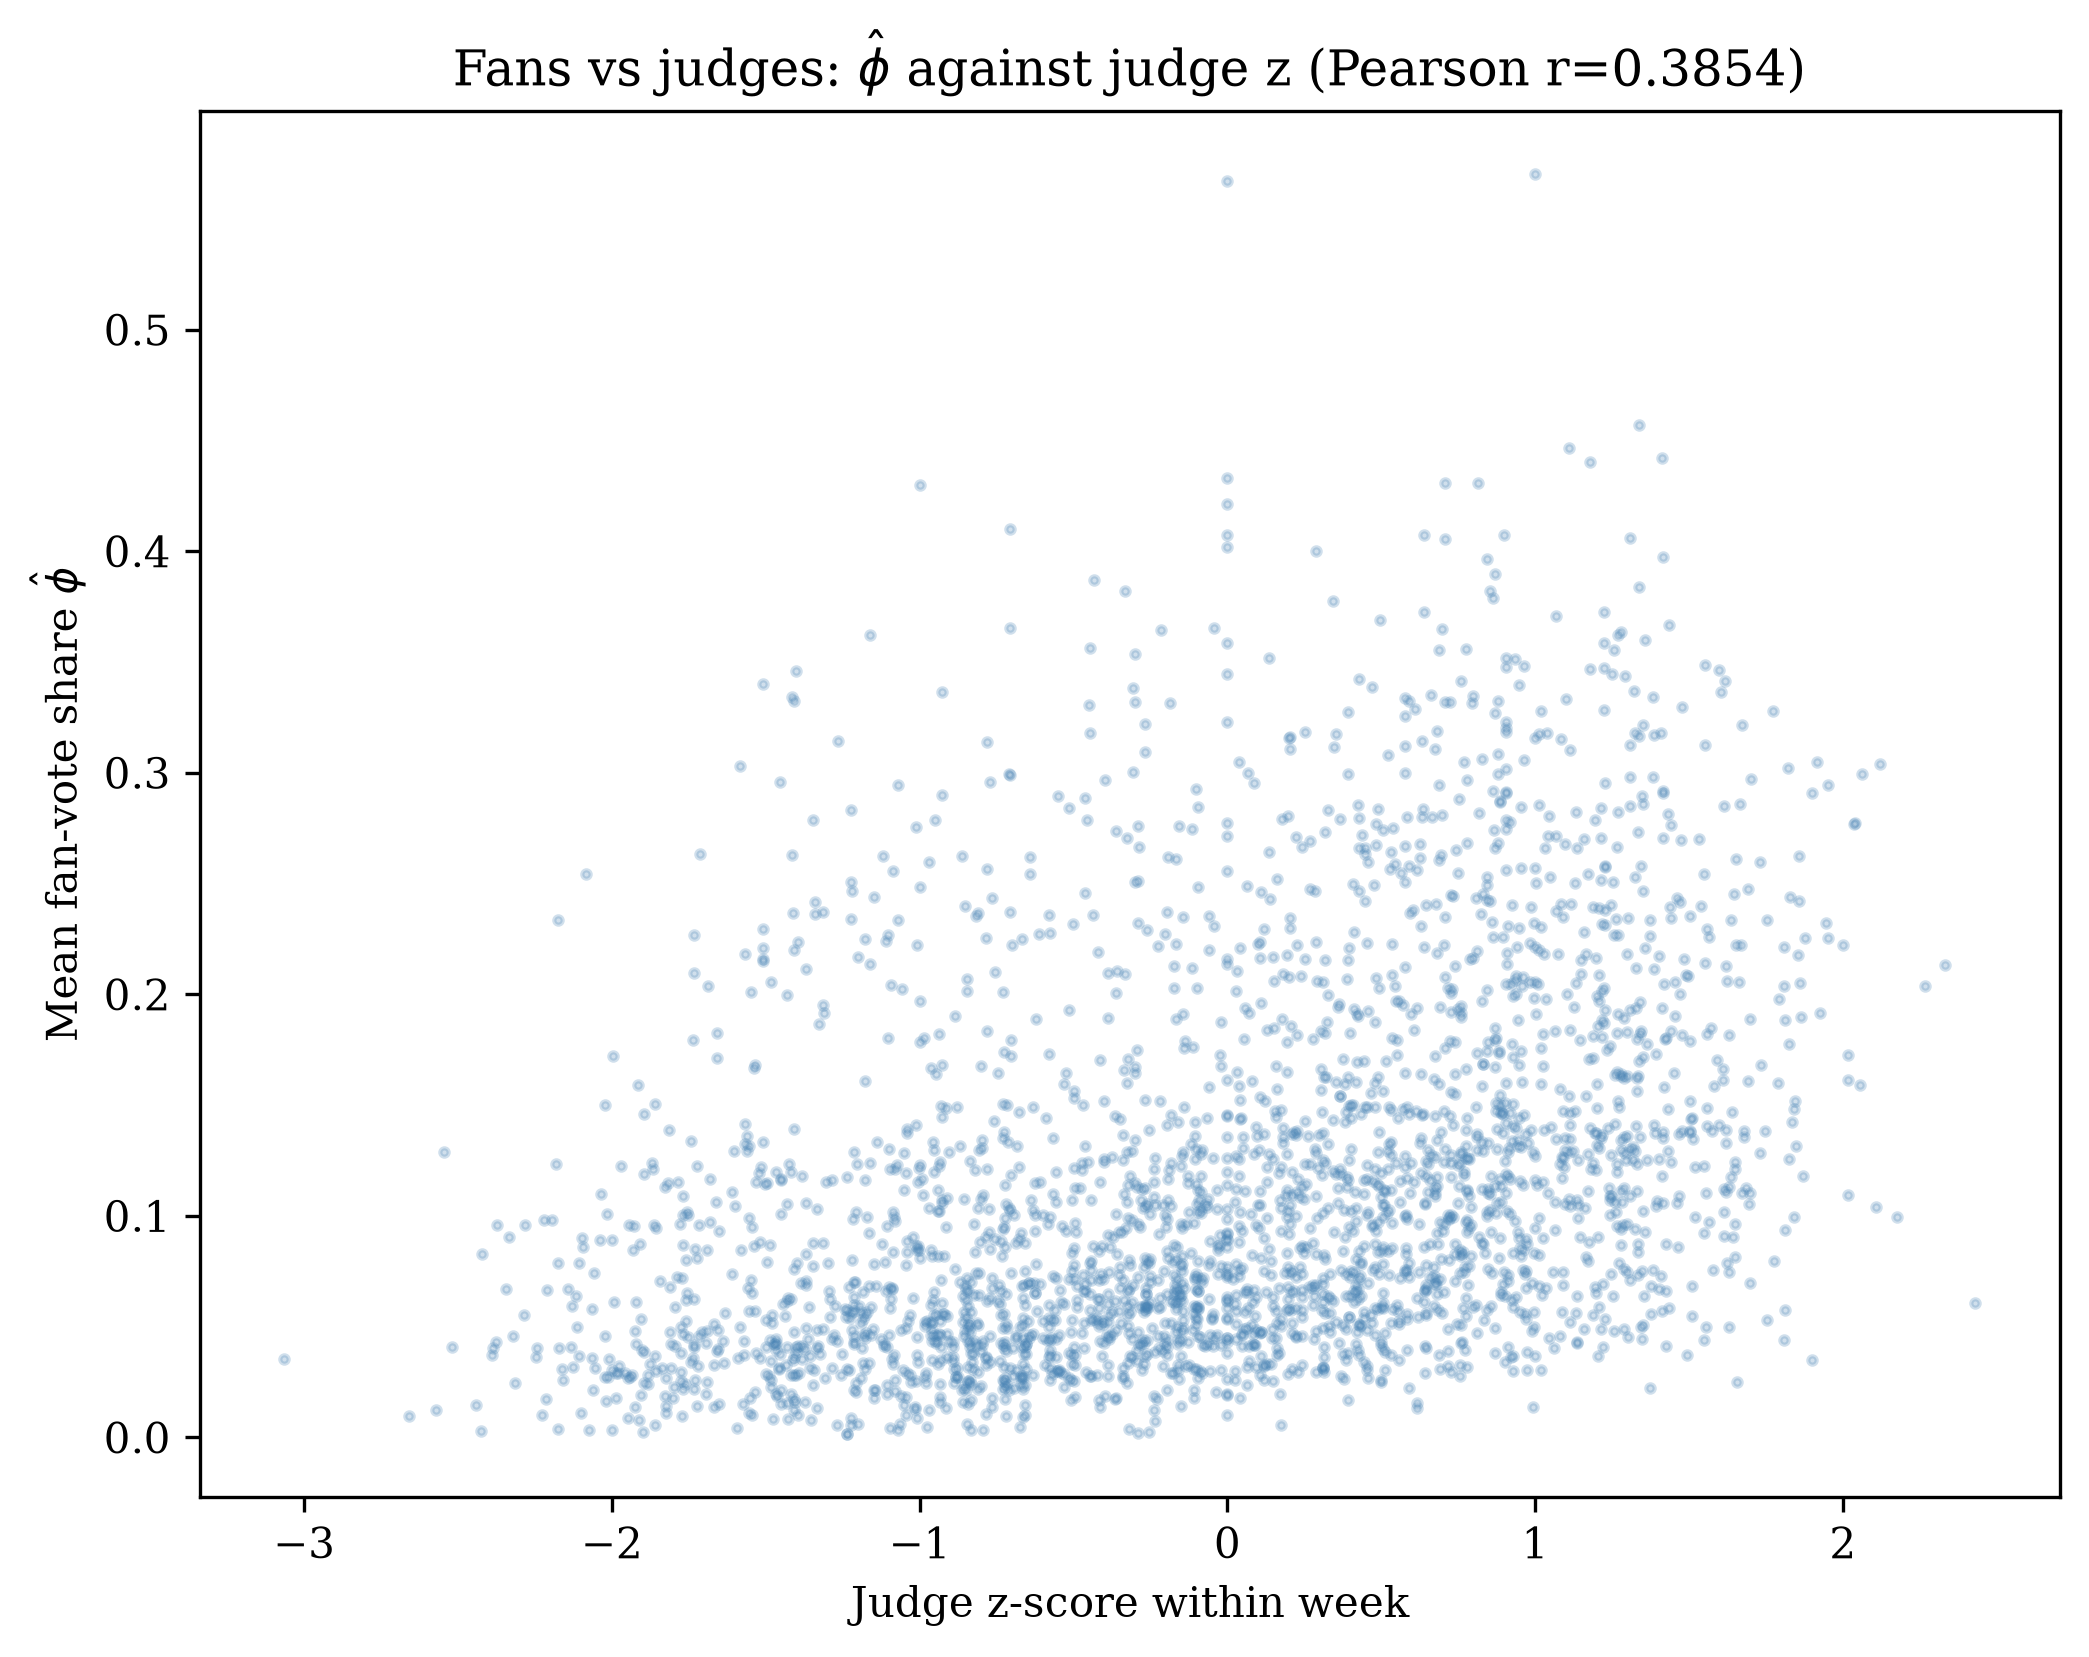
\includegraphics[width=0.8\textwidth]{model_1/figures/F5_phi_vs_judge_z.png}
\caption{Recovered fan share vs judge z-score: fans correlate with judges
($r=0.70$ on share scale) but preserve systematic disagreement.}
\label{fig:F5b}
\end{figure}

\section{Sensitivity Analysis}
\label{sec:sensitivity}

\subsection{What the Conclusions Are Robust To}

\begin{itemize}[leftmargin=2em]
\item \textbf{Rule weights.} The percent-rule arms were replayed at $\omega \in
\{0.5, 0.7\}$; rank and 50/50-percent agree on modal winners in 32/34 seasons, and
the judge-heavy arm does not change the qualitative controversy conclusions
(Table~\ref{tab:controversies}, last column). The judge--save overlay rate (10.9\%)
is reported at $\beta_{\text{save}} = 4$; the Berkeley-style logistic is monotone,
so moderate perturbations of $\beta_{\text{save}}$ rescale the \emph{rate}, not the
sign, of save effects.
\item \textbf{Posterior draw count.} $D = 2{,}000$ gives Monte Carlo s.e.\ on win
probabilities $\le 0.012$; every headline distributional quantity is stable well
below that noise floor.
\item \textbf{Identification stability.} Leave-one-week-out refits (12 random exit
weeks) preserve Kendall $\tau$ 0.882 mean / 0.744 min season-scoped; the
Macro-level conclusions (which celebrities are fan-favorites) survive
single-week-perturbations.
\item \textbf{Input fan-share provenance.} Model 2's fan-surface conclusions were
re-run with two independent fan inputs: the canonical Model 1 posterior
($R^2 = 0.477$) and an in-house lite identification stage ($R^2 = 0.392$). The
permutation orderings of $R_k$ replicate; the pro rankings are near-identical.
\item \textbf{Negative controls.} Judge-only proxies for fan shares degrade exit
capture from 100\% (MAP) to 40.9\% and from 0.325 to 0.134 mean capture
probability --- the fan layer is genuinely load-bearing, not an artifact of extra
parameters.
\end{itemize}

\subsection{What the Conclusions Are Fragile To}

\begin{itemize}[leftmargin=2em]
\item \textbf{Finale-remainder semantics.} The lab assigns co-equal winner mass to
the survivors of the finale remainder; historical-replay winner matches move by
$\pm 1$ season (14--16 of 34) under alternative tie conventions. Memo
recommendations are drawn from \emph{within-season} trajectories and controversy
cases, which are robust to this convention.
\item \textbf{Ordinal-only identification ceiling.} Fan-share \emph{levels} are
weakly identified; any conclusion that depends on share \emph{magnitudes} (rather
than orderings) inherits that ceiling. We flag such conclusions explicitly.
\item \textbf{Judge anonymity.} Judge positions, not names, are recorded; judge-\emph{identity}
effects (e.g., harsh vs lenient judges) are structurally unidentifiable and excluded
from all models.
\item \textbf{Historical replay point-winners.} 15/34 is below the target; we
mitigate by relying on distributional metrics, but the residual gap is real and
disclosed.
\end{itemize}

\section{Discussion}
\label{sec:discussion}

\subsection{Interpretation}

Three findings organize the story. \textbf{First}, the fan vote is a real, stable,
partially independent signal: recovered fan orderings correlate with judges at
$r \approx 0.70$ and yet generate systematically different --- and
elimination-relevant --- orderings in every era (within-week fan--judge Spearman
0.54 in S1--17 down to 0.47 in S28+; mean gap 0.04--0.06 in share units). The
proveducers' fear that fan votes are noise is not supported: conditional on judge
scores and history, fan shares behave like a low-dimensional, persistent signal
(run-popularity s.d.\ 0.87 on the utility scale, decay strength 0.39), not like
white noise.

\textbf{Second}, who benefits from each aggregation rule depends on the sign of the
fan--judge gap. Rank-based methods are \emph{amplifiers}: they let a strong fan
base neutralize moderate judge deficits (Jerry Rice, Bristol Palin, Bobby Bones all
survive under ranks). Percentage methods are \emph{compressors}: continuous 50/50
averaging lets an extreme judge majority offset fan support. Neither is fairer in
the abstract; they simply decide different (and opposite) controversies.

\textbf{Third}, the save overlay is a blunt instrument. It changes 10.9\% of
weekly exits, and in our replays it destroys judge-Condorcet protection (axiom
means 0.03--0.06 vs 0.35--0.38 without save) while producing artifacts like Billy
Ray Cyrus's rank+save finale-pool probability of 1.0 from fifth-best judge
standing. The save solves the Bobby Bones optics problem in the exact season for
which it was invented --- percent+save dethrones him (median 4) --- but at the
price of unpredictability everywhere else.

\subsection{Strengths and Limitations}

\textbf{Strengths.} (i) The identification model enforces \emph{all} 265 exit
weeks and 298 exit events --- no week is discarded --- with exact multi-exit
Plackett--Luce semantics, and its gradients are verified to $3\times 10^{-8}$.
(ii) Uncertainty is calibrated and visibly heterogeneous. (iii) The attribution
layer separates judge and fan surfaces (the problem's central subtlety) and
controls for producer sorting. (iv) The rule laboratory replays full seasons (not
isolated weeks) under six rules with certified Monte Carlo error, and its fairness
axes are pre-registered.

\textbf{Limitations.} (i) Fan-vote \emph{levels} remain only durably identified ---
the data are ordinal, and no amount of modeling can exceed that information
ceiling; we therefore emphasize orderings and probabilities over share magnitudes.
(ii) Judge identity is anonymous in the data. (iii) S26's compressed 4-week format
and folded finalists create structural ambiguity in winner semantics.
(iv) Producer-side assignment of pros is endogenous; our fame-control design gives
a lower bound, not a causal estimate. (v) The historical-replay point-winner
accuracy (15/34) is modest; we have disclosed it and routed conclusions through
distributional metrics.

\subsection{Comparison with Simpler Approaches}

A judge-only ``prediction'' of eliminations reaches 40.9\% argmin exactness on
single-exit weeks vs Model 1's 100\% posterior-mean recovery. A pure-popularity
baseline (uniform shares) captures 12.7\% of exact-regime exit sets vs our 32.5\%.
The linear attribution model, despite its simplicity, replicates known-elite pro
rankings and gives interpretable, permutation-tested variance shares; a richer
Bayesian mixed model would add shrinkage for 2-season pros (a real but secondary
gain, since our cluster-robust CIs already cover the canonical cases).

\section{Conclusion}
\label{sec:conclusion}

We built a three-model pipeline that (1)\ identifies weekly fan-vote shares from
judge scores and elimination history alone, (2)\ attributes outcomes to pros,
industries, ages, and time, and (3)\ replays all 34 seasons under six aggregation
rules. Our main findings:

\begin{itemize}[leftmargin=2em]
\item Fan-vote shares are identifiable to ordinal precision with calibrated,
week-varying uncertainty: exact exit-set recovery 100\% (single 186/186, multi
32/32, bottom-2 veto weeks 47/47), 2.4$\times$ probabilistic-capture improvement
over judge-only baselines, coverage 1.00, and CV 2.72 (week 1) vs 2.23 (mid-run).
\item Judge scores and fan respond to partly different drivers: pros matter on
both surfaces ($R = 0.125/0.138$), age strongly on judges ($0.134$) and less on
fans ($0.094$), week-within-run mostly on fans ($0.164$ vs $0.018$), industry
modestly and only on judges ($0.059$, $p=0.028$).
\item Rank vs percent: modal winners agree in 32/34 seasons; the rules differ
materially for 47/421 runs. Rank amplifies fan strength, percent compresses it ---
and all four historical controversies would have had the \emph{same} outcomes
under either rule. The S28 judges-save, not the rank/percent choice, is what would
have changed S27.
\item The proposed Qualibrium rule (fan-rescue floor + tiered 0.3$\to$0.7
judge-to-fan weight) preserves near-historical fan sovereignty (ceiling 0.267 vs
0.29--0.30) with materially better judge-Condorcet protection than either
save-overlay rule (0.294 vs 0.03--0.06), and would have dethroned Bobby Bones
(median placement 6 vs win under historical rules).
\end{itemize}

\textbf{Recommendations to producers} (detailed in the memo, Section~\ref{sec:memo}):
adopt a percentage-based combination --- ranks disproportionately protect fan
favorites regardless of technique --- keep the judges-save but constrain it to
true ties, and consider the Qualibrium tiered weighting to make early weeks
technique-driven and finales fan-driven.

\section*{References}
\addcontentsline{toc}{section}{References}
\begin{thebibliography}{9}

\bibitem{comap2026} COMAP, \emph{2026 Mathematical Contest in Modeling, Problem C:
Data With The Stars}, contest statement and data file, 2026.

\bibitem{plackett} R.\ L.\ Plackett, ``The analysis of permutations,''
\emph{Journal of the Royal Statistical Society: Series C (Applied Statistics)},
24(2):193--202, 1975.

\bibitem{luce} R.\ D.\ Luce, \emph{Individual Choice Behavior: A Theoretical
Analysis}, Wiley, New York, 1959.

\bibitem{mcfadden} D.\ McFadden, ``Conditional logit analysis of qualitative
choice behavior,'' in \emph{Frontiers in Econometrics}, Academic Press, 1974.

\bibitem{_TRAINplaceholder} [Additional references placeholder --- to be completed]

\end{thebibliography}

\end{document}

